\documentclass{vkr}
\usepackage[english, russian]{babel} % переносы
\usepackage{graphicx} % для вставки картинок
\graphicspath{{images/}} % путь к изображениям
\usepackage[hidelinks]{hyperref}
\usepackage{float} % определяет метод H для рисунка с переносом на следующую страницу, ели не помещается
\usepackage{pdflscape}
\addto{\captionsrussian}{\renewcommand{\refname}{СПИСОК ИСПОЛЬЗОВАННЫХ ИСТОЧНИКОВ}}
\usepackage{xltabular} % для вставки таблиц
\usepackage{makecell}
\renewcommand\theadfont{} % шрифт в /thead
\usepackage{array} % для определения новых типов столбцов таблиц
\newcolumntype{T}{>{\centering\arraybackslash}X} % новый тип столбца T - автоматическая ширина столбца с выравниванием по центру
\newcolumntype{R}{>{\raggedleft\arraybackslash}X} % новый тип столбца R - автоматическая ширина столбца с выравниванием по правому краю
\newcolumntype{C}[1]{>{\centering\let\newline\\\arraybackslash\hspace{0pt}}m{#1}} % новый тип столбца C - фиксированная ширина столбца с выравниванием по центру
\newcolumntype{r}[1]{>{\raggedleft\arraybackslash}p{#1}} % новый тип столбца r - фиксированная ширина столбца с выравниванием по правому краю
\newcommand{\centrow}{\centering\arraybackslash} % командой \centrow можно центрировать одну ячейку (заголовок) в столбце типа X или p, оставив в оcтальных ячейках другой тип выравнивания
\newcommand{\finishhead}{\endhead\hline\endlastfoot}
\newcommand{\continuecaption}[1]{\captionsetup{labelformat=empty} \caption[]{#1}\\ \hline }
\usepackage{etoolbox}
\AtBeginEnvironment{xltabular}{\refstepcounter{tablecnt}} % подсчет таблиц xltabular, обычные таблицы подсчитываются в классе

\usepackage[tableposition=top]{caption} % подпись таблицы вверху
\captionsetup{strut=off}
\setlength{\intextsep}{0pt} % Vertical space above & below [h] floats
\setlength{\textfloatsep}{0pt} % Vertical space below (above) [t] ([b]) floats
\DeclareCaptionLabelFormat{gostfigure}{Рисунок #2} %подпись рисунка
\DeclareCaptionLabelFormat{gosttable}{Таблица #2} %подпись таблицы
\DeclareCaptionLabelSeparator{gost}{~--~} %разделитель в рисунках и таблицах
\captionsetup{labelsep=gost}
\captionsetup[figure]{aboveskip=10pt,belowskip=4mm,justification=centering,labelformat=gostfigure} % настройка подписи рисунка
\captionsetup[table]{font={stretch=1.41},skip=0pt,belowskip=0pt,aboveskip=8.5pt,singlelinecheck=off,labelformat=gosttable} % настройка подписи таблицы

\setlength{\LTpre}{8mm} % отступ сверху таблицы
\setlength{\LTpost}{6mm} % отступ снизу таблицы

\usepackage{enumitem}
\setlist{nolistsep,wide=\parindent,itemindent=*} % отступы вокруг списков, выравнивание с учетом разделителя

\usepackage{color} %% это для отображения цвета в коде
\usepackage{listings} %% листинги кода
\setmonofont[Scale=0.7]{Verdana} % моноширный шрифт для листинга

\definecolor{codegreen}{rgb}{0,0.6,0}
\definecolor{codegray}{rgb}{0.5,0.5,0.5}
\definecolor{codepurple}{rgb}{0.58,0,0.82}

\lstset{ %
	language=C,                 % выбор языка для подсветки (здесь это С)
	numbers=left,               % где поставить нумерацию строк (слева\справа)
	numberstyle=\tiny,           % размер шрифта для номеров строк
	stepnumber=1,                   % размер шага между двумя номерами строк
	numbersep=5pt,                % как далеко отстоят номера строк от подсвечиваемого кода
	commentstyle=\color{codegreen},
	keywordstyle=\color{magenta},
	numberstyle=\tiny\color{codegray},
	stringstyle=\color{codepurple},
	basicstyle=\linespread{0.95}\ttfamily,
	backgroundcolor=\color{white}, % цвет фона подсветки - используем \usepackage{color}
	showspaces=false,            % показывать или нет пробелы специальными отступами
	showstringspaces=false,      % показывать или нет пробелы в строках
	showtabs=false,             % показывать или нет табуляцию в строках
	frame=single,              % рисовать рамку вокруг кода
	tabsize=2,                 % размер табуляции по умолчанию равен 2 пробелам
	captionpos=t,              % позиция заголовка вверху [t] или внизу [b] 
	breaklines=true,           % автоматически переносить строки (да\нет)
	breakatwhitespace=false, % переносить строки только если есть пробел
	escapeinside={\%*}{*)}   % если нужно добавить комментарии в коде
}

\makeatletter % чтобы допускались русские комментарии в листингах
\lst@InputCatcodes
\def\lst@DefEC{%
	\lst@CCECUse \lst@ProcessLetter
	^^80^^81^^82^^83^^84^^85^^86^^87^^88^^89^^8a^^8b^^8c^^8d^^8e^^8f%
	^^90^^91^^92^^93^^94^^95^^96^^97^^98^^99^^9a^^9b^^9c^^9d^^9e^^9f%
	^^a0^^a1^^a2^^a3^^a4^^a5^^a6^^a7^^a8^^a9^^aa^^ab^^ac^^ad^^ae^^af%
	^^b0^^b1^^b2^^b3^^b4^^b5^^b6^^b7^^b8^^b9^^ba^^bb^^bc^^bd^^be^^bf%
	^^c0^^c1^^c2^^c3^^c4^^c5^^c6^^c7^^c8^^c9^^ca^^cb^^cc^^cd^^ce^^cf%
	^^d0^^d1^^d2^^d3^^d4^^d5^^d6^^d7^^d8^^d9^^da^^db^^dc^^dd^^de^^df%
	^^e0^^e1^^e2^^e3^^e4^^e5^^e6^^e7^^e8^^e9^^ea^^eb^^ec^^ed^^ee^^ef%
	^^f0^^f1^^f2^^f3^^f4^^f5^^f6^^f7^^f8^^f9^^fa^^fb^^fc^^fd^^fe^^ff%
	^^^^20ac^^^^0153^^^^0152%
	% Basic Cyrillic alphabet coverage
	^^^^0410^^^^0411^^^^0412^^^^0413^^^^0414^^^^0415^^^^0416^^^^0417%
	^^^^0418^^^^0419^^^^041a^^^^041b^^^^041c^^^^041d^^^^041e^^^^041f%
	^^^^0420^^^^0421^^^^0422^^^^0423^^^^0424^^^^0425^^^^0426^^^^0427%
	^^^^0428^^^^0429^^^^042a^^^^042b^^^^042c^^^^042d^^^^042e^^^^042f%
	^^^^0430^^^^0431^^^^0432^^^^0433^^^^0434^^^^0435^^^^0436^^^^0437%
	^^^^0438^^^^0439^^^^043a^^^^043b^^^^043c^^^^043d^^^^043e^^^^043f%
	^^^^0440^^^^0441^^^^0442^^^^0443^^^^0444^^^^0445^^^^0446^^^^0447%
	^^^^0448^^^^0449^^^^044a^^^^044b^^^^044c^^^^044d^^^^044e^^^^044f%
	^^^^0401^^^^0451%
	%%%
	^^00}
\lst@RestoreCatcodes
\makeatother

% Режим шаблона (должен быть включен один из трех)
\ВКРtrue
%\Практикаtrue
%\Курсоваяtrue

\newcommand{\Дисциплина}{<<Проектирование и архитектура программных систем>>} % для курсовой
\newcommand{\КодСпециальности}{09.03.04} % Курсовая
\newcommand{\Специальность}{Программная инженерия} % Курсовая
\newcommand{\Тема}{} % ВКР Курсовая
\newcommand{\ТемаВтораяСтрока}{Интернет-магазин декоративных растений}
\newcommand{\ГдеПроводитсяПрактика}{ООО «Предприятие ВТИ-Сервис»} % для практики
\newcommand{\РуководительПрактПредпр}{Федосов Д. В.} % для практики
\newcommand{\ДолжнРуководительПрактПредпр}{директор} % для практики
\newcommand{\РуководительПрактУнивер}{Чаплыгин А. А.} % для практики
\newcommand{\ДолжнРуководительПрактУнивер}{к.т.н. доцент} % для практики
\newcommand{\Автор}{И. Р. Головина}
\newcommand{\АвторРод}{Головиной И.Р.}
\newcommand{\АвторПолностьюРод}{Головиной Ирины Романовны} % для практики
\newcommand{\Шифр}{20-06-0175}
\newcommand{\Курс}{4 } % для практики
\newcommand{\Группа}{ПО-02б}
\newcommand{\Руководитель}{Е. И. Аникина} % для ВКР и курсовой
\newcommand{\Нормоконтроль}{А. А. Чаплыгин} % для ВКР
\newcommand{\ЗавКаф}{А. В. Малышев} % для ВКР
\newcommand{\ДатаПриказа}{«04» апреля 2024~г.} % для ВКР
\newcommand{\НомерПриказа}{1616-с} % для ВКР
\newcommand{\СрокПредоставления}{«11» июня 2024~г.} % для ВКР, курсового

\begin{document}
\maketitle
\ifПрактика{}\else{
   \newpage
\begin{center}
\large\textbf{Минобрнауки России}

\large\textbf{Юго-Западный государственный университет}
\vskip 1em
\normalsize{Кафедра программной инженерии}
\vskip 1em
\ifВКР{
        \begin{flushright}
        \begin{tabular}{p{.4\textwidth}}
        \centrow УТВЕРЖДАЮ: \\
        \centrow Заведующий кафедрой \\
        \hrulefill \\
        \setarstrut{\footnotesize}
        \centrow\footnotesize{(подпись, инициалы, фамилия)}\\
        \restorearstrut
        «\underline{\hspace{1cm}}»
        \underline{\hspace{3cm}}
        20\underline{\hspace{1cm}} г.\\
        \end{tabular}
        \end{flushright}
        }\fi
\end{center}
\vspace{1em}
  \begin{center}
  \large
\ifВКР{
ЗАДАНИЕ НА ВЫПУСКНУЮ КВАЛИФИКАЦИОННУЮ РАБОТУ
  ПО ПРОГРАММЕ БАКАЛАВРИАТА}
  \else
ЗАДАНИЕ НА КУРСОВУЮ РАБОТУ (ПРОЕКТ)
\fi
\normalsize
  \end{center}
\vspace{1em}
{\parindent0pt
  Студента \АвторРод, шифр\ \Шифр, группа \Группа
  
1. Тема «\Тема\ \ТемаВтораяСтрока»
\ifВКР{
утверждена приказом ректора ЮЗГУ от \ДатаПриказа\ № \НомерПриказа
}\fi.

2. Срок предоставления работы к защите \СрокПредоставления

3. Исходные данные для создания программной системы:

3.1. Перечень решаемых задач:}

\renewcommand\labelenumi{\theenumi)}

\begin{enumerate}
\item проанализировать IT-инфраструктуру предприятия;
\item  разработать концептуальную модель системы управления IT-ин\-фра\-струк\-турой предприятия на основе подхода к управлению и организации ИТ-услуг ITSM;
\item спроектировать программную систему управления IT-ин\-фра\-струк\-турой предприятия;
\item сконструировать и протестировать программную систему управления IT-инфраструктурой предприятия.
\end{enumerate}

{\parindent0pt
  3.2. Входные данные и требуемые результаты для программы:}

\begin{enumerate}
\item Входными данными для программной системы являются: данные
справочников комплектующих, конфигураций, ПО, критериев качества SLA,
ИТ-услуг, департаментов компании; технические данные ИТ-ресурсов; данные входящих заявок на ИТ-ресурсы; данные запросов поставщикам на комплектующие.
\item Выходными данными для программной системы являются: сформированные заявки на обслуживание ИТ-ресурсов; сформированные запросы на
закупку комплектующих; сведения о выполненных работах по заявкам; статусы заявок; выходные отчеты (инфографика) – по качеству услуг, по состоянию ИТ-ресурсов, по деятельности ИТ-отдела, по стоимости обслуживания
ИТ-ресурсов, воронка заявок.
\end{enumerate}

{\parindent0pt

  4. Содержание работы (по разделам):
  
  4.1. Введение
  
  4.1. Анализ предметной области
  
4.2. Техническое задание: основание для разработки, назначение разработки,
требования к программной системе, требования к оформлению документации.

4.3. Технический проект: общие сведения о программной системе, проект
данных программной системы, проектирование архитектуры программной системы, проектирование пользовательского интерфейса программной системы.

4.4. Рабочий проект: спецификация компонентов и классов программной системы, тестирование программной системы, сборка компонентов программной системы.

4.5. Заключение

4.6. Список использованных источников

5. Перечень графического материала:

\списокПлакатов

\vskip 2em
\begin{tabular}{p{6.8cm}C{3.8cm}C{4.8cm}}
Руководитель \ifВКР{ВКР}\else работы (проекта) \fi & \lhrulefill{\fill} & \fillcenter\Руководитель\\
\setarstrut{\footnotesize}
& \footnotesize{(подпись, дата)} & \footnotesize{(инициалы, фамилия)}\\
\restorearstrut
Задание принял к исполнению & \lhrulefill{\fill} & \fillcenter\Автор\\
\setarstrut{\footnotesize}
& \footnotesize{(подпись, дата)} & \footnotesize{(инициалы, фамилия)}\\
\restorearstrut
\end{tabular}
}

\renewcommand\labelenumi{\theenumi.}

   \abstract{РЕФЕРАТ}

Объем работы равен \formbytotal{lastpage}{страниц}{е}{ам}{ам}. Работа содержит \formbytotal{figurecnt}{иллюстраци}{ю}{и}{й}, \formbytotal{tablecnt}{таблиц}{у}{ы}{}, \arabic{bibcount} библиографических источников и \formbytotal{числоПлакатов}{лист}{}{а}{ов} графического материала. Количество приложений – 2. Графический материал представлен в приложении А. Фрагменты исходного кода представлены в приложении Б.

Перечень ключевых слов: интернет-магазин, растения, база данных, пользователь, администратор, покупатель, товар, web-сайт.

Объектом разработки является интернет-магазин декоративных растений.

Целью выпускной квалификационной работы является создание сайта с основными функциями интернет-магазина и представлением характеристик растений в удобной для пользователя форме.

В процессе создания сайта были выделены основные характеристики растений, на основе которых была построена база данных. Использованы классы и методы модулей, обеспечивающие работу с сущностями предметной области, а также корректную работу интернет-магазина.

При разработке сайта использовался фреймворк Laravel.

Программная система может быть использована для перевода питомника или магазина декоративных растений в онлайн-формат с целью привлечь аудиторию из других городов.

\selectlanguage{english}
\abstract{ABSTRACT}
  
The volume of work is \formbytotal{lastpage}{page}{}{s}{s}. The work contains \formbytotal{figurecnt}{illustration}{}{s}{s}, \formbytotal{tablecnt}{table}{}{s}{s}, \arabic{bibcount} bibliographic sources and \formbytotal{числоПлакатов}{sheet}{}{s}{s} of graphic material. The number of applications is 2. The graphic material is presented in annex A. The layout of the site, including the connection of components, is presented in annex B.

List of keywords: online shop, plants, database, user, administrator, buyer, goods, web site.

The object of the development is an online shop of decorative plants.

The purpose of the final qualification work is to create a website with the main functions of an online shop and the presentation of plant characteristics in a user-friendly form.

In the process of creating the site, the main characteristics of plants were highlighted, on the basis of which the database was built. Classes and methods of modules were used to ensure work with the entities of the subject area, as well as the correct operation of the online shop.

The Laravel framework was used in the development of the site.

The software system can be used to convert a nursery or an decorative plant store into an online format in order to attract an audience from other cities.
\selectlanguage{russian}
}\fi
\tableofcontents
\section*{ОБОЗНАЧЕНИЯ И СОКРАЩЕНИЯ}

БД -- база данных.

ИС -- информационная система.

ИТ -- информационные технологии. 

%КТС -- комплекс технических средств.

%ОМТС -- отдел материально-технического снабжения. 

ПО -- программное обеспечение.

РП -- рабочий проект.

СУБД -- система управления базами данных.

ТЗ -- техническое задание.

ТП -- технический проект.

UML (Unified Modelling Language) -- язык графического описания для объектного моделирования в области разработки программного обеспечения.

\ifПрактика{}\else{\section*{ВВЕДЕНИЕ}
\addcontentsline{toc}{section}{ВВЕДЕНИЕ}

Питомник растений – это специально созданный участок, где выращивают и продают различные виды и сорта растений. Они могут быть как крупными промышленными предприятиями, так и небольшими семейными бизнесами. Главная задача питомников — производить качественные растения с хорошо развитой корневой системой, которые могут быстро адаптироваться к новым условиям роста. Растения в питомниках продаются как оптом, так и в розницу.

Из-за больших размеров и требований к окружающей среде, питомники не всегда удобно располагать в местах с большим скоплением людей. Однако они должны быть расположены вблизи населённых пунктов, чтобы обеспечить удобный доступ для покупателей и крупной техники.

Интернет-магазин позволяет привлекать покупателей из разных городов и требует гораздо меньше средств, чем открытие филиалов и привлечение дистрибьюторов. Кроме того, покупка через Интернет занимает у покупателя меньше времени, что увеличивает вероятность её совершения. Также есть возможность принимать заказы по ночам, когда физические магазины обычно не работают.

Ещё одним преимуществом создания интернет-магазина является возможность использовать маркетинговые инструменты для продвижения. Благодаря сайту можно реализовать таргетированную рекламу, поисковую оптимизацию (SEO), аналитику и многое другое.

Сайт является лицом компании и может существенно повысить её имидж. Любой пользователь Интернета сможет получить необходимую информацию о компании в любое время. На сайте можно найти контактные телефоны, адрес и электронную почту для связи с компанией. Сейчас большинство клиентов узнают о её существовании именно через сайт. Поэтому сайт можно назвать лучшей рекламой.

\emph{Цель настоящей работы} – разработка web-сайта для продажи растений через Интернет. Для достижения поставленной цели необходимо решить \emph{следующие задачи:}
\begin{itemize}
	\item провести анализ предметной области;
	\item разработать концептуальную модель web-сайта;
	\item спроектировать web-сайт;
	\item реализовать сайт средствами web-технологий.
\end{itemize}

\emph{Структура и объем работы.} Отчет состоит из введения, 4 разделов основной части, заключения, списка использованных источников, 2 приложений. Текст выпускной квалификационной работы равен \formbytotal{page}{страниц}{е}{ам}{ам}.

\emph{Во введении} сформулирована цель работы, поставлены задачи разработки, описана структура работы, приведено краткое содержание каждого из разделов.

\emph{В первом разделе} на стадии описания технической характеристики предметной области приводится сбор информации о характеристиках растений и специфике продажи товаров через Интернет.

\emph{Во втором разделе} на стадии технического задания приводятся требования к разрабатываемому сайту.

\emph{В третьем разделе} на стадии технического проектирования представлены проектные решения для web-сайта.

\emph{В четвертом разделе} приводится спецификация контроллеров приложения, производится тестирование разработанного сайта.

В заключении излагаются основные результаты работы, полученные в ходе разработки.

В приложении А представлен графический материал.
В приложении Б представлены фрагменты исходного кода.

}\fi
\section{Анализ предметной области}
\subsection{Особенности интернет-торговли растениями}

Продажа семян и саженцев по почте — это удобный и популярный способ покупки в России. Больше не нужно обходить множество магазинов в поисках нужных сортов и гибридов: покупатели могут спокойно и внимательно изучить каталог или сайт интернет-магазина, не выходя из дома.

Во многих регионах страны выбор семян и посадочного материала ограничен, а качество и ассортимент уступают тем, что представлены в крупных интернет-магазинах и каталогах компаний. Поэтому жители регионов часто заказывают товары по почте, так как не могут найти нужный сорт или вид растения в обычных магазинах.

Дистанционная торговля семенами и посадочным материалом может осуществляться двумя способами: через каталоги и через интернет-магазины. До недавнего времени основным видом торговли была продажа через каталоги. С развитием интернета в нашей стране, на смену этому виду торговли пришла торговля через интернет-магазины.

Самый популярный и простой товар с точки зрения хранения и доставки — это семена \cite{krivko}. Их можно заказывать круглый год, многие огородники планируют свои посевы ещё с осени и делают заказы заранее, в октябре-декабре. Такие посылки приходят адресату до Нового года. Однако пик заказов обычно приходится на январь-февраль. Заказывая семена, всегда нужно учитывать сроки посева каждой культуры. Затем отнимается 3-5 дней на комплектацию заказа и 5-20 дней на доставку почтой, в зависимости от региона. В итоге получается, что заказ семян следует делать минимум за месяц до посева \cite{kaygorodtseva}.

Второй по популярности товар — это луковичные и многолетние растения. Этот вид товара имеет два сезона продаж — весна и осень. Весной предлагается огромный ассортимент многолетних растений, таких как астильбы, хосты, пионы травянистые, гейхеры, а также луковичных растений, таких как гладиолусы, лилии, амариллисы. Срок приёмки заказов с ноября по апрель, отправка заказов начинается в марте. Осенний сезон более короткий и предлагает тюльпаны, нарциссы, крокусы, гиацинты и различные мелколуковичные растения. Заказы принимаются с июля по август, отправка осуществляется с августа по сентябрь.

Саженцы плодовых и декоративных кустарников и деревьев — следующий по популярности товар. Приём заказов начинается с ноября, а рассылка стартует после 8 марта.

Саженцы кустарников и деревьев, а также луковичные и многолетние растения — это более специфический продукт, чем семена. Для сохранения качества им нужны определённые температурные условия.
При выборе оплаты наложенным платежом покупатель оплачивает посылку при получении на почте. Стоимость посылки состоит из нескольких компонентов: стоимости товара, стоимости доставки, которая зависит от веса посылки, расстояния и выбранного способа доставки, а также комиссии за обработку наложенного платежа, которую взимает почтовая служба или курьерская компания.

При выборе предоплаты покупатель заполняет квитанцию в каталоге или получает её на электронную почту. Отправка заказа осуществляется после поступления денег на расчётный счёт продавца. При получении товара на почте покупатель оплачивает только расходы за почтовую пересылку.


\subsection{Характеристики растений}
Декоративные растения — это разнообразная группа растений, включающая как культивируемые, так и дикие виды деревьев, кустарников, многолетних и однолетних растений, злаков и луковичных растений, которые принадлежат к различным ботаническим семействам. Их уникальные декоративные качества делают их незаменимыми для озеленения садов, парков и скверов, а также для украшения зданий и внутренних помещений.

Внешний облик декоративных растений играет ключевую роль в определении их декоративных характеристик. Важными аспектами являются живописность кроны, изящество силуэта, длительность и обильность цветения, изменчивая окраска в течение года, способность выдерживать неблагоприятные условия и климатические изменения.

Декоративные злаки — это растения семейства злаковых, которые используются для создания групповых посадок и бордюров, газонов, а также для составления букетов. Они обладают привлекательной текстурой и формой, что делает их популярными элементами ландшафтного дизайна \cite{kingsberry}.

Луковичные растения представляют собой обширную группу декоративных растений, различающихся по цвету, размеру, форме цветков и времени цветения. В открытом грунте они цветут с весны до осени, а благодаря зимней выгонке способны цвести практически круглый год. Эти растения могут использоваться для выращивания в помещении и для создания букетов.

С точки зрения распространения по миру, луковичные растения представляют одну из самых многочисленных групп. Они включают в себя преимущественно лилейные и амариллисовые семейства \cite{belyaevskaya}.

Луковичные растения могут размножаться как вегетативным способом, так и семенами. Лилии и гиппеаструмы обычно размножаются семенами, этот метод также используется при создании новых сортов.

Растения, образующие луковицы, требуют особой почвы. Им подходят легкие, проницаемые и влагоемкие грунты с нейтральной или слабощелочной реакцией (pH не ниже 6–7). Последнее особенно важно для тюльпанов. Для лилий подходят легкие глинистые почвы с хорошей дренажной системой, практически без извести. Гиацинты и тюльпаны предпочитают песчаные почвы, богатые питательными веществами, с нейтральной кислотностью. Тяжелые глинистые почвы с плохой водопроницаемостью, а также очень бедные песчаные почвы не подходят для луковичных растений \cite{doroshenko}.

Декоративные деревья и кустарники бывают хвойные и лиственные, вечнозелёные или с опадающей листвой. Их красота зависит от внешних характеристик, таких как форма кроны, цвет и структура листьев, а также цвет и размер цветов и плодов. Подходящие условия для роста помогают сохранить красоту растений, которая меняется вместе с возрастом и сменой времен года в зависимости от генетических особенностей вида.

У древесных растений существуют два способа размножения: семенной и вегетативный. Семенное размножение осуществляется через семена, а вегетативное — через черенки, отводки, корневые отпрыски, прививки или деление куста \cite{berd}.

При создании групп и игры с контрастными цветами важную роль играет окраска листьев деревьев. Она может усилить общее впечатление от кроны, добавить плотности и объема. В течение сезона меняется интенсивность окраски листьев. Форма и размер листьев также влияют на декоративность растений, особенно если они находятся рядом с дорожками. Растения с красивыми и необычными листьями имеют большую ценность в ландшафтном дизайне, если они не характерны для местной флоры.

В период цветения декоративные растения приобретают особую привлекательность. Они отличаются разнообразием форм, цветов, размеров соцветий, ароматами, продолжительностью и временем цветения. Правильный выбор цветущих растений поможет создать композицию с длительным цветением.

Жизненный цикл декоративных растений — это онтогенез, или индивидуальное развитие растения от его появления из оплодотворенной яйцеклетки или вегетативной почки (черенка с почками, корневого отпрыска и т.п.) до отмирания.

\subsubsection{Многолетние растения}

Характерной чертой многолетних травянистых растений является способность переживать зиму на открытой земле, ежегодно проходить через все стадии развития (рост, цветение, плодоношение) и продолжать этот цикл на протяжении многих лет благодаря специальным органам, предназначенным для зимовки (корень, корневище, луковица, ползучие стебли и другие).

У большинства декоративных многолетников надземная часть каждый год отмирает, но на следующий сезон восстанавливается за счет измененного подземного стебля в виде корневищ, луковиц, клубнелуковиц (например, луковичные растения, пионы, флоксы, рудбекия, акониты и другие) \cite{viyginaOpen}.

У других растений надземные побеги не отмирают, а сохраняются зимой, когда все жизненные процессы, как у древесных растений, замедляются. С приходом весны и благоприятных условий из почек начинают развиваться новые вегетативные и генеративные побеги, которые цветут и образуют семена.

У некоторых видов растений стебель и корень, помимо своих основных функций, также выполняют задачи вегетативного размножения и защиты растений зимой.

Существуют три основных типа подземных стеблей: луковица, клубень (клубнелуковица) и корневище.

Луковица – это видоизменённый побег с плотным коротким стеблем и мясистыми листьями, имеющими вид чешуек и запасающими воду и питательные вещества \cite{belyaevskaya}.

Клубень -- это укороченный, значительно утолщенный подземный побег, который запасает питательные вещества. Клубни, имеющие форму луковицы, называются клубнелуковицами.

Корневище -- это долговечное стеблевое образование, внешне напоминающее корень, но отличающееся наличием дополнительных корней и почек. На его поверхности можно видеть следы прикрепления листьев в виде коричневых чешуек и остатки умерших побегов. Корневище может быть горизонтальным, утолщенным (как у ириса, бадана, ландыша), растущим вертикально или наклонно вниз (как у астильбы, примулы, функии, диклитры) \cite{aldohina}.

У многолетних стержнекорневых растений основной корень не замещается дополнительными, а сохраняется на протяжении всей жизни растения. На его поверхности могут быть небольшие корешки с дополнительными почками (корневые отпрыски), используемые для размножения.

Многолетние растения, благодаря своим биологическим особенностям, способны выдерживать низкие температуры зимой. Молодые экземпляры имеют невысокую степень морозоустойчивости, но по мере их развития эта способность увеличивается. Однако по мере завершения жизненного цикла у растений морозоустойчивость снова снижается. Для сохранения и развития этого ценного биологического свойства растений важна своевременная подготовка к зиме, проведение осенних и ранневесенних посевов в открытый грунт. Не столько низкие температуры, сколько резкие перепады могут нанести вред многолетникам. Особенно опасны для них зимы без снега, с оттепелями и долгими затоплениями поверхности почвы водой. Поэтому для выращивания многолетников, особенно тех, что длительное время находятся на одном месте (например, пионы, флоксы, функии и другие), необходимо выбирать ровные, хорошо дренированные участки без застоя воды.

При создании декоративных миксбордеров (цветников-бордюров из смешанных растений разных размеров и оттенков) важно учитывать морозоустойчивость растений и подбирать ассортимент с учетом конкретных почвенно-климатических условий каждой зоны. Только таким образом можно обеспечить успешное процветание и красоту растений в течение долгого времени \cite{karpisonova}.

\subsubsection{Двулетние растения}

В цветоводстве под двулетниками понимаются растения, которые по своей природе являются многолетниками, но достигают пика декоративного эффекта в период своего второго года жизни. К их числу относятся такие виды, как виола, колокольчики, наперстянка, маргаритки и незабудки.

Двулетники обладают разнообразными биологическими и декоративными характеристиками, благодаря чему их применяют для украшения садов и цветников в начале весны, в качестве материала для создания цветочных композиций, для выращивания в горшках, а также для украшения помещений и пристенного озеленения \cite{aldohinaFlower}.

В отличие от однолетников, двулетники не завершают свой жизненный цикл за один сезон. В первый год они формируют мощную розетку листьев, в то время как во втором году достигают максимального цветущего состояния и дают плоды. В ходе третьего зимнего сезона большая часть растений гибнет, но из семян, оставшихся после увядания, вновь появляются новые растения, которые также достигают пика цветения во втором году своей жизни. Таким образом, участки, занятые двулетниками, способны к самовозобновлению и могут сохранять свою декоративность на протяжении многих лет, со временем изменяя свой облик.

При сильной засухе двулетники могут зацвести и дать небольшое количество семян в первый год жизни.

\subsubsection{Однолетние растения}

К группе однолетников относятся однолетние цветочные культуры, которые проходят все стадии развития за один сезон. Это астры, ноготки, бархатцы, васильки, алиссумы, маки, флоксы летние и другие растения.

В год посева они цветут, дают семена и погибают. Продолжительность их жизни — всего несколько месяцев в году. Однако по разнообразию форм, яркости окраски цветков и длительности цветения многие летники превосходят другие цветочные растения. Они обладают исключительным многообразием по всем декоративным особенностям и предоставляют продолжительное время  для срезки в букеты — от апреля до самых морозов. Кроме того, летники имеют ещё одно положительное свойство — их можно пересаживать в цветущем состоянии.

К однолетникам причисляют некоторые грунтовые многолетники, которые зацветают в первый же год, но не переносят зиму в наших условиях. К ним относятся львиный зев, петуния, вербена и другие растения, которые на своей родине живут по несколько лет.

По декоративным качествам и применению в озеленении летники можно разделить на цветущие и лиственно-декоративные (орнаментальные), бордюрные и вьющиеся.

Большой видовой и сортовой ассортимент однолетних растений позволяет выбрать множество однолетников, которые можно размножать безрассадным способом — посевом семян в открытый грунт. Этот способ отличается доступностью и дешевизной.

Посев семян летников можно производить осенью — после окончания периода длительных потеплений (вторая половина ноября — начало декабря), весной — до наступления вегетационного периода (вторая половина апреля) или летом. Весенний посев в большинстве случаев даёт лучшие результаты, чем осенний, поэтому надежнее сеять летники весной.

Непосредственно в открытый грунт весной и осенью высевают семена многих однолетних растений, которые достаточно холодостойки. Более теплолюбивые виды следует высевать только после того, как прекратятся сильные весенние заморозки по утрам.

Также в открытый грунт высевают семена тех растений, которые не переносят пересадку (пикировку) из-за того, что их корневая система не может быстро восстановить всасывающие волоски, которые развиваются только на глубоко уходящих в почву корневых ответвлениях (мак, левкой, резеда, люпин, настурция, эшшольция).

В открытый грунт также высевают семена быстрорастущих видов растений, таких как декоративная фасоль, ноготки, акроклинум, кореопсис и бархатцы.

Для посева однолетних декоративных растений лучше всего использовать крупные отборные семена. Отбор крупных семян имеет огромное преимущество — они содержат большой запас питательных веществ, сеянцы быстро развиваются и образуют сильнорослые устойчивые растения с крупными соцветиями и цветками, которые лучше сопротивляются грибковым заболеваниям и вредителям. Кроме того, в таких случаях наблюдается более раннее цветение \cite{aleksandrova}.


\subsection{Анализ существующих интернет-магазинов}
\label{shopsAnalize}
Анализ существующих сайтов с похожей тематикой позволяет выделять достоинства и недостатки, чтобы использовать эту информацию для улучшения качества собственной разработки.

Существует большое количество интернет-магазинов декоративных растений. Для анализа были выбраны 3 сайта, занимающие верхние строчки в поисковике <<Яндекс>> при запросе <<Интернет-магазин декоративных растений>>:
\begin{itemize}
	\item <<garshinka>>;
	\item <<pervocvet-shop>>;
	\item <<plantmania>>.
\end{itemize}

Все вышеперечисленные сайты имеют такие базовые страницы, как каталог товаров, корзина покупателя и вход в личный кабинет. Наибольший интерес для анализа вызывает каталог товаров, так как  его структура на разных сайтах отличается.

На рисунке ~\ref{garshinka:image} представлен каталог товаров интернет-магазина <<garshinka>>.

\begin{figure}[h!]
	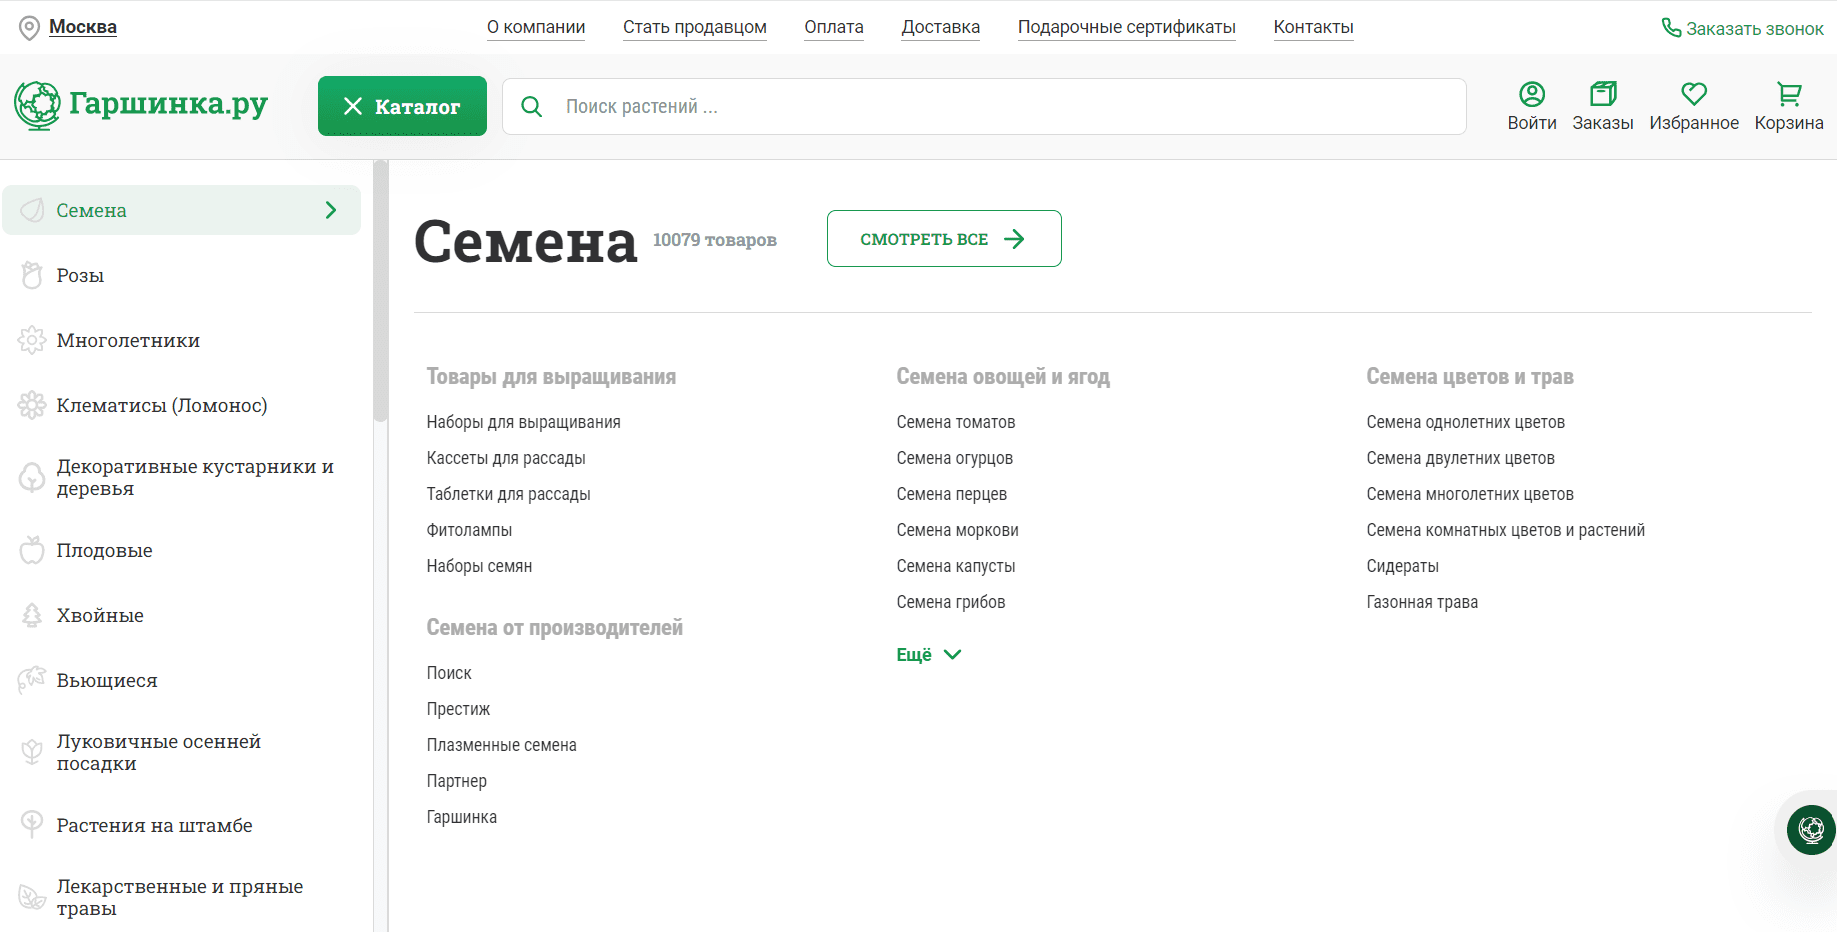
\includegraphics[width=0.8\linewidth]{garshinka}
	\caption{Каталог товаров магазина <<garshinka>>}
	\label{garshinka:image}
\end{figure}
%\vspace{-\figureaboveskip} % двойной отступ не нужен (можно использовать, если раздел заканчивается картинкой)


На рисунке ~\ref{pervocvet:image} представлен каталог товаров интернет-магазина <<pervocvet-shop>>.

\begin{figure}[h!]
	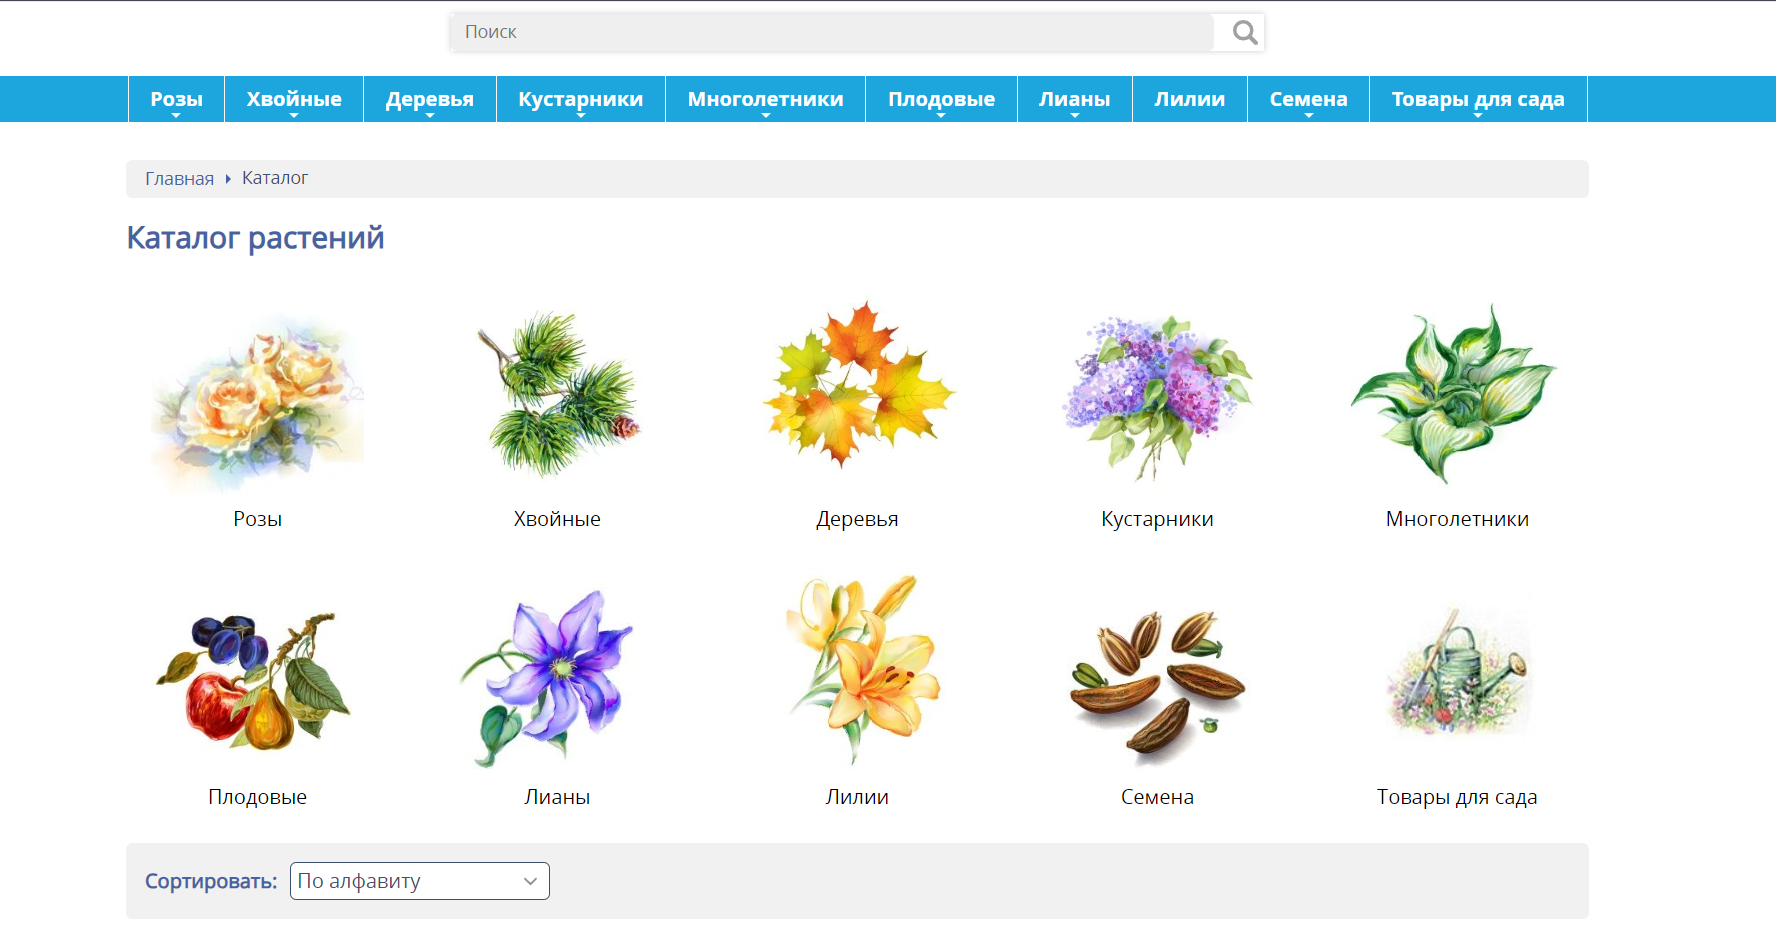
\includegraphics[width=0.8\linewidth]{pervocvet }
	\caption{Каталог товаров магазина <<pervocvet-shop>>}
	\label{pervocvet:image}
\end{figure}
%\vspace{-\figureaboveskip} % двойной отступ не нужен (можно использовать, если раздел заканчивается картинкой)


На рисунке ~\ref{plantmania:image} представлен каталог товаров интернет-магазина <<plantmania>>.

\begin{figure}[h!]
	
\includegraphics[width=0.8\linewidth]{plantmania}
	\caption{Каталог товаров магазина <<plantmania>>}
	\label{plantmania:image}
\end{figure}
%\vspace{-\figureaboveskip} % двойной отступ не нужен (можно использовать, если раздел заканчивается картинкой)


Каждый рассматриваемый магазин имеет категории, упрощающие поиск нужного товара. Можно заметить, что список категорий индивидуален для каждого сайта. Однако имеется общая черта: в список категорий входят разнообразные характеристики растений: жизненный цикл, тип посадочного материала и т.д. Причём, предлагаются не все варианты каждой характеристики: например, на каждом сайте имеется категория <<многолетние растения>>, но не представлены категории для двулетних и однолетних растений. Это позволяет пользователю без труда находить самые популярные категории,  но делает невозможным поиск для пользователя с более редкими требованиями.

Кроме того, все сайты имеют строку для поиска товара по названию, что является однозначным достоинством.


\section{Техническое задание}
\subsection{Основание для разработки}

Полное наименование системы: "<Интернет-магазин декоративных растений">.

Основанием для разработки программы является приказ ректора ЮЗГУ от <<04>> апреля 2024 г. №1616-с <<Об утверждении тем выпускных квалификационных работ>>.


\subsection{Цель и назначение разработки}

Программно-информационная система предназначена для продажи растений через Интернет.
С системой должны работать следующие группы пользователей:
\begin{itemize}
	\item администратор интернет-магазина;
	\item посетитель интернет-магазина.
\end{itemize}

Администратор должен иметь возможность добавлять, удалять и редактировать товары и свои категории. Например, "<акции"> или "<новинки">.
Посетитель интернет-магазина должен иметь возможность просматривать товары, добавлять их в корзину и оформлять заказ.

Задачами данной разработки являются:
\begin{itemize}
	\item проектирование базы данных;
	\item проектирование пользовательского интерфейса;
	\item разработка методов отображения данных из базы данных;
	\item разработка методов управления базой данных администратором.
\end{itemize}

\subsection{Требования к программной системе}

\subsubsection{Требования к данным}
Входными данными для системы являются:
\begin{itemize}
	\item информация о пользователе, предоставляемая им в процессе регистрации в системе;
	\item информация о пользователе, предоставляемая им в процессе оформления заказа;
	\item информация о товарных позициях (отдельных товарах) заказа;
	\item параметры фильтрации товаров;
	\item информация о товарах, вводимая администратором;
	\item информация о категориях, вводимая администратором.
\end{itemize}

Выходными данными для системы являются:
\begin{itemize}
	\item стоимость всех товаров в корзине;
	\item список заказов;
	\item уведомление о добавлении товара в корзину;
	\item уведомление об удалении товара из корзины;
	\item уведомление об оформленном заказе;
	\item сообщения об ошибках;
	\item ссылки для переадресации (URL).
\end{itemize}


\subsubsection{Функциональные требования}

Сайт имеет две группы пользователей с разными правами: администраторы и покупатели.

Администраторам сайта должны быть доступны следующие функции:
\begin{itemize}
	\item просмотр информации о товаре;
	\item редактирование информации о товаре;
	\item удаление товара;
	\item добавление товара;
	\item просмотр информации о заказе;
	\item просмотр информации о категории;
	\item редактирование информации о категории;
	\item удаление категории;
	\item добавление категории.
\end{itemize}

На рисунке ~\ref{admin:image} изображены прецеденты для администратора сайта.

\begin{figure}[h!]
	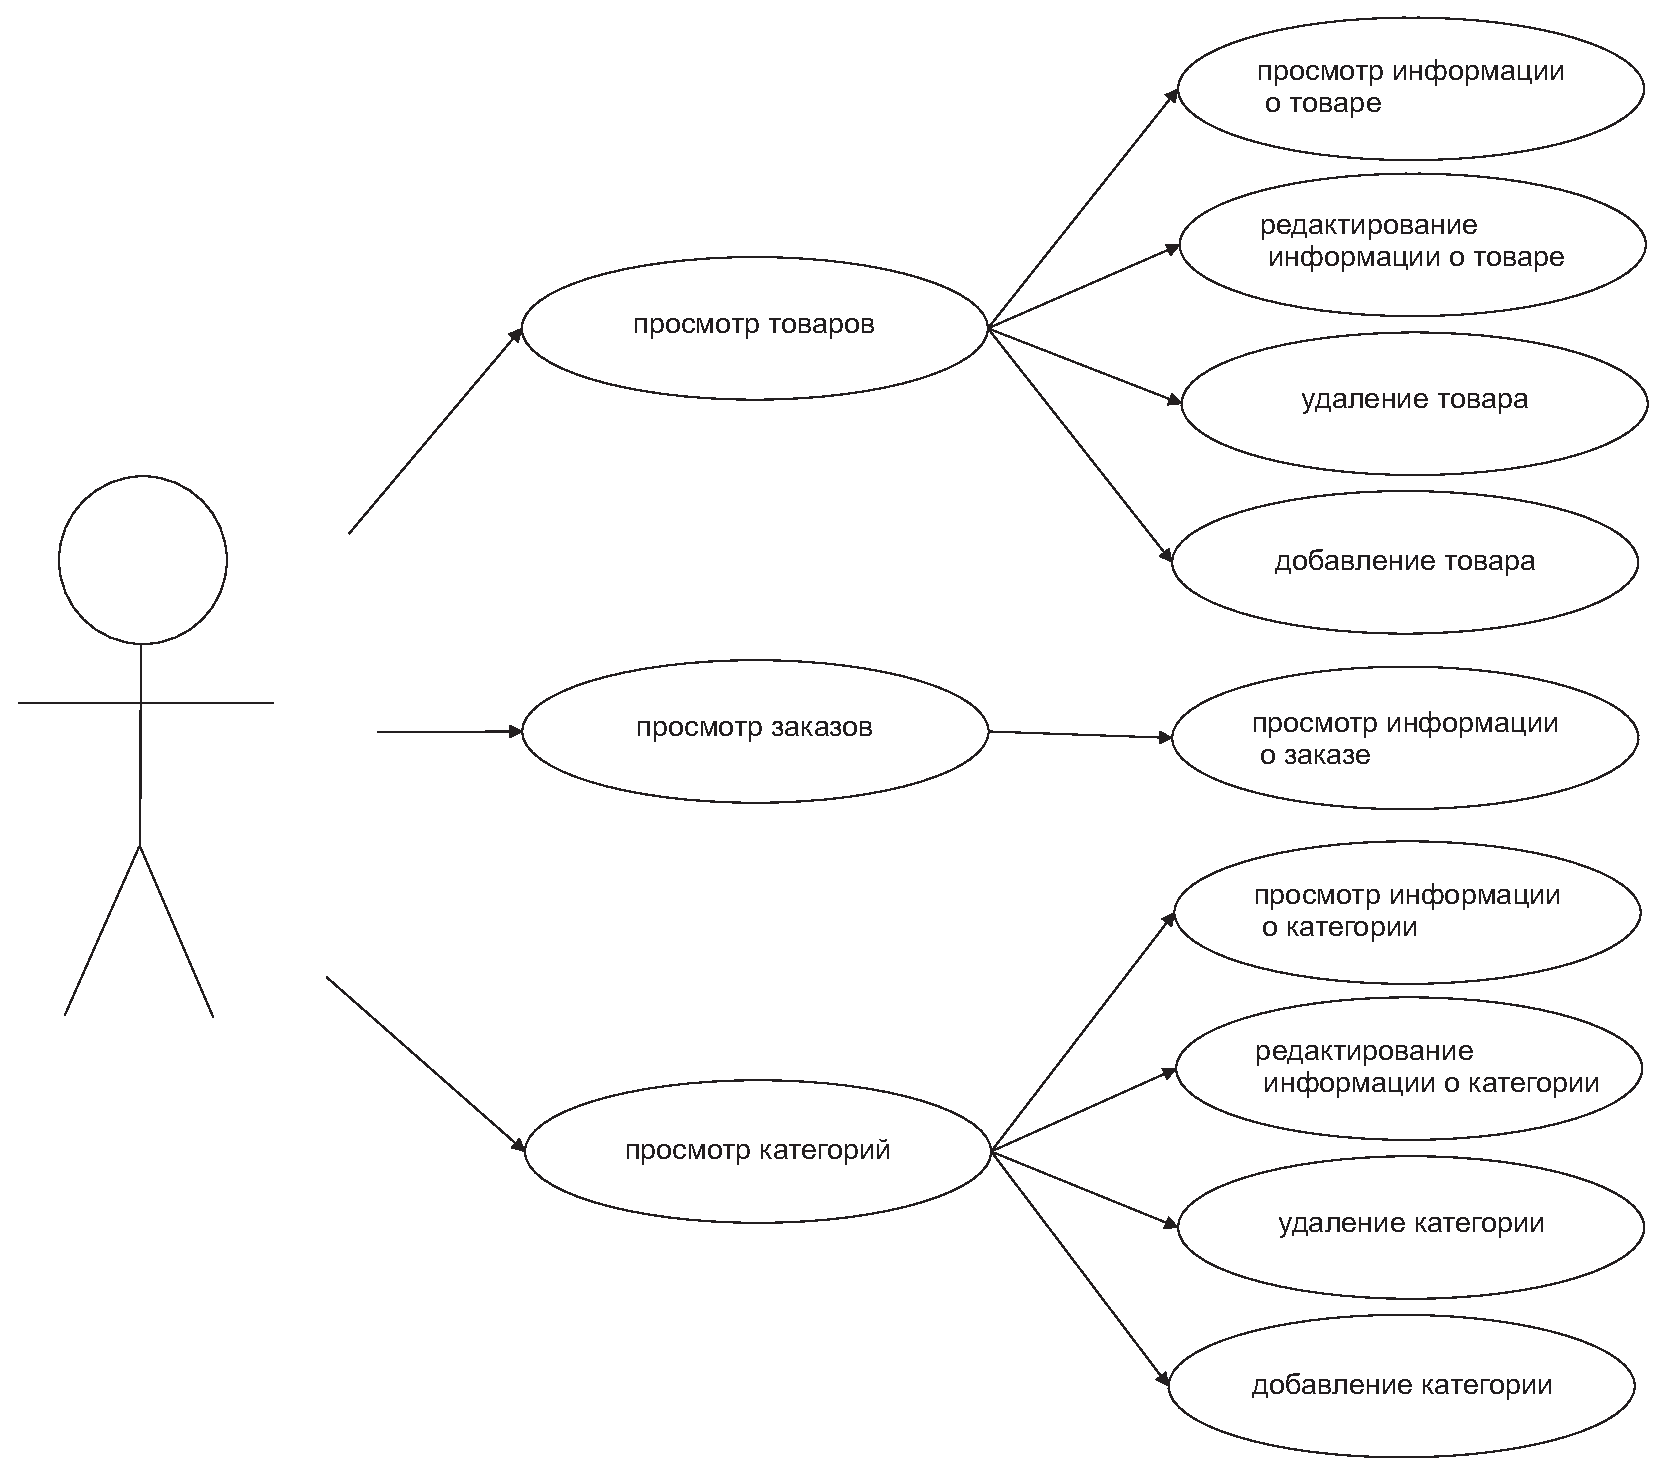
\includegraphics[width=0.8\linewidth]{admin}
	\caption{Прецеденты для администратора}
	\label{admin:image}
\end{figure}
%\vspace{-\figureaboveskip} % двойной отступ не нужен (можно использовать, если раздел заканчивается картинкой)

Покупателям должны быть доступны следующие функции:
\begin{itemize}
	\item просмотр информации о товаре;
	\item добавление товара в корзину;
	\item просмотр товаров категории;
	\item просмотр информации о заказе;
	\item изменение количества товаров в корзине;
	\item оформление заказа.
\end{itemize}

На рисунке ~\ref{user:image} изображены прецеденты для покупателя.
\begin{figure}[h!]
	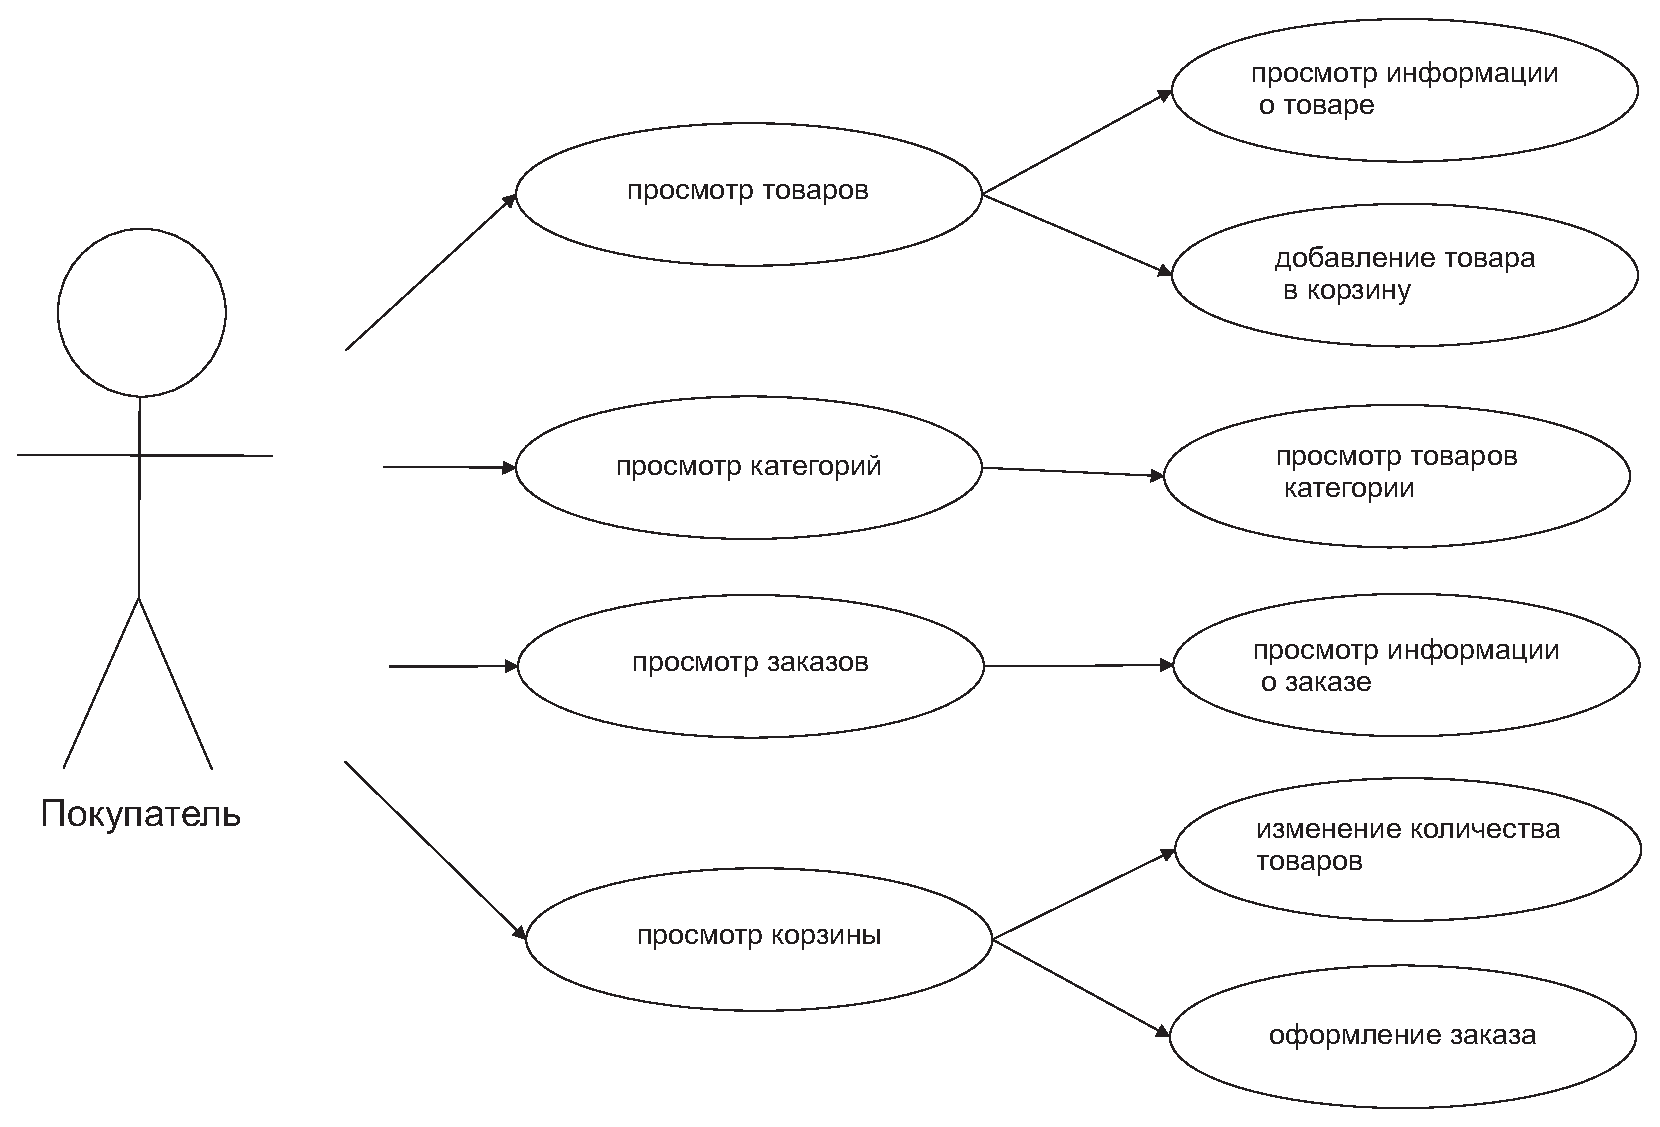
\includegraphics[width=0.8\linewidth]{user}
	\caption{Прецеденты для покупателя}
	\label{user:image}
\end{figure}
%\vspace{-\figureaboveskip} % двойной отступ не нужен (можно использовать, если раздел заканчивается картинкой)


\paragraph{Сценарий прецедента администратора «Просмотр информации о товаре»}

Основной успешный сценарий для прецедента «Просмотр информации о товаре»:
\begin{enumerate}
	\item Открыть страницу товаров.
	\item Нажать на кнопку «Открыть» рядом с товаром, о котором нужно узнать информацию.
	\item Ознакомиться с представленной информацией.
\end{enumerate}

\paragraph{Сценарий прецедента администратора «Редактирование информации о товаре»}

Основной успешный сценарий для прецедента «Редактирование информации о товаре»:
\begin{enumerate}
	\item Открыть страницу товаров.
	\item Нажать на кнопку «Изменить» рядом с товаром, информацию о котором нужно отредактировать.
	\item Переписать информацию в некоторых полях.
	\item Нажать на кнопку «Редактировать».
\end{enumerate}

\paragraph{Сценарий прецедента администратора «Удаление товара»}

Основной успешный сценарий для прецедента «Удаление товара»:
\begin{enumerate}
	\item Открыть страницу товаров.
	\item Нажать на кнопку Удалить» рядом с нужным товаром.
\end{enumerate}

\paragraph{Сценарий прецедента администратора «Добавление товара»}

Основной успешный сценарий для прецедента «Добавление товара»:
\begin{enumerate}
	\item Открыть страницу товаров.
	\item Нажать на кнопку «Добавить» в нижней части страницы.
	\item Написать информацию о товаре.
	\item Нажать на кнопку «Готово».
\end{enumerate}

\paragraph{Сценарий прецедента администратора «Просмотр информации о заказе»}

Основной успешный сценарий для прецедента «Просмотр информации о заказе»:
\begin{enumerate}
	\item Открыть страницу заказов.
	\item Нажать на кнопку «Открыть» рядом с нужным заказом.
	\item Ознакомиться с представленной информацией.
\end{enumerate}

\paragraph{Сценарий прецедента администратора «Просмотр информации о категории»}

Основной успешный сценарий для прецедента «Просмотр информации о категории»:
\begin{enumerate}
	\item Открыть страницу категорий.
	\item Нажать на кнопку «Открыть» рядом с категорией, о которой нужно узнать информацию.
	\item Ознакомиться с представленной информацией.
\end{enumerate}

\paragraph{Сценарий прецедента администратора «Редактирование информации о категории»}

Основной успешный сценарий для прецедента «Редактирование информации о категории»:
\begin{enumerate}
	\item Открыть страницу категорий.
	\item Нажать на кнопку «Изменить» рядом с категорией, информацию о которой нужно Отредактировать.
	\item Переписать информацию в некоторых полях.
	\item Нажать на кнопку «Редактировать».
\end{enumerate}

\paragraph{Сценарий прецедента администратора «Удаление категории»}

Основной успешный сценарий для прецедента «Удаление категории»:
\begin{enumerate}
	\item Открыть страницу категорий.
	\item Нажать на кнопку Удалить» рядом с нужной категорией.
\end{enumerate}

\paragraph{Сценарий прецедента администратора «Добавление категории»}

Основной успешный сценарий для прецедента «Добавление категории»:
\begin{enumerate}
	\item Открыть страницу категорий.
	\item Нажать на кнопку «Добавить» в нижней части страницы.
	\item Написать информацию о категории.
	\item Нажать на кнопку «Готово».
\end{enumerate}


\paragraph{Сценарий прецедента покупателя «Просмотр информации о товаре»}
Предусловие: открыта страница всех товаров или товаров категории.

Основной успешный сценарий для прецедента «Просмотр информации о товаре»:
\begin{enumerate}
	\item Нажать на кнопку «Подробнее» в карточке интересующего товара.
	\item Ознакомиться с представленной информацией.
\end{enumerate}

\paragraph{Сценарий прецедента покупателя «Добавление товара в корзину»}
Предусловие: открыта страница всех товаров или товаров категории.

Основной успешный сценарий для прецедента «Добавление товара в корзину»:
\begin{enumerate}
	\item Нажать на кнопку «Подробнее» в карточке интересующего товара.
	\item Ознакомиться с представленной информацией.
	\item Нажать на кнопку «Добавить в корзину».
\end{enumerate}

\paragraph{Сценарий прецедента покупателя «Просмотр товаров категории»}

Основной успешный сценарий для прецедента «Просмотр товаров категории»:
\begin{enumerate}
	\item Открыть страницу «Категории».
	\item Нажать на интересующую категорию.
	\item Ознакомиться с представленными товарами.
\end{enumerate}

\paragraph{Сценарий прецедента покупателя «Просмотр информации о заказе»}
Предусловие: наличие заказов.

Основной успешный сценарий для прецедента «Просмотр информации о заказе»:
\begin{enumerate}
	\item Открыть страницу заказов.
	\item Нажать на кнопку «Открыть» рядом с нужным заказом.
	\item Ознакомиться с представленной информацией.
\end{enumerate}

\paragraph{Сценарий прецедента покупателя «Изменение количества товара»}
Предусловие: наличие товаров в корзине.

Основной успешный сценарий для прецедента «Изменение количества товара»:
\begin{enumerate}
	\item Открыть корзину.
	\item Нажимать на кнопку увеличения или уменьшения количества около нужного товара, пока не получится требуемое число.
\end{enumerate}

\paragraph{Сценарий прецедента покупателя «Оформление заказа»}
Предусловие: наличие товаров в корзине.

Основной успешный сценарий для прецедента «Оформление заказа»:
\begin{enumerate}
	\item Открыть корзину.
	\item Нажать на кнопку «Оформить заказ».
	\item Ввести необходимую информацию.
	\item Нажать на кнопку «Оформить заказ».
\end{enumerate}

\subsubsection{Требования пользователя к интерфейсу web-сайта}

Сайт должен иметь следующие страницы:
\begin{itemize}
	\item главная страница со всеми товарами;
	\item страница категорий товаров;
	\item страница товаров, принадлежащих выбранной категории;
	\item корзина;
	\item список заказов.
\end{itemize}

Администратору также необходимы страницы для редактирования, удаления и добавления товаров и категорий.

Товары на главной странице должны быть представлены в виде карточек одинакового размера, содержащих фото, название и цену товара. Пользователь должен иметь возможность фильтровать растения по характеристикам.

Макет страницы с товарами приведён на рисунке ~\ref{interface:image}.

\begin{figure}[ht]
	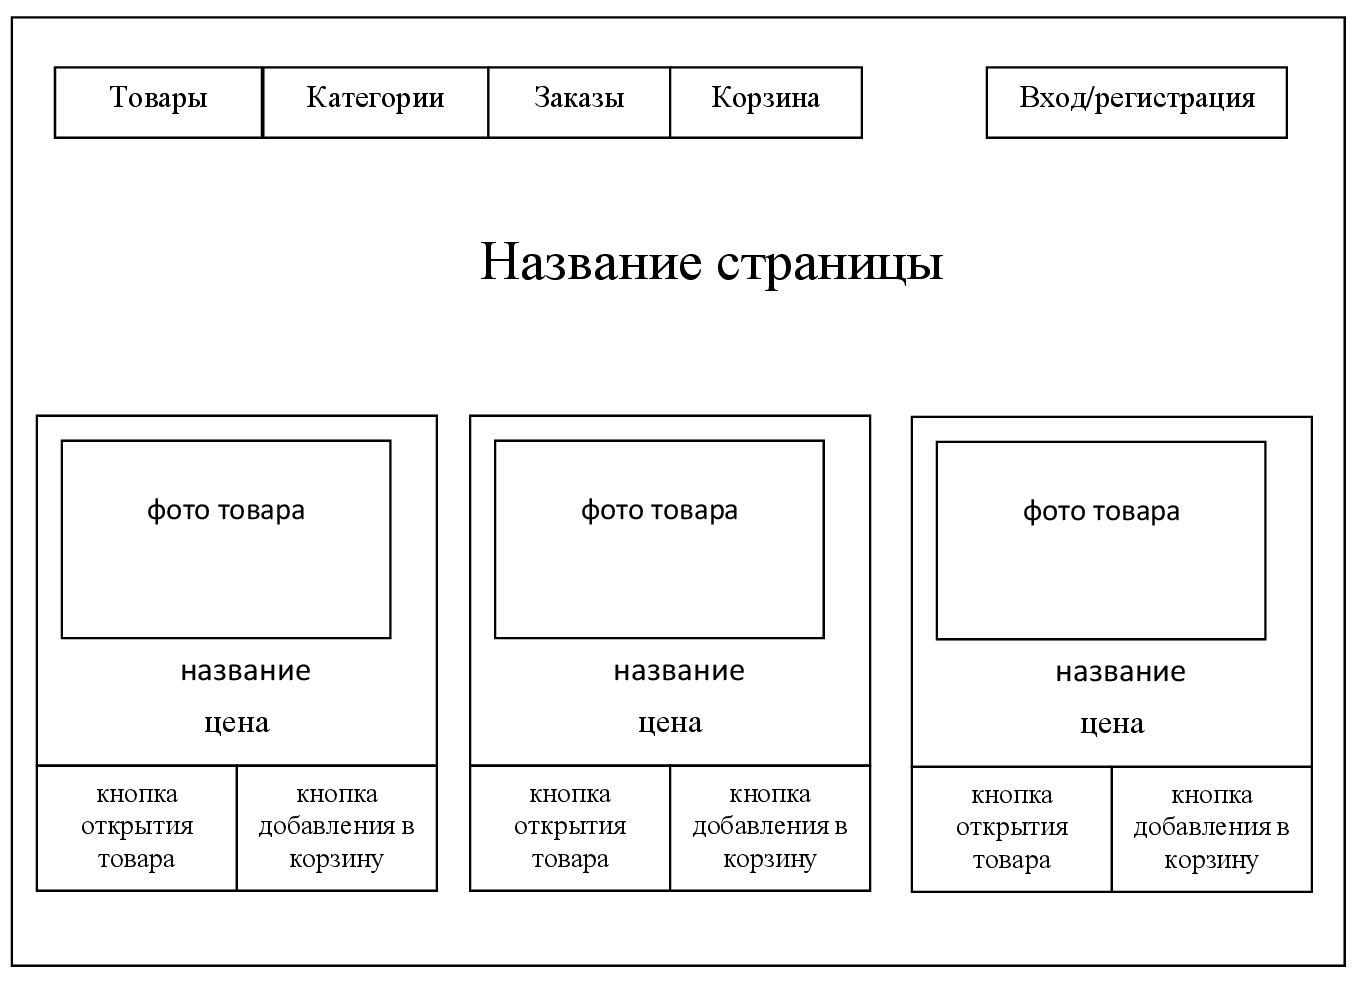
\includegraphics[width=1\linewidth]{interface}
	\caption{Макет страницы с товарами}
	\label{interface:image}
\end{figure}
%\vspace{-\figureaboveskip} % двойной отступ не нужен (можно использовать, если раздел заканчивается картинкой)

\subsubsection{Нефункциональные требования}

\paragraph{Требования к безопасности}
Необходимо устранить уязвимости, возможные для веб-приложений:
\begin{itemize}
	\item Межсайтовые скрипты (XSS) — это уязвимость системы безопасности, которая позволяет злоумышленнику размещать клиентские скрипты (обычно JavaScript) на веб-страницах. Когда другие пользователи загружают затронутые страницы, будут выполняться скрипты злоумышленника, что позволяет злоумышленнику украсть cookie-маркеры и маркеры сеанса, изменить содержимое веб-страницы с помощью DOM или перенаправить браузер на другую страницу.
	\item SQL-инъекция (Внедрение SQL-кода) — это попытка изменить запрос к базе данных. Ввести ее можно через форму или ссылку, которая передает параметры методом GET\cite{dronov}.
	\item Доступ обычного пользователя к возможностям администратора.
	\item Межсайтовая подделка запроса (CSRF) — это вид атак на сайт, при котором злоумышленник с помощью мошеннического сайта или скрипта заставляет браузер пользователя выполнять на доверенном сайте действия от его имени: отправлять сообщения, менять пароли, переводить деньги и пр. В атаке используются недостатки протокола HTTP. Чтобы стать жертвой, пользователю достаточно перейти по вредоносной ссылке.
\end{itemize}

\paragraph{Требования к программному обеспечению}
Для реализации программной системы необходимо подготовить следующие компоненты:
\begin{itemize}
	\item пакетный менеджер Composer для управления зависимостями;
	\item фреймворк Laravel;
	\item интерпретатор языка программирования PHP;
	\item СУБД MySQL;
	\item веб-сервер, поддерживающий PHP.
\end{itemize}

Laravel совместим со всеми современными операционными системами, включая Windows, macOS и Linux.

\paragraph{Требования к аппаратному обеспечению}
Для работы приложения требуется дисковое пространство не менее 2,5 Гб, минимум 2 Гб оперативной памяти и подключение к Интернету. Рекомендуется использовать процессор c 2 или более ядрами и частотой 2 ГГц или выше.

\subsection{Требования к оформлению документации}
Требования к стадиям разработки программ и программной документации для вычислительных машин, комплексов и систем независимо от их назначения и области применения, этапам и содержанию работ устанавливаются ГОСТ 19.102–77. 
Программная документация должна включать в себя: 
\begin{enumerate}
	\item Анализ предметной области.
	\item Техническое задание.
	\item Технический проект.
	\item Рабочий проект.
\end{enumerate}

\section{Технический проект}

\subsection{Выбор технологии проектирования}
\subsubsection{Паттерн MVC}
MVC (Model-View-Controller) - это схема разделения данных приложения и управляющей логики на три части:
\begin{itemize}
	\item модель (model) предоставляет данные и методы работы с ними: запросы в базу данных, проверка на корректность;
	\item представление (view) показывает пользователю эти данные;
	\item контроллер (controller) -- связующее звено между моделью и представлением. Он принимает запросы от представления, обрабатывает их и передаёт необходимые данные модели. Затем контроллер получает ответ от модели и передаёт его представлению для визуализации.
\end{itemize}

\subsection{Выбор средств разработки}
\subsubsection{PHP}

PHP (Preprocessor Hypertext) — это язык программирования, который широко применяется для разработки веб-приложений и сайтов \cite{gizbert}. Он обладает рядом преимуществ, делающих его популярным среди разработчиков:
\begin{itemize}
	\item Простота изучения: PHP относительно легко понять и освоить, особенно если у пользователя уже есть базовые знания HTML. Это делает его привлекательным выбором для начинающих программистов.
	\item Широкая поддержка: PHP имеет большое сообщество разработчиков, которое обеспечивает широкую поддержку и доступ к множеству ресурсов для обучения и решения проблем.
	\item Гибкость: PHP позволяет легко интегрировать различные технологии, такие как базы данных, XML, JSON и другие веб-технологии.
	\item Оптимизация производительности: PHP предлагает множество инструментов для оптимизации производительности, включая кэширование, минификацию кода и многопоточность.
	\item Поддержка MVC (Model-View-Controller): PHP поддерживает архитектуру MVC, которая помогает организовать код и упрощает разработку и поддержку больших приложений.
	\item Интеграция с другими языками программирования: PHP может быть использован вместе с другими языками программирования, такими как JavaScript, Python и Ruby. Это позволяет разработчикам использовать лучшие практики и инструменты из разных языков.
	\item Поддержка фреймворков: Существует множество популярных PHP-фреймворков, таких как Laravel, Symfony, CodeIgniter и Yii, которые предоставляют дополнительные инструменты и структуры для ускорения разработки.
\end{itemize}

\subsubsection{MySQL}

MySQL - это одна из самых популярных систем управления базами данных (СУБД). Это программа, которая позволяет создавать и управлять базами данных реляционного типа с использованием языка стандартизированных запросов (SQL). MySQL отличается своей доступностью как по финансовой стороне, так и по уровню сложности. Она проста в управлении и имеет развитое сообщество пользователей \cite{brett}.

С практической точки зрения, система MySQL обладает рядом преимуществ:
\begin{itemize}
	\item высокая скорость работы благодаря отказу от некоторых стандартов языка;
	\item простая установка и интуитивно понятный интерфейс, что делает её доступной даже для новичков;
	\item отсутствие ограничений по количеству пользователей;
	\item гибкость за счёт открытого исходного кода;
	\item богатый выбор сторонних инструментов (плагинов), что позволяет настроить систему под конкретные потребности;
	\item поддержка больших таблиц, содержащих до 50 миллионов строк;
	\item высокий уровень безопасности;
	\item широкий функционал, который позволяет использовать систему в различных сферах.
\end{itemize}

Эта СУБД считается надежной и стабильной уже долгие годы. Она поддерживает разные виды таблиц, быстро выполняет команды и может быть модифицирована под индивидуальные нужды проекта.

\subsubsection{Фреймворк Laravel}

Laravel -- это фреймворк для разработки веб-приложений, который отличается элегантным и выразительным синтаксисом. Он упрощает решение таких распространённых задач, как аутентификация, маршрутизация, управление сессиями и кэширование. Отдельно стоит упомянуть кэширование: благодаря соответствующему драйверу файловая система сохраняет в себе большое количество различных элементов. Подобный подход способствует более быстрой разработке самых разных по сложности приложений. В Laravel  также имеется удобная система аутентификации, с помощью которой можно контролировать доступ к имеющимся ресурсам.

Другие особенности платформы:
\begin{itemize}
	\item Встроенный ORM (Object-Relational Mapping). ORM -- это технология программирования для связи базы данных и языка программирования. Использование ORM позволяет ускорить разработку. Для PHP существует множество реализаций ORM, но Laravel пользуется собственной. Она называется Eloquent и работает по схеме ActiveRecord, согласно которой каждой таблице в базе данных соответствует один класс. Eloquent позволяет писать понятный код, который легко поддерживать, и предоставляет защиту от SQL-инъекций.
	\item Шаблонизатор Blade. Шаблонизаторы используются для превращения HTML-шаблонов в готовые страницы. Шаблоны -- это заготовки для будущих веб-страниц, которые включают HTML-верстку без контента и PHP-код. Задача программы-шаблонизатора -- выполнить PHP-код и подставить в шаблон контент, чтобы превратить его в готовую страницу. Blade -- это шаблонизатор фреймворка Laravel. Он не имеет ограничений на чистый PHP в шаблонах -- это удобнее для backend-разработчика.
	\item Консоль Artisan. Artisan -- интерфейс командной строки, включенный в Lavarel. Он позволяет генерировать модели, новые тесты, контроллеры, уведомления из командной строки. Это гораздо удобнее, чем копировать шаблоны классов или писать их вручную.
	\item Эффективная работа с трафиком. Чем известнее сайт, тем большее число запросов в секунду он должен обрабатывать. При большой нагрузке сервер иногда может не отвечать, и данные могут потеряться. Но подобные риски с Laravel сведены к минимуму благодаря интересной системе информационной очереди. С её помощью нагрузка на сервер упорядочивается.
\end{itemize}

\subsubsection{Blade}

Для разработки представлений был выбран язык шаблонизатора Blade. По сравнению с PHP, использование Blade позволяет делать код более чистым \cite{kirichenko}.

Преимущества Blade:
\begin{itemize}
	\item Простота использования. Для вывода данных достаточно использовать двойные фигурные скобки. Это позволяет избежать сложностей с выводом значений, экранированием строк и безопасностью.
	\item Безопасность. В отличие от PHP, где необходимо экранировать все выводимые данные, в Blade используются автоматические кавычки, что делает код более безопасным.
	\item Документированность. Blade хорошо документирован, что облегчает изучение и использование этого инструмента.
	\item Поддержка сообщества. Laravel имеет большое сообщество разработчиков, которые активно используют Blade и делятся своим опытом и решениями проблем.
	\item Расширяемость. Blade поддерживает пользовательские директивы, что позволяет расширять функциональность шаблонов без необходимости написания большого количества кода.
\end{itemize}

Выбор в пользу Blade добавляет дополнительный шаг в обработку шаблонов, т.к. все шаблоны Blade будут скомпилированы в PHP-код. Но благодаря кэшированию это не влияет на производительность приложения.

\subsection{Компоненты приложения}

\subsubsection{Сервис-провайдеры}

Сервис-провайдеры являются центральным местом начальной загрузки всех возможностей Laravel. Под загрузкой подразумевается регистрация нужных сервисов, включая регистрацию привязок к служебному контейнеру, прослушивателей событий, middleware и даже маршрутов.

Все классы сервис-провайдеров хранятся в config/app.php. Провайдеры, имеющиеся там изначально, загружают основные компоненты Laravel, такие как почтовый рассыльщик, очередь, кэш и другие. Многие из этих классов провайдеров являются «отложенными». Это означает, что они будут загружаться не при каждом запросе, а только при необходимости предоставляемых ими услуг. Пользователь может создавать собственные сервис-провайдеры для своего приложения.

Все сервис-провайдеры расширяют класс Illuminate/Support/ServiceProvider. Класс провайдера содержит 2 метода — register и boot. Метод register предназначен для привязки к сервисному контейнеру. Внутри любого из методов класса-провайдера всегда доступно свойство \$app, которое предоставляет доступ к сервисному контейнеру. Метод boot используется для расширения возможностей фреймворка, например, для создания новых blade-директив и запускается только после выполнения всех методов register.

\subsubsection{Сервис-контейнеры}

Сервис-контейнер или контейнер служб – это инструмент для управления зависимостями классов и выполнения внедрения зависимостей. Зависимости классов «вводятся» в класс через конструктор в виде аргументов или, в некоторых случаях, через методы-сеттеры. При создании класса или вызове методов фреймворк смотрит на список аргументов и, если нужно, создаёт экземпляры необходимых классов и сам подаёт их на вход конструктора или метода. 

Все контроллеры регистрируются через сервис-контейнер, поэтому при получении класса контроллера из контейнера автоматически получаются все зависимости, указанные в аргументах конструктора и других методах контроллера.


\subsubsection{Фасады}

Фасады предоставляют «статический» интерфейс для классов, доступных в сервис-контейнере приложения. Все фасады Laravel расширяют базовый класс Illuminate/Support/Facades/Facade. Базовый класс Facade использует магический метод \_\_callStatic(), чтобы делегировать вызовы из фасада объекту, извлеченному из контейнера.

Фасады предоставляют краткий и понятный синтаксис, который позволяет пользоваться функциями laravel без запоминания длинных названий классов, которые должны внедряться вручную. В дополнении к фасадам, Laravel предлагает множество глобальных вспомогательных функций, которые упрощают взаимодействие с общими функциями Laravel. Они доступны глобально и не требуют импортирования каких-либо классов для их использования. Многие вспомогательные функции выполняют те же задачи, что и соответствующие фасады.


\subsubsection{Результат проектирования}

Компоненты приложения и взамодействия между ними можно увидеть на диаграмме компонентов, приведённой на рисунке ~\ref{components:image}.
\begin{figure}[h!]
	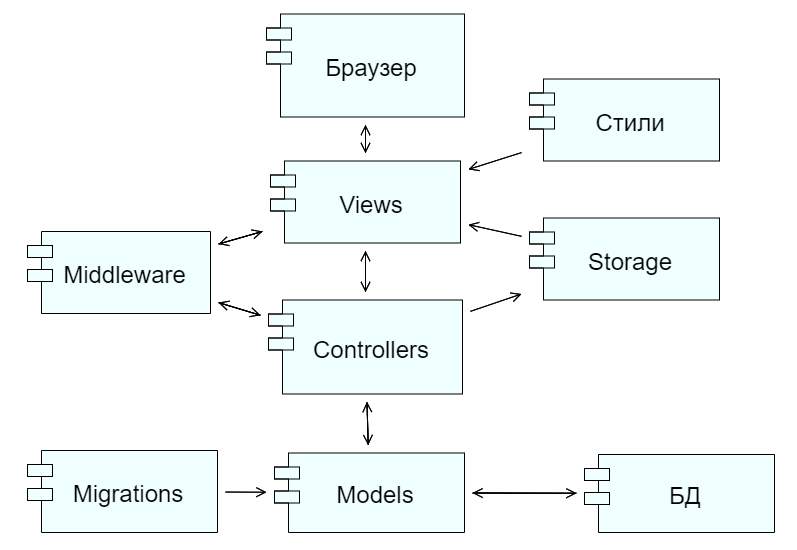
\includegraphics[width=0.8\linewidth]{components}
	\caption{Диаграмма компонентов приложения}
	\label{components:image}
\end{figure}
%\vspace{-\figureaboveskip} % двойной отступ не нужен (можно использовать, если раздел заканчивается картинкой)


\subsection{Структура каталогов}

Структура каталогов приложения включает следующие основные каталоги:
\begin{enumerate}
	\item App — содержит подкаталоги Console, Exceptions, Http, Models и Providers. Каталог Console содержит пользовательские команды Artisan. Каталог Exceptions содержит обработчик исключений. Каталог Http содержит контроллеры, middleware и запросы форм. Каталог Models содержит классы моделей Eloquent. Каталог Providers содержит сервис провайдеры, подготавливающие приложение к входящим запросам.
	\item Bootstrap — содержит файл app.php, загружающий фреймворк. Также в папке bootstrap находится папка cache, которая содержит сгенерированные фреймворком файлы для оптимизации производительности, например, кэш-файлы маршрутов и сервисов.
	\item Config — содержит файлы конфигурации приложения.
	\item Database — содержит миграции базы данных, фабрики моделей и данные для заполнения.
	\item Public — содержит index.php, являющийся точкой входа для всех запросов, поступающих в приложение, и ссылку на storage.
	\item Resources — содержит представления (view).
	\item Routes — содержит все определения маршрутов для приложения.
	\item Storage — разделён на подкаталоги storage/app, storage/framework и storage/logs. Каталог storage/framework используется для хранения кэшей. Storage/log хранит файлы журналов (логи) приложения. В каталоге storage/app/public хранятся изображения товаров.
	\item Tests — содержит автоматические тесты.
	\item Vendor — хранит зависимости, установленные через менеджер пакетов Composer. 
\end{enumerate}

\subsection{Структура базы данных}

В таблице \ref{bd:table} показана структура таблицы plant\_categories.

\begin{xltabular}{\textwidth}{|c|X|X|X|}
	\caption{\label{bd:table}Таблица plant\_categories} \\ \hline
	\thead {Тип ключа} & \thead {Обязательность} & \thead {Имя столбца}
	& \thead {Тип данных} \\ \hline
	\endfirsthead
	\continuecaption{Продолжение таблицы \ref{bd:table}}
	\thead {Тип ключа} & \thead {Обязательность} & \thead {Имя столбца}
	& \thead {Тип данных} \\ \hline
	\finishhead
	primary key & да & id & integer \\ \hline 
	~ & да &	name & string \\ \hline 
	~ & да &	description & text
\end{xltabular}


В таблице \ref{bd2:table} показана структура таблицы plant\_genera.

\begin{xltabular}{\textwidth}{|c|X|X|X|}
	\caption{Таблица plant\_genera\label{bd2:table}}\\ \hline
	\thead {Тип ключа} & \thead {Обязательность} & \thead {Имя столбца}
	& \thead {Тип данных} \\ \hline
	\endfirsthead
	\continuecaption{Продолжение таблицы \ref{bd2:table}}
	\thead {Тип ключа} & \thead {Обязательность} & \thead {Имя столбца}
	& \thead {Тип данных} \\ \hline
	\finishhead
	primary key & да & name & string \\ \hline 
	~ & да & description & text
\end{xltabular}

В таблице \ref{bd3:table} показана структура таблицы product\_types.

\begin{xltabular}{\textwidth}{|c|X|X|X|}
	\caption{Таблица product\_types\label{bd3:table}}\\ \hline
	\thead {Тип ключа} & \thead {Обязательность} & \thead {Имя столбца}
	& \thead {Тип данных} \\ \hline
	\endfirsthead
	\continuecaption{Продолжение таблицы \ref{bd3:table}}
	\thead {Тип ключа} & \thead {Обязательность} & \thead {Имя столбца}
	& \thead {Тип данных} \\ \hline
	\finishhead
	primary key & да & name & string
\end{xltabular}

В таблице \ref{bd4:table} показана структура таблицы plant\_colors.

\begin{xltabular}{\textwidth}{|c|X|X|X|}
	\caption{Таблица plant\_colors\label{bd4:table}}\\ \hline
	\thead {Тип ключа} & \thead {Обязательность} & \thead {Имя столбца}
	& \thead {Тип данных} \\ \hline
	\endfirsthead
	\continuecaption{Продолжение таблицы \ref{bd4:table}}
	\thead {Тип ключа} & \thead {Обязательность} & \thead {Имя столбца}
	& \thead {Тип данных} \\ \hline
	\finishhead
	primary key & да & name & string
\end{xltabular}

В таблице \ref{bd5:table} показана структура таблицы climate\_zones.

\begin{xltabular}{\textwidth}{|c|X|X|X|}
	\caption{Таблица climate\_zones\label{bd5:table}}\\ \hline
	\thead {Тип ключа} & \thead {Обязательность} & \thead {Имя столбца}
	& \thead {Тип данных} \\ \hline
	\endfirsthead
	\continuecaption{Продолжение таблицы \ref{bd5:table}}
	\thead {Тип ключа} & \thead {Обязательность} & \thead {Имя столбца}
	& \thead {Тип данных} \\ \hline
	\finishhead
	primary key & да & zone\_number & integer \\ \hline 
	~ & да & lower\_temp\_limit & integer \\ \hline 
	~ & да & upper\_temp\_limit & integer
\end{xltabular}

В таблице \ref{bd6:table} показана структура таблицы light\_modes.

\begin{xltabular}{\textwidth}{|c|X|X|X|}
	\caption{Таблица light\_modes\label{bd6:table}}\\ \hline
	\thead {Тип ключа} & \thead {Обязательность} & \thead {Имя столбца}
	& \thead {Тип данных} \\ \hline
	\endfirsthead
	\continuecaption{Продолжение таблицы \ref{bd6:table}}
	\thead {Тип ключа} & \thead {Обязательность} & \thead {Имя столбца}
	& \thead {Тип данных} \\ \hline
	\finishhead
	primary key & да & name & string
\end{xltabular}

В таблице \ref{bd7:table} показана структура таблицы soils.

\begin{xltabular}{\textwidth}{|c|X|X|X|}
	\caption{Таблица soils\label{bd7:table}}\\ \hline
	\thead {Тип ключа} & \thead {Обязательность} & \thead {Имя столбца}
	& \thead {Тип данных} \\ \hline
	\endfirsthead
	\continuecaption{Продолжение таблицы \ref{bd7:table}}
	\thead {Тип ключа} & \thead {Обязательность} & \thead {Имя столбца}
	& \thead {Тип данных} \\ \hline
	\finishhead
	primary key & да & name & string
\end{xltabular}

В таблице \ref{bd8:table} показана структура таблицы life\_cycles.

\begin{xltabular}{\textwidth}{|c|X|X|X|}
	\caption{Таблица life\_cycles\label{bd8:table}}\\ \hline
	\thead {Тип ключа} & \thead {Обязательность} & \thead {Имя столбца}
	& \thead {Тип данных} \\ \hline
	\endfirsthead
	\continuecaption{Продолжение таблицы \ref{bd8:table}}
	\thead {Тип ключа} & \thead {Обязательность} & \thead {Имя столбца}
	& \thead {Тип данных} \\ \hline
	\finishhead
	primary key & да & name & string
\end{xltabular}

В таблице \ref{bd9:table} показана структура таблицы plants.

\begin{xltabular}{\textwidth}{|c|X|X|X|}
	\caption{Таблица plants\label{bd9:table}}\\ \hline
	\thead {Тип ключа} & \thead {Обязательность} & \thead {Имя столбца}
	& \thead {Тип данных} \\ \hline
	\endfirsthead
	\continuecaption{Продолжение таблицы \ref{bd9:table}}
	\thead {Тип ключа} & \thead {Обязательность} & \thead {Имя столбца}
	& \thead {Тип данных} \\ \hline
	\finishhead
	primary key & да & id & integer \\ \hline
	~ & да & name & string \\ \hline
	~ & да & description & text \\ \hline
	~ & да & quantity & integer \\ \hline
	~ & да & price & decimal \\ \hline
	~ & нет & image & text \\ \hline
	~ & да & flower\_diameter & decimal \\ \hline
	foreign key & да & genus & string \\ \hline
	foreign key & да & product\_type & string \\ \hline
	foreign key & да & life\_cycle & string \\ \hline
	foreign key & да & soil & string \\ \hline
	foreign key & да & landing\_place & string \\ \hline
	foreign key & да & climate\_zone & integer \\ \hline
	foreign key & да & flower\_color1 & string \\ \hline
	foreign key & нет & flower\_color2 & string \\ \hline
	foreign key & нет & flower\_color3 & string \\ \hline
	foreign key & да & leaf\_color1 & string \\ \hline
	foreign key & нет & leaf\_color2 & string \\ \hline
	foreign key & нет & leaf\_color3 & string
\end{xltabular}

В таблице \ref{bd10:table} показана структура таблицы users.

\begin{xltabular}{\textwidth}{|c|X|X|X|}
	\caption{Таблица users\label{bd10:table}}\\ \hline
	\thead {Тип ключа} & \thead {Обязательность} & \thead {Имя столбца}
	& \thead {Тип данных} \\ \hline
	\endfirsthead
	\continuecaption{Продолжение таблицы \ref{bd10:table}}
	\thead {Тип ключа} & \thead {Обязательность} & \thead {Имя столбца}
	& \thead {Тип данных} \\ \hline
	\finishhead
	primary key & да & id & integer \\ \hline
	~ & да & name & string \\ \hline
	~ & да & email & string \\ \hline
	~ & нет & email\_verified\_at & timestamp \\ \hline
	~ & да & password & string \\ \hline
	~ & да & is\_admin & tinyInteger
\end{xltabular}

В таблице \ref{bd11:table} показана структура таблицы orders.

\begin{xltabular}{\textwidth}{|c|X|X|X|}
	\caption{Таблица orders\label{bd11:table}}\\ \hline
	\thead {Тип ключа} & \thead {Обязательность} & \thead {Имя столбца}
	& \thead {Тип данных} \\ \hline
	\endfirsthead
	\continuecaption{Продолжение таблицы \ref{bd11:table}}
	\thead {Тип ключа} & \thead {Обязательность} & \thead {Имя столбца}
	& \thead {Тип данных} \\ \hline
	\finishhead
	primary key & да & id & integer \\ \hline
	~ & да & status & integer \\ \hline
	~ & нет & name & text \\ \hline
	~ & нет & phone & text \\ \hline
	~ & нет & address & text \\ \hline
	~ & нет & email & string \\ \hline
	foreign key & нет & user\_id & integer
\end{xltabular}

В таблице \ref{bd12:table} показана структура таблицы order\_plant.

\begin{xltabular}{\textwidth}{|c|X|X|X|}
	\caption{Таблица order\_plant\label{bd12:table}}\\ \hline
	\thead {Тип ключа} & \thead {Обязательность} & \thead {Имя столбца}
	& \thead {Тип данных} \\ \hline
	\endfirsthead
	\continuecaption{Продолжение таблицы \ref{bd12:table}}
	\thead {Тип ключа} & \thead {Обязательность} & \thead {Имя столбца}
	& \thead {Тип данных} \\ \hline
	\finishhead
	primary key & да & id & integer \\ \hline
	~ & да & plant\_count & integer \\ \hline
	foreign key & да & order\_id  & integer \\ \hline
	foreign key & да & plant\_id & integer
\end{xltabular}

В таблице \ref{bd13:table} показана структура таблицы plant\_plant\_category.

\begin{xltabular}{\textwidth}{|c|X|X|X|}
	\caption{Таблица plant\_plant\_category\label{bd13:table}}\\ \hline
	\thead {Тип ключа} & \thead {Обязательность} & \thead {Имя столбца}
	& \thead {Тип данных} \\ \hline
	\endfirsthead
	\continuecaption{Продолжение таблицы \ref{bd13:table}}
	\thead {Тип ключа} & \thead {Обязательность} & \thead {Имя столбца}
	& \thead {Тип данных} \\ \hline
	\finishhead
	primary key & да & id & integer \\ \hline
	foreign key & да & plant\_category\_id   & integer \\ \hline
	foreign key & да & plant\_id & integer
\end{xltabular}

\subsection{Список контроллеров}

Каталог Controller содержит следующие контроллеры: 
\begin{itemize}
	\item Controller – родительский контроллер для остальных контроллеров;
	\item MainController – отвечает за отображение некоторых страниц, в том числе главной страницы сайта;
	\item HomeController – отвечает за отображение заказов пользователя;
	\item BasketController – отвечает за добавление товара в корзину и отображение корзины.
\end{itemize}

Каталог Controller также содержит подкаталоги Admin и Auth.

\subsubsection{Контроллеры подкаталога Admin}
Подкаталог Admin предназначен для контроллеров, предоставляющих методы для администратора сайта:
\begin{itemize}
	\item CategoryController – ресурсный контроллер для управления категориями;
	\item OrderController – отвечает за отображение заказов у администратора;
	\item PlantController – ресурсный контроллер для управления товарами.
\end{itemize}

\subsubsection{Контроллеры подкаталога Auth}
Подкаталог Auth объединяет контроллеры для регистрации и авторизации: 
\begin{itemize}
	\item ConfirmPasswordController – предназначен для обработки подтверждения пароля;
	\item ForgotPasswordController – отвечает за отправку электронных писем для сброса пароля;
	\item LoginController – обрабатывает аутентификацию ;
	\item RegisterController – обрабатывает регистрацию новых пользователей;
	\item ResetPasswordController – содержит логику сброса пароля;
	\item VerificationController – отвечает за переход пользователей на другую страницу после верификации.
\end{itemize}

\subsection{Список представлений}

Каталог views содержит подкаталоги frontend, orders, auth, layouts и admin.

\subsubsection{Представления подкаталога frontend}
Подкаталог frontend содержит страницы для просмотра и заказа товаров:
\begin{itemize}
	\item index.blade.php – главная страница со всеми товарами;
	\item categories.blade.php – страница категорий товаров;
	\item category.blade.php – страница категории;
	\item product.blade.php – страница товара;
	\item basket.blade.php – корзина;
	\item order.blade.php – страница оформления заказа;
\end{itemize}

\subsubsection{Представления подкаталога orders}
Подкаталог orders содержит страницы заказов пользователя:
\begin{itemize}
	\item home.blade.php – страница заказов;
	\item order.blade.php – страница заказа.
\end{itemize}

\subsubsection{Представления подкаталога auth}
Подкаталог auth содержит страницы авторизации и регистрации:
\begin{itemize}
	\item login.blade.php – страница аутентификации;
	\item register.blade.php – страница регистрации;
	\item verify.blade.php – страница верификации;
\end{itemize}

В этом подкаталоге также есть раздел passwords, объединяющий страницы для пароля:
\begin{itemize}
	\item confirm.blade.php – форма для подтверждения пароля;
	\item email.blade.php – форма для ввода адреса электронной почты для сброса пароля;
	\item reset.blade.php – форма для создания нового пароля.
\end{itemize}

\subsubsection{Представления подкаталога layouts}
Подкаталог layouts содержит представления, используемые другими представлениями:
\begin{itemize}
	\item master.blade.php – HTML-каркас для других представлений с подключёнными стилями и меню;
	\item card.blade.php – шаблон карточки товара;
	\item filters.blade.php – поле выбора характеристик, по которым можно отфильтровать товары.
\end{itemize}

\subsubsection{Представления подкаталога admin}
Подкаталог admin делится на разделы categories, orders и plants. 

Раздел categories содержит страницы для работы с категориями:
\begin{itemize}
	\item index.blade.php – страница категорий;
	\item show.blade.php – страница категории;
	\item form.blade.php – страница добавления или редактирования категории.
\end{itemize}

Раздел orders содержит страницы для просмотра заказов:
\begin{itemize}
	\item index.blade.php – страница заказов;
	\item show.blade.php – страница заказа;
\end{itemize}

Раздел plants содержит страницы для работы с товарами:
\begin{itemize}
	\item index.blade.php – страница товаров;
	\item show.blade.php – страница товара;
	\item form.blade.php – страница добавления или редактирования товара.
\end{itemize}

\subsection{Стили приложения}
Стили приложения можно найти по пути public/assets/css. Они представлены двумя файлами: bootstrap.min.css и starter-template.css. Эти стили подключаются в представлении layouts/master.blade.php. Файл bootstrap.min.css позволяет использовать возможности фреймворка Bootstrap для стилизации контента с помощью отдельных классов и компонентов. Одна из ключевых особенностей фреймворка – использование сетки, которая позволяет легко управлять распределением контента на разных размерах экранов.

\ifПрактика{}\else{
   \section{Рабочий проект}
\subsection{Маршруты приложения}
В таблице \ref{routes:table} показаны маршруты приложения.

\begin{small}
\begin{xltabular}{\textwidth}{|X|c|c|}
	\caption{\label{routes:table}Маршруты приложения} \\ \hline
	\thead {URI} & \thead {HTTP-метод} & \thead {Метод контроллера} \\ \hline
	\endfirsthead
	\continuecaption{Продолжение таблицы \ref{routes:table}}
	\thead {URI} & \thead {HTTP-метод} & \thead {Метод контроллера} \\ \hline
	\finishhead
	/ & GET|HEAD & MainController@Index \\ \hline
	/admin/categories & GET|HEAD & Admin/CategoryController@index \\ \hline
	/admin/categories & POST & Admin/CategoryController@store \\ \hline
	/admin/categories/create  & GET|HEAD & Admin/CategoryController@create\\ \hline
	/admin/categories/ \{category\}  & GET|HEAD & Admin/CategoryController@show \\ \hline
	/admin/categories/ \{category\} & PUT|PATCH & Admin/CategoryController@update \\ \hline
	/admin/categories/ \{category\} & DELETE & Admin/CategoryController@destroy \\ \hline
	/admin/categories/ \{category\}/edit & GET|HEAD & Admin/CategoryController@edit \\ \hline
	/admin/orders  & GET|HEAD & Admin/OrderController@index \\ \hline
	/admin/orders/\{order\}  & GET|HEAD & Admin/OrderController@show \\ \hline
	/admin/ plants & GET|HEAD & Admin/PlantController@index \\ \hline
	/admin/ plants & POST & Admin/PlantController@store \\ \hline
	/admin/plants/create  & GET|HEAD & Admin/PlantController@create\\ \hline
	/admin/plants/\{plant\}  & GET|HEAD & Admin/PlantController@show  \\ \hline
	/admin/plants/\{plant\}  & PUT|PATCH & Admin/PlantController@update \\ \hline
	/admin/plants/\{plant\} & DELETE & Admin/PlantController@destroy \\ \hline
	/admin/plants/\{plant\}/edit & GET|HEAD & Admin/PlantController@edit   \\ \hline
	/basket & GET|HEAD & BasketController@basket \\ \hline
	/basket/add/\{id\}& POST & BasketController@basketAdd \\ \hline
	/basket/place & GET|HEAD & BasketController@basketPlace \\ \hline
	/basket/place & POST & BasketController@basketConfirm  \\ \hline
	/basket/remove/\{id\}& POST & BasketController@basketRemove \\ \hline
	/categories & GET|HEAD & MainController@categories  \\ \hline
	/categories/\{category\}& GET|HEAD & MainController@category \\ \hline
	/products/\{product\}& GET|HEAD & MainController@product \\ \hline
	/home & GET|HEAD & HomeController@index \\ \hline
	/home/\{order\} & GET|HEAD & HomeController@order \\ \hline
	/login & GET|HEAD & Auth/LoginController@showLoginForm  \\ \hline
	/login & POST & Auth/LoginController@login  \\ \hline
	/logout & POST & Auth/LoginController@logout  \\ \hline
	/logout & GET|HEAD & Auth/LoginController@logout  \\ \hline
	/password/confirm & GET|HEAD & Auth/ConfirmPasswordController@showConfirmForm  \\ \hline
	/password/confirm & POST & Auth/ConfirmPasswordController@confirm  \\ \hline
	/password/email & POST & Auth/ForgotPasswordController@sendResetLinkEmail \\ \hline
	/password/reset & GET|HEAD & Auth/ForgotPasswordController@showLinkRequestForm  \\ \hline
	/password/reset & POST & Auth/ResetPasswordController@reset  \\ \hline
	/password/reset/\{token\} & GET|HEAD & Auth/ResetPasswordController@showResetForm  \\ \hline
	/register & GET|HEAD & Auth/RegisterController@showRegistrationForm  \\ \hline
	/register & POST & Auth/RegisterController@register  \\ \hline
	/admin/categories & GET|HEAD & Admin/CategoryController@index 
\end{xltabular}
\end{small}


\subsection{Спецификация контроллеров приложения}

В таблице \ref{contr1:table} приведено описание методов класса <<MainController>>.

\begin{xltabular}{\textwidth}{|c|c|X|}
	\caption{\label{contr1:table}Спецификация методов класса <<MainController>>} \\ \hline
	\thead {Название} & \thead {Доступ} & \thead {Описание}\\ \hline
	\endfirsthead
	\continuecaption{Продолжение таблицы \ref{contr1:table}}
	\thead {Название} & \thead {Доступ} & \thead {Описание}\\ \hline
	\finishhead
	index & public & Выводит представление для главной страницы \\ \hline 
	categories & public & Выводит представление для категорий \\ \hline 
	category & public & Выводит представление для категории \\ \hline
	product & public & Выводит представление для товара
\end{xltabular}


В таблице \ref{contr2:table} приведено описание методов класса <<HomeController>>.

\begin{xltabular}{\textwidth}{|c|c|X|}
	\caption{\label{contr2:table}Спецификация методов класса <<HomeController>>} \\ \hline
	\thead {Название} & \thead {Доступ} & \thead {Описание}\\ \hline
	\endfirsthead
	\continuecaption{Продолжение таблицы \ref{contr2:table}}
	\thead {Название} & \thead {Доступ} & \thead {Описание}\\ \hline
	\finishhead
	\_\_construct & public & Устанавливает доступ только для зарегистрированных пользователей \\ \hline 
	index & public & Выводит представление для заказов пользователя\\ \hline 
	order & public & Выводит представление для заказа пользователя
\end{xltabular}


В таблице \ref{contr3:table} приведено описание методов класса <<BasketController>>.

\begin{xltabular}{\textwidth}{|c|c|X|}
	\caption{\label{contr3:table}Спецификация методов класса <<BasketController>>} \\ \hline
	\thead {Название} & \thead {Доступ} & \thead {Описание}\\ \hline
	\endfirsthead
	\continuecaption{Продолжение таблицы \ref{contr3:table}}
	\thead {Название} & \thead {Доступ} & \thead {Описание}\\ \hline
	\finishhead
	basket & public & Выводит представление для корзины \\ \hline 
	basketPlace & public & Выводит представление для оформления заказа \\ \hline
	basketConfirm & public & Сохраняет данные заказа и переносит пользователя на главную страницу после оформления заказа \\ \hline 
	basketAdd & public & Добавляет товар в корзину \\ \hline
	basketRemove & public & Удаляет товар из корзины
\end{xltabular}


Далее будет представлена спецификация контроллеров, находящихся в папке <<Admin>>.

В таблице \ref{contr4:table} приведено описание методов класса <<CategoryController>>.

\begin{xltabular}{\textwidth}{|c|c|X|}
	\caption{\label{contr4:table}Спецификация методов класса <<CategoryController>>} \\ \hline
	\thead {Название} & \thead {Доступ} & \thead {Описание}\\ \hline
	\endfirsthead
	\continuecaption{Продолжение таблицы \ref{contr4:table}}
	\thead {Название} & \thead {Доступ} & \thead {Описание}\\ \hline
	\finishhead
	index & public & Выводит представление для категорий в панели администратора \\ \hline 
	create & public & Выводит представление для создания категории \\ \hline 
	store & public & Сохраняет категорию в базу данных \\ \hline
	show & public & Выводит представление для категории в панели администратора \\ \hline
	edit & public & Выводит представление для редактирования категории \\ \hline
	update & public & Обновляет информацию о категории в базе данных \\ \hline
	destroy & public & Удаляет категорию из базы данных
\end{xltabular}


В таблице \ref{contr5:table} приведено описание методов класса <<OrderController>>.

\begin{xltabular}{\textwidth}{|c|c|X|}
	\caption{\label{contr5:table}Спецификация методов класса <<OrderController>>} \\ \hline
	\thead {Название} & \thead {Доступ} & \thead {Описание}\\ \hline
	\endfirsthead
	\continuecaption{Продолжение таблицы \ref{contr5:table}}
	\thead {Название} & \thead {Доступ} & \thead {Описание}\\ \hline
	\finishhead
	index & public & Выводит представление для заказов в панели администратора \\ \hline 
	show & public & Выводит представление для заказа в панели администратора 
\end{xltabular}


В таблице \ref{contr6:table} приведено описание методов класса <<PlantController>>.

\begin{xltabular}{\textwidth}{|c|c|X|}
	\caption{\label{contr6:table}Спецификация методов класса <<PlantController>>} \\ \hline
	\thead {Название} & \thead {Доступ} & \thead {Описание}\\ \hline
	\endfirsthead
	\continuecaption{Продолжение таблицы \ref{contr6:table}}
	\thead {Название} & \thead {Доступ} & \thead {Описание}\\ \hline
	\finishhead
	index & public & Выводит представление для товаров в панели администратора \\ \hline 
	create & public & Выводит представление для создания товара \\ \hline 
	store & public & Сохраняет товар в базу данных \\ \hline
	show & public & Выводит представление для товара в панели администратора \\ \hline
	edit & public & Выводит представление для редактирования товара \\ \hline
	update & public & Обновляет информацию о товаре в базе данных \\ \hline
	destroy & public & Удаляет товар из базы данных
\end{xltabular}



Далее будет представлена спецификация контроллеров, находящихся в папке <<Auth>>.

В таблице \ref{contr7:table} приведено описание методов класса <<ConfirmPasswordController>>.

\begin{xltabular}{\textwidth}{|c|c|X|}
	\caption{\label{contr7:table}Спецификация методов класса <<ConfirmPasswordController>>} \\ \hline
	\thead {Название} & \thead {Доступ} & \thead {Описание}\\ \hline
	\endfirsthead
	\continuecaption{Продолжение таблицы \ref{contr7:table}}
	\thead {Название} & \thead {Доступ} & \thead {Описание}\\ \hline
	\finishhead
	\_\_construct & public & Разрешает доступ только авторизованным пользователям
\end{xltabular}


В таблице \ref{contr8:table} приведено описание методов класса <<LoginController>>.

\begin{xltabular}{\textwidth}{|c|c|X|}
	\caption{\label{contr8:table}Спецификация методов класса <<LoginController>>} \\ \hline
	\thead {Название} & \thead {Доступ} & \thead {Описание}\\ \hline
	\endfirsthead
	\continuecaption{Продолжение таблицы \ref{contr8:table}}
	\thead {Название} & \thead {Доступ} & \thead {Описание}\\ \hline
	\finishhead
	redirectTo & protected & Переносит пользователя на другую страницу после входа \\ \hline 
	\_\_construct & public & Разрешает доступ только неавторизованным пользователям 
\end{xltabular}


В таблице \ref{contr9:table} приведено описание методов класса <<RegisterController>>.

\begin{xltabular}{\textwidth}{|c|c|X|}
	\caption{\label{contr9:table}Спецификация методов класса <<RegisterController>>} \\ \hline
	\thead {Название} & \thead {Доступ} & \thead {Описание}\\ \hline
	\endfirsthead
	\continuecaption{Продолжение таблицы \ref{contr9:table}}
	\thead {Название} & \thead {Доступ} & \thead {Описание}\\ \hline
	\finishhead
	redirectTo & protected & Переносит пользователя на другую страницу после регистрации \\ \hline 
	\_\_construct & public & Разрешает доступ только неавторизованным пользователям \\ \hline 
	validator & protected & Валидирует данные для регистрации пользователя \\ \hline
	create & protected & Сохраняет нового пользователя в базе данных
\end{xltabular}


В таблице \ref{contr10:table} приведено описание методов класса <<ResetPasswordController>>.

\begin{xltabular}{\textwidth}{|c|c|X|}
	\caption{\label{contr10:table}Спецификация методов класса <<ResetPasswordController>>} \\ \hline
	\thead {Название} & \thead {Доступ} & \thead {Описание}\\ \hline
	\endfirsthead
	\continuecaption{Продолжение таблицы \ref{contr10:table}}
	\thead {Название} & \thead {Доступ} & \thead {Описание}\\ \hline
	\finishhead
	redirectTo & protected & Переносит пользователя на другую страницу после сброса пароля \\ \hline
\end{xltabular}


В таблице \ref{contr11:table} приведено описание методов класса <<VerificationController>>.

\begin{xltabular}{\textwidth}{|c|c|X|}
	\caption{\label{contr11:table}Спецификация методов класса <<VerificationController>>} \\ \hline
	\thead {Название} & \thead {Доступ} & \thead {Описание}\\ \hline
	\endfirsthead
	\continuecaption{Продолжение таблицы \ref{contr11:table}}
	\thead {Название} & \thead {Доступ} & \thead {Описание}\\ \hline
	\finishhead
	redirectTo & protected & Переносит пользователя на другую страницу после верификации \\ \hline 
	\_\_construct & public & Разрешает доступ только авторизованным пользователям \\ \hline 
\end{xltabular}


\subsection{Системное тестирование разработанного web-сайта}

На рисунке \ref{index:image} показана главная страница сайта.

\begin{figure}[H]
	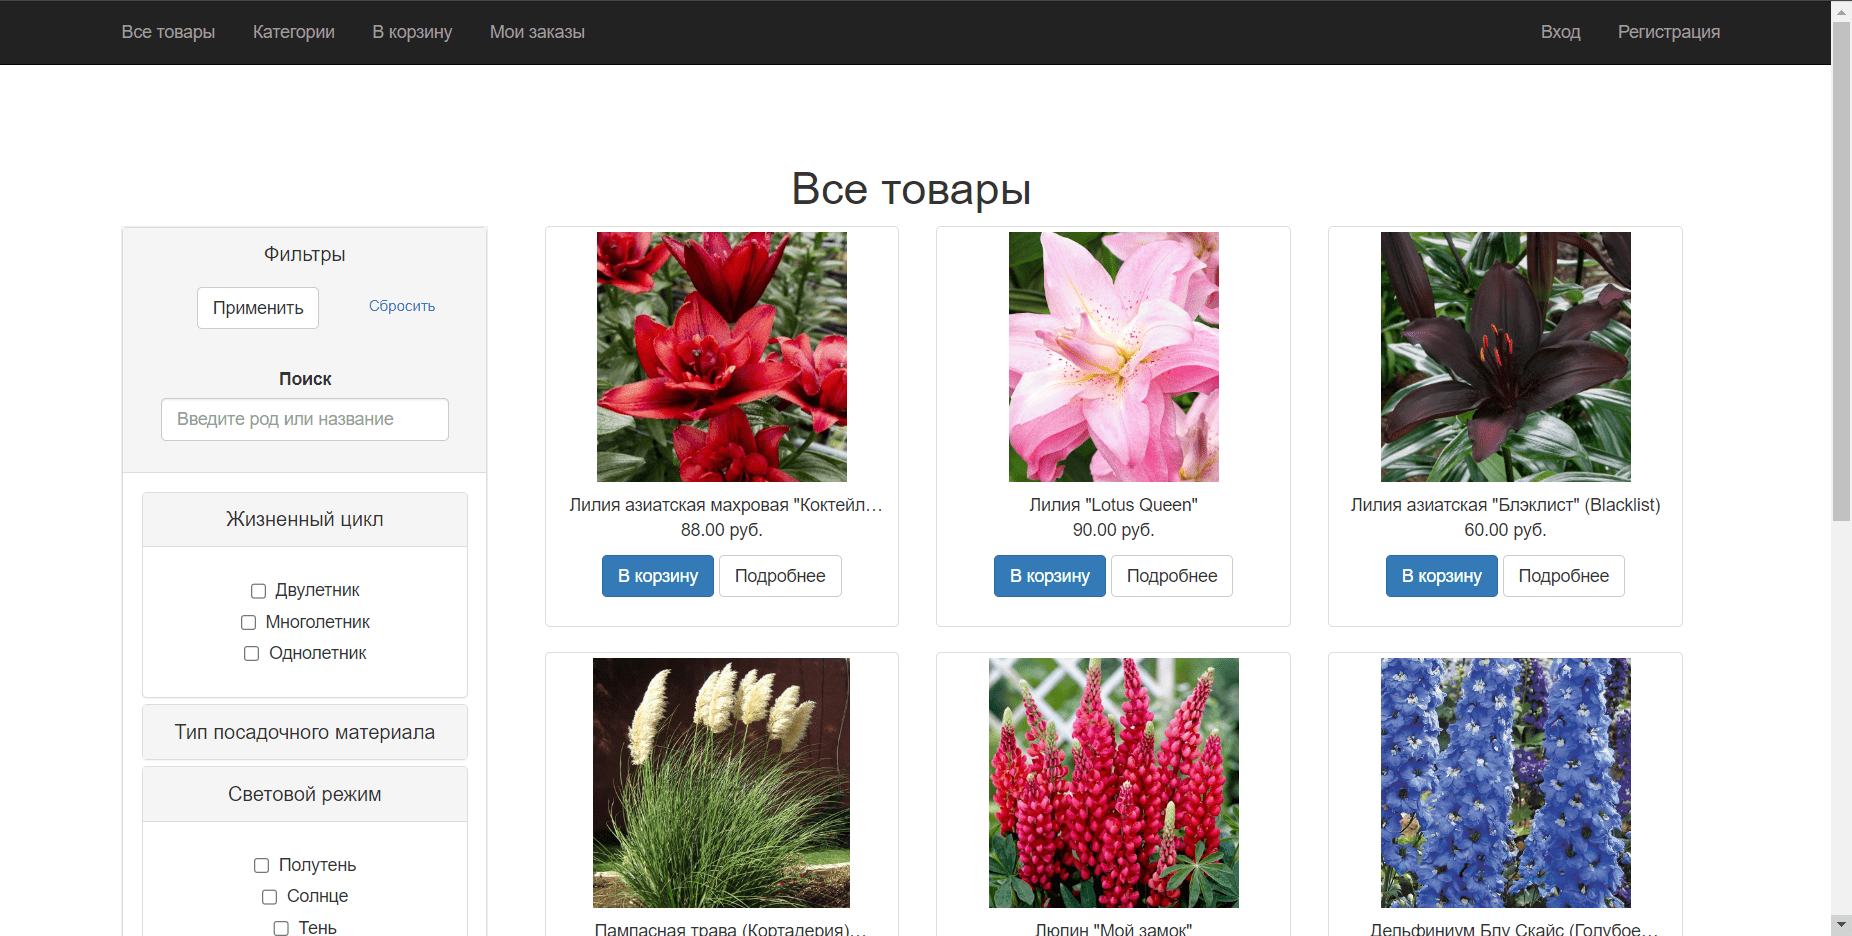
\includegraphics[width=1\linewidth]{index}
	\caption{Главная страница}
	\label{index:image}
\end{figure}
%\vspace{-\figureaboveskip} % двойной отступ не нужен (можно использовать, если раздел заканчивается картинкой)

На рисунке \ref{1filter:image} показан результат фильтрации товаров на главной странице по одному параметру.

\begin{figure}[H]
	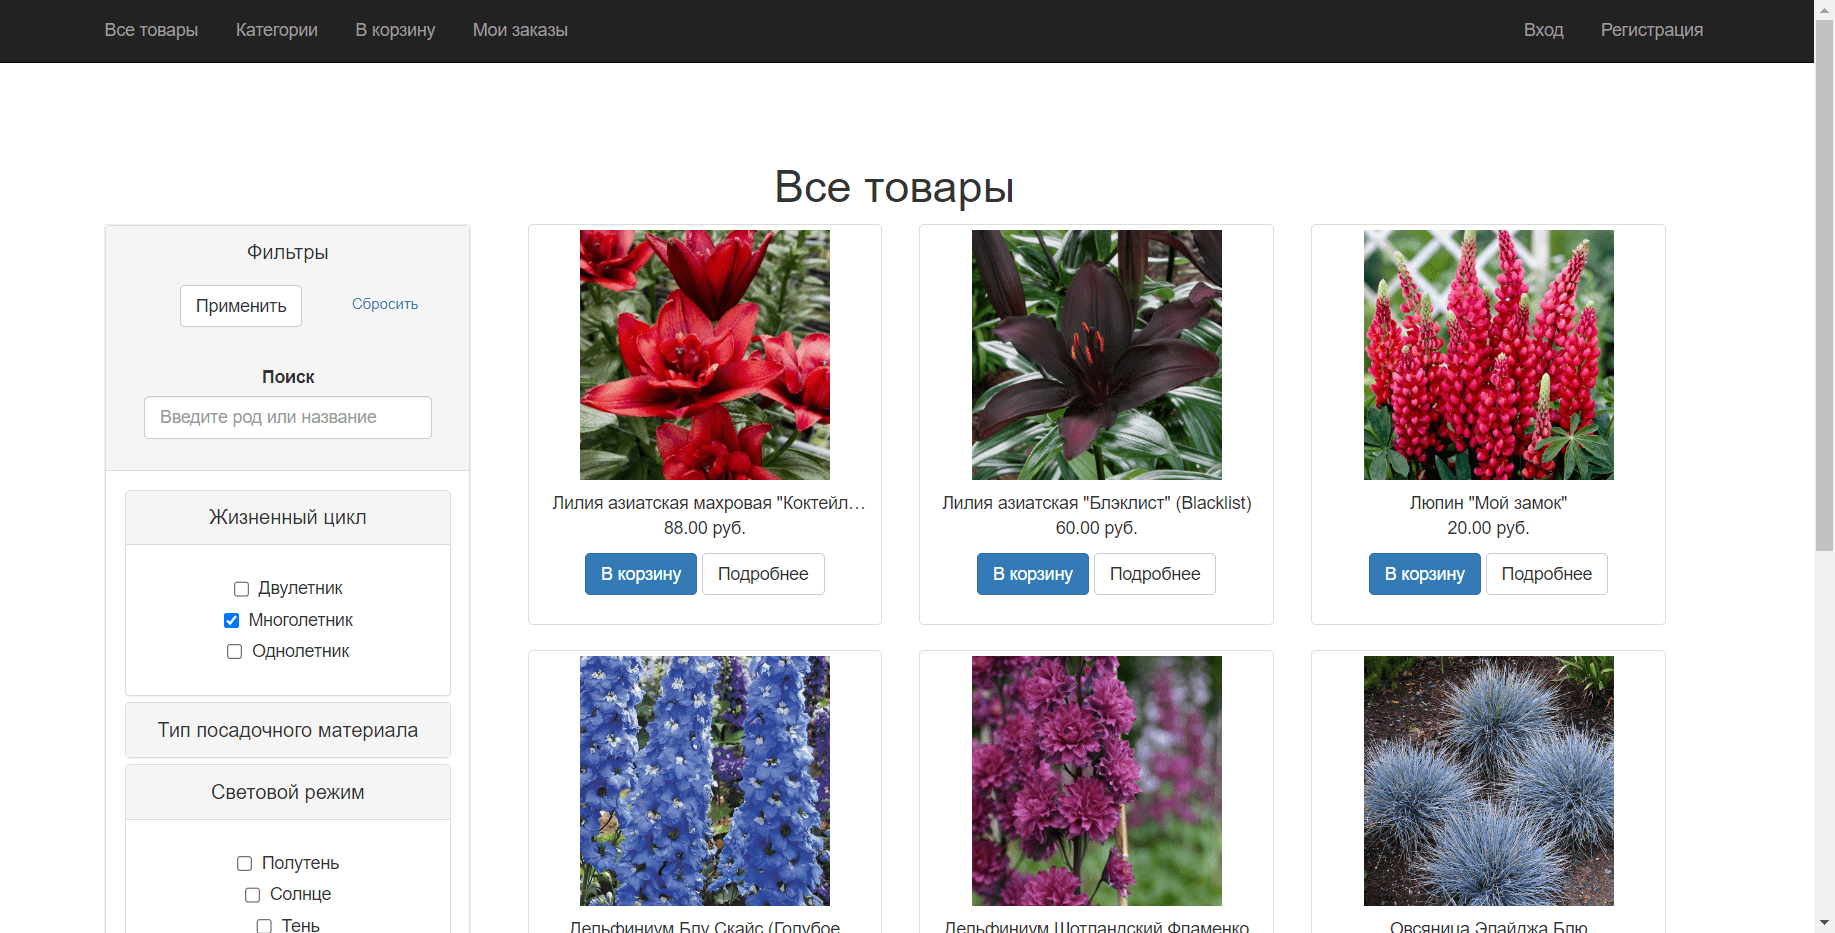
\includegraphics[width=1\linewidth]{1filter}
	\caption{Фильтрация по одному параметру}
	\label{1filter:image}
\end{figure}
%\vspace{-\figureaboveskip} % двойной отступ не нужен (можно использовать, если раздел заканчивается картинкой)

На рисунке \ref{2filter:image} показан результат фильтрации товаров на главной странице по нескольким параметрам.

\begin{figure}[H]
	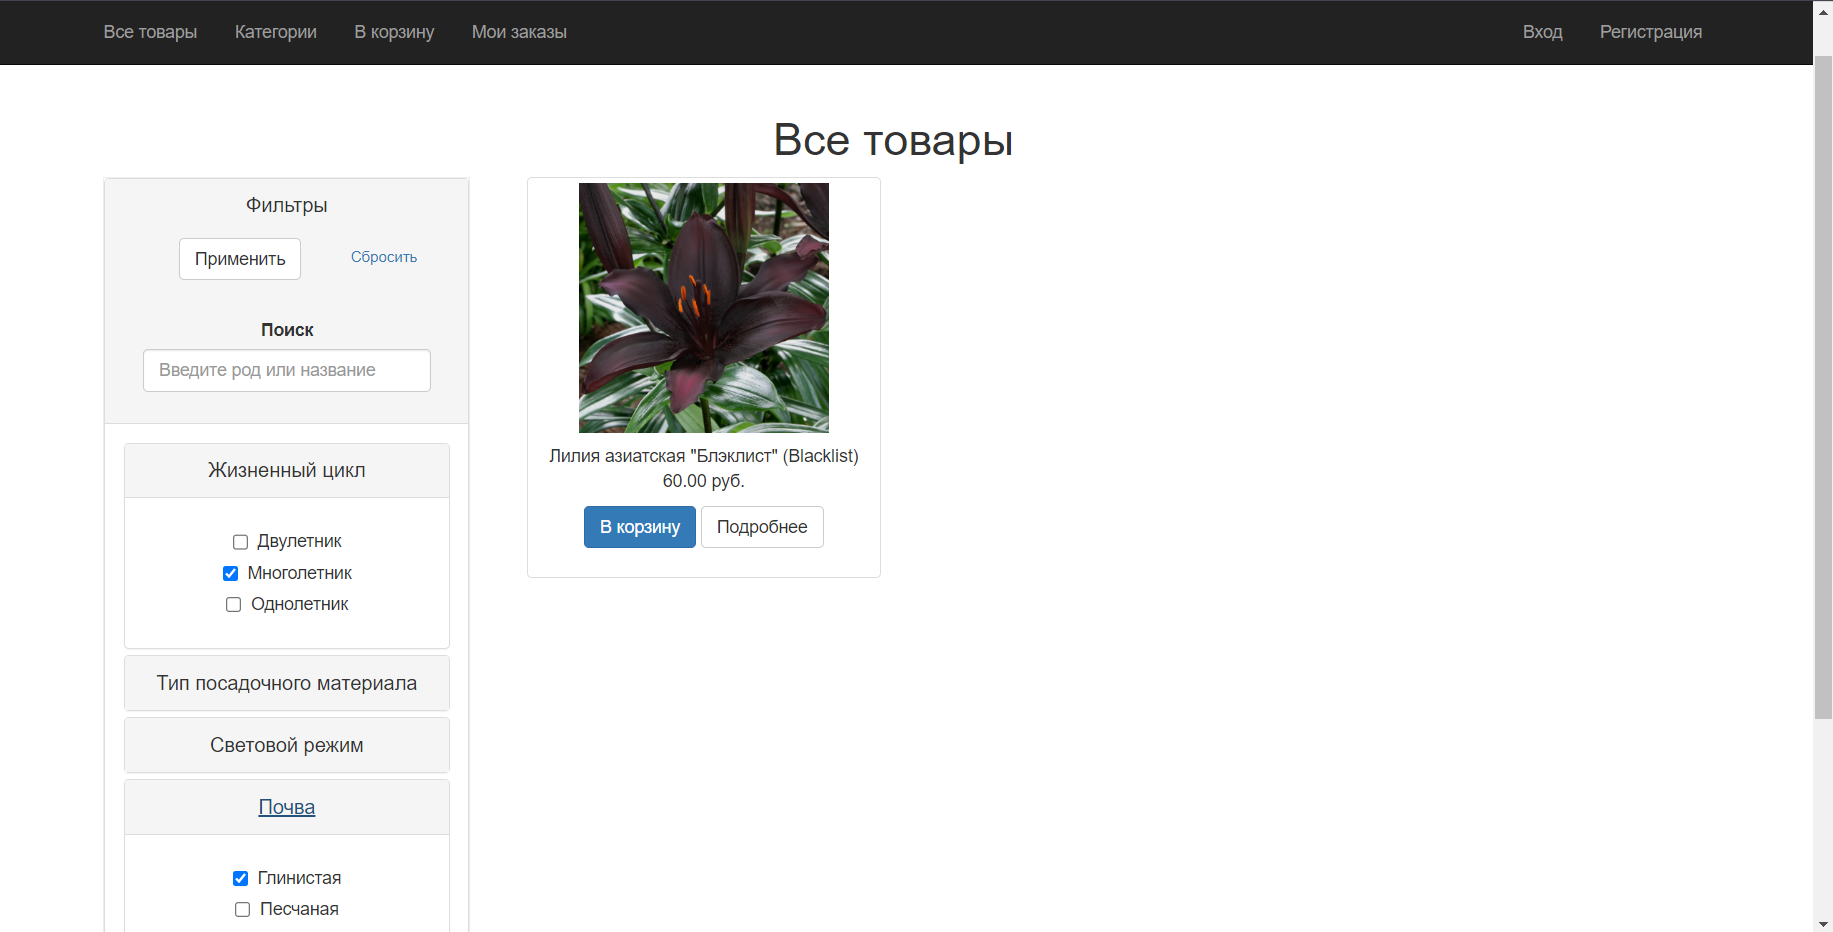
\includegraphics[width=1\linewidth]{2filter}
	\caption{Фильтрация по нескольким параметрам}
	\label{2filter:image}
\end{figure}
%\vspace{-\figureaboveskip} % двойной отступ не нужен (можно использовать, если раздел заканчивается картинкой)

На рисунке \ref{search:image} показан результат поиска товаров по названию.

\begin{figure}[H]
	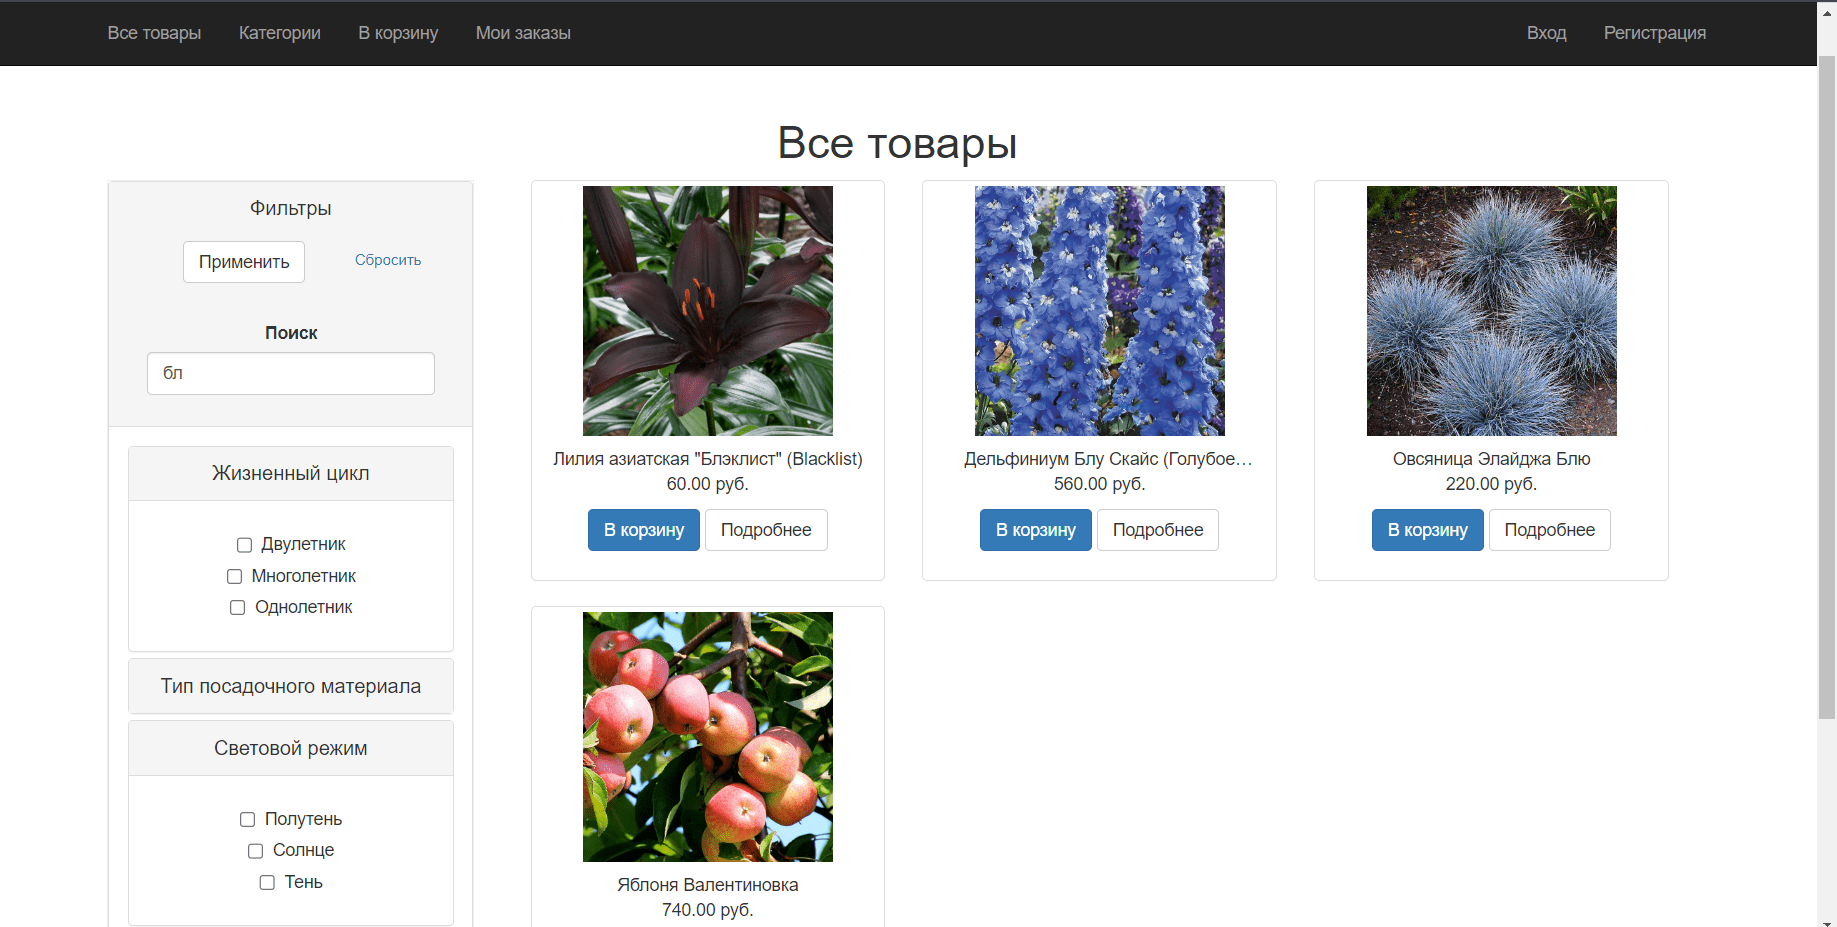
\includegraphics[width=1\linewidth]{search}
	\caption{Поиск по названию}
	\label{search:image}
\end{figure}
%\vspace{-\figureaboveskip} % двойной отступ не нужен (можно использовать, если раздел заканчивается картинкой)

На рисунке \ref{product:image} показана страница одного из товаров.

\begin{figure}[H]
	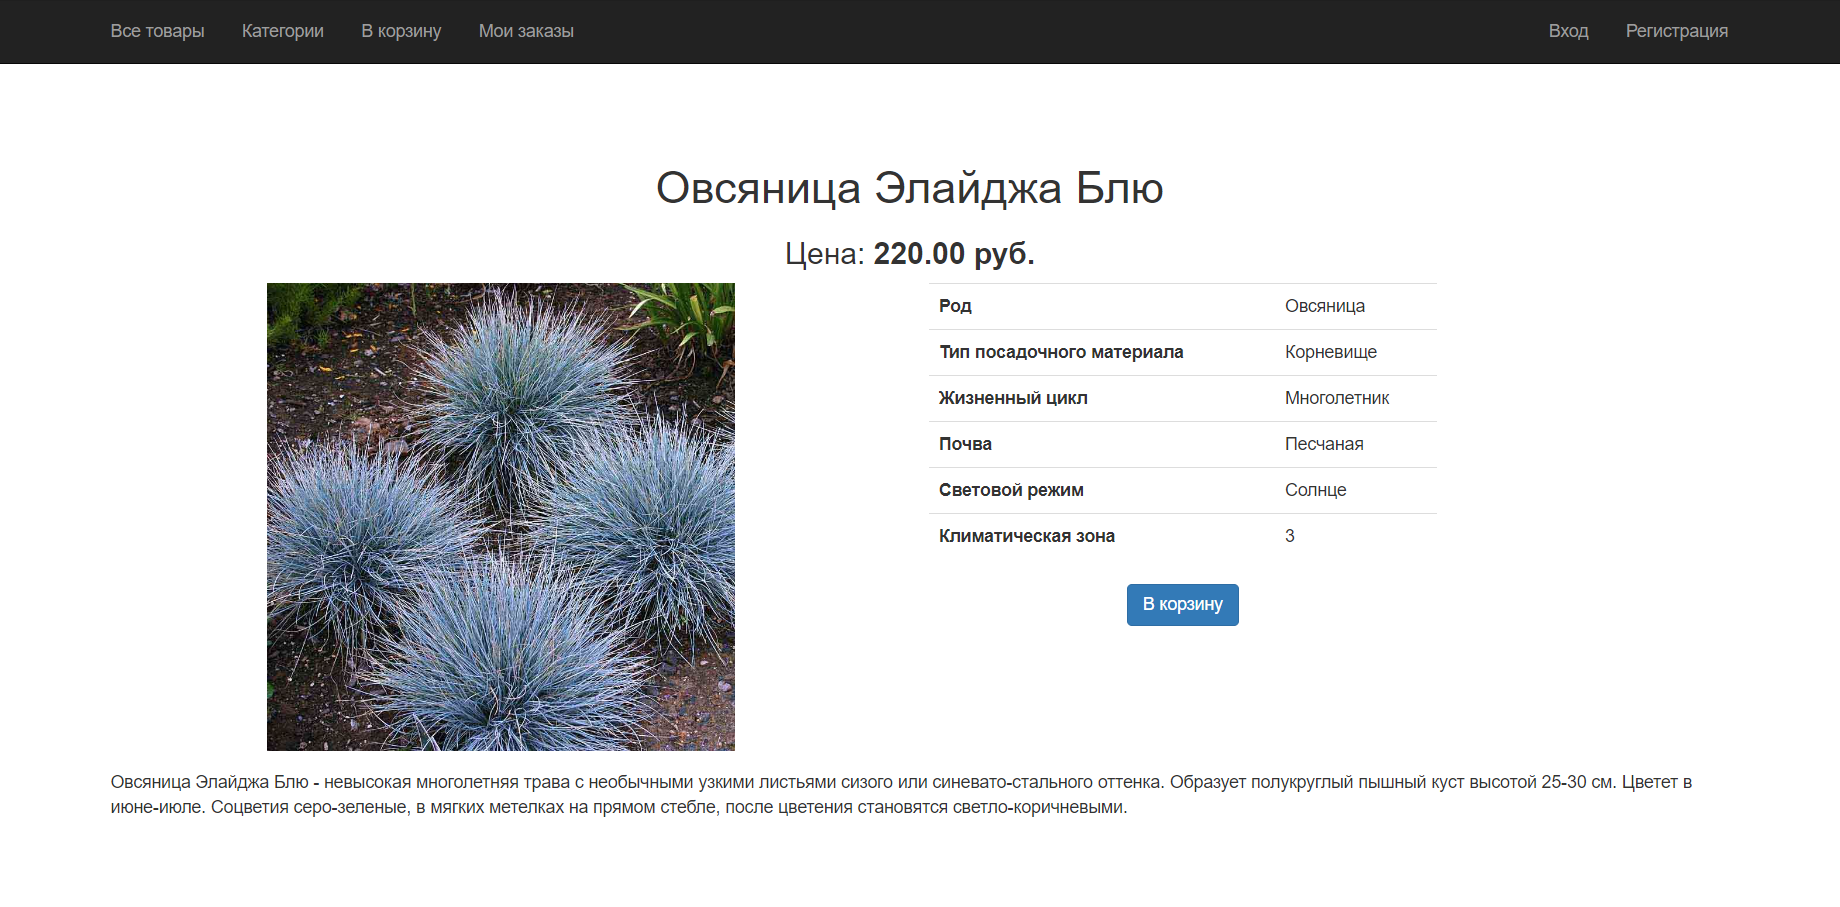
\includegraphics[width=1\linewidth]{product}
	\caption{Страница товара}
	\label{product:image}
\end{figure}
%\vspace{-\figureaboveskip} % двойной отступ не нужен (можно использовать, если раздел заканчивается картинкой)


На рисунке \ref{categories:image} показана страница категорий.

\begin{figure}[H]
	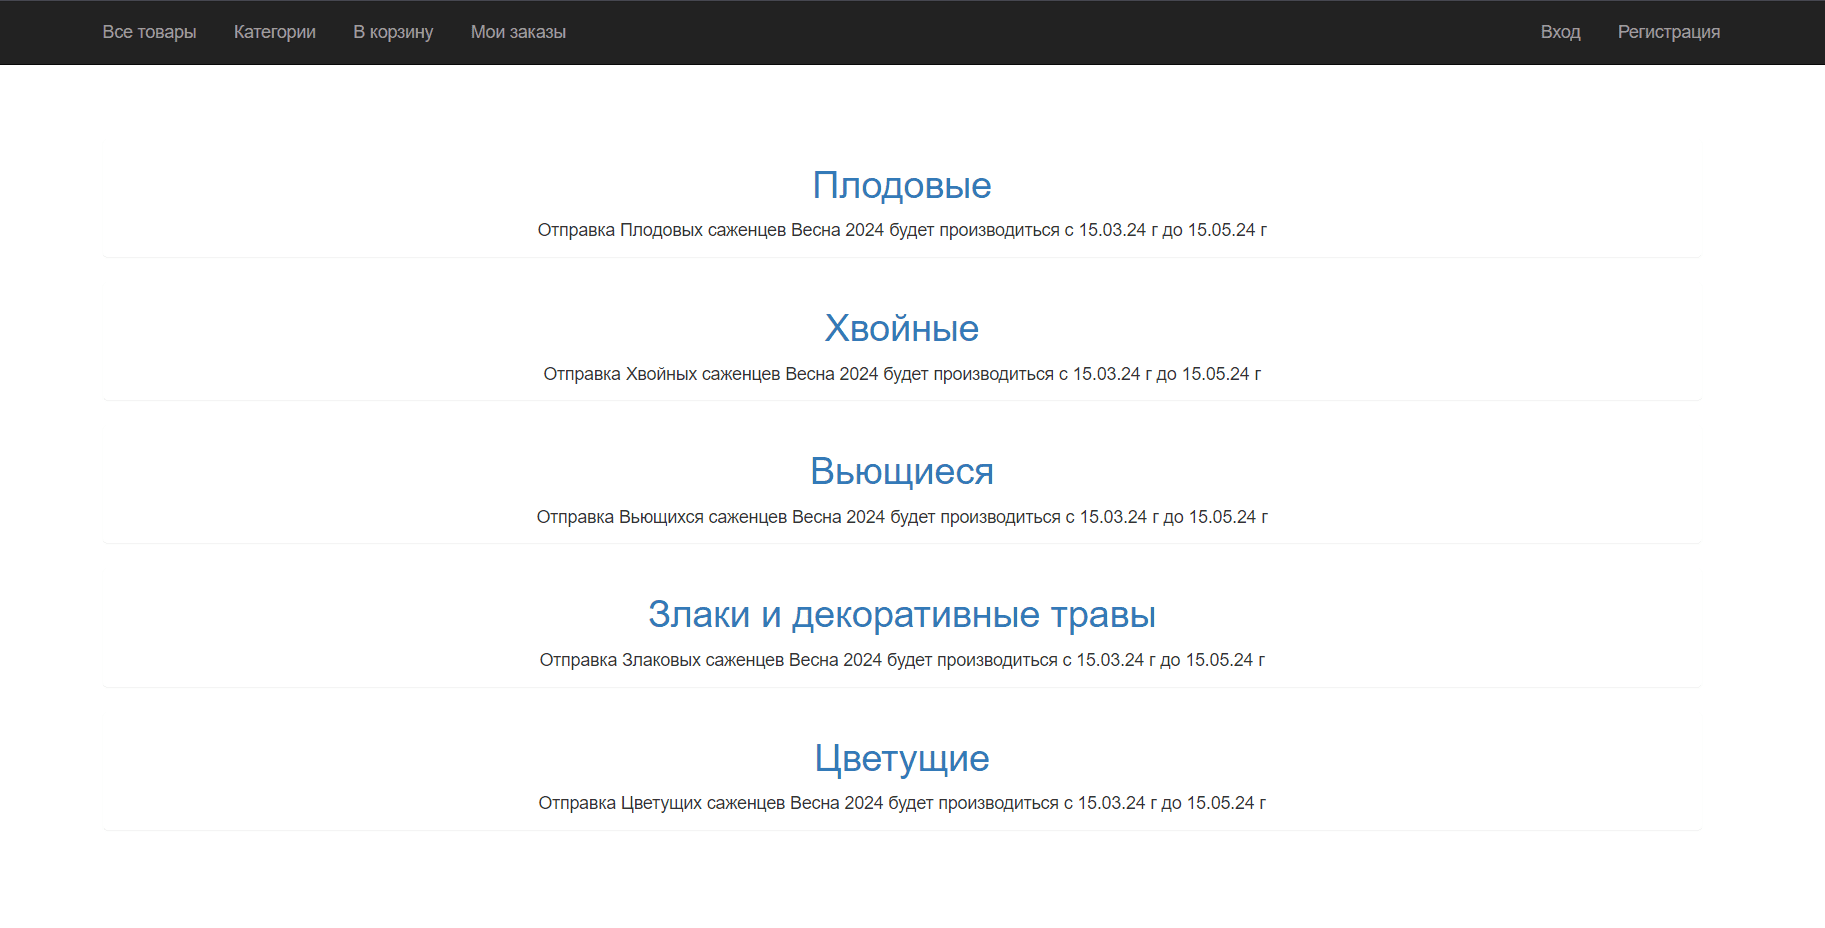
\includegraphics[width=1\linewidth]{categories}
	\caption{Страница категорий}
	\label{categories:image}
\end{figure}
%\vspace{-\figureaboveskip} % двойной отступ не нужен (можно использовать, если раздел заканчивается картинкой)


На рисунке \ref{category:image} показана страница категории <<Злаки и декоративные травы>>.

\begin{figure}[H]
	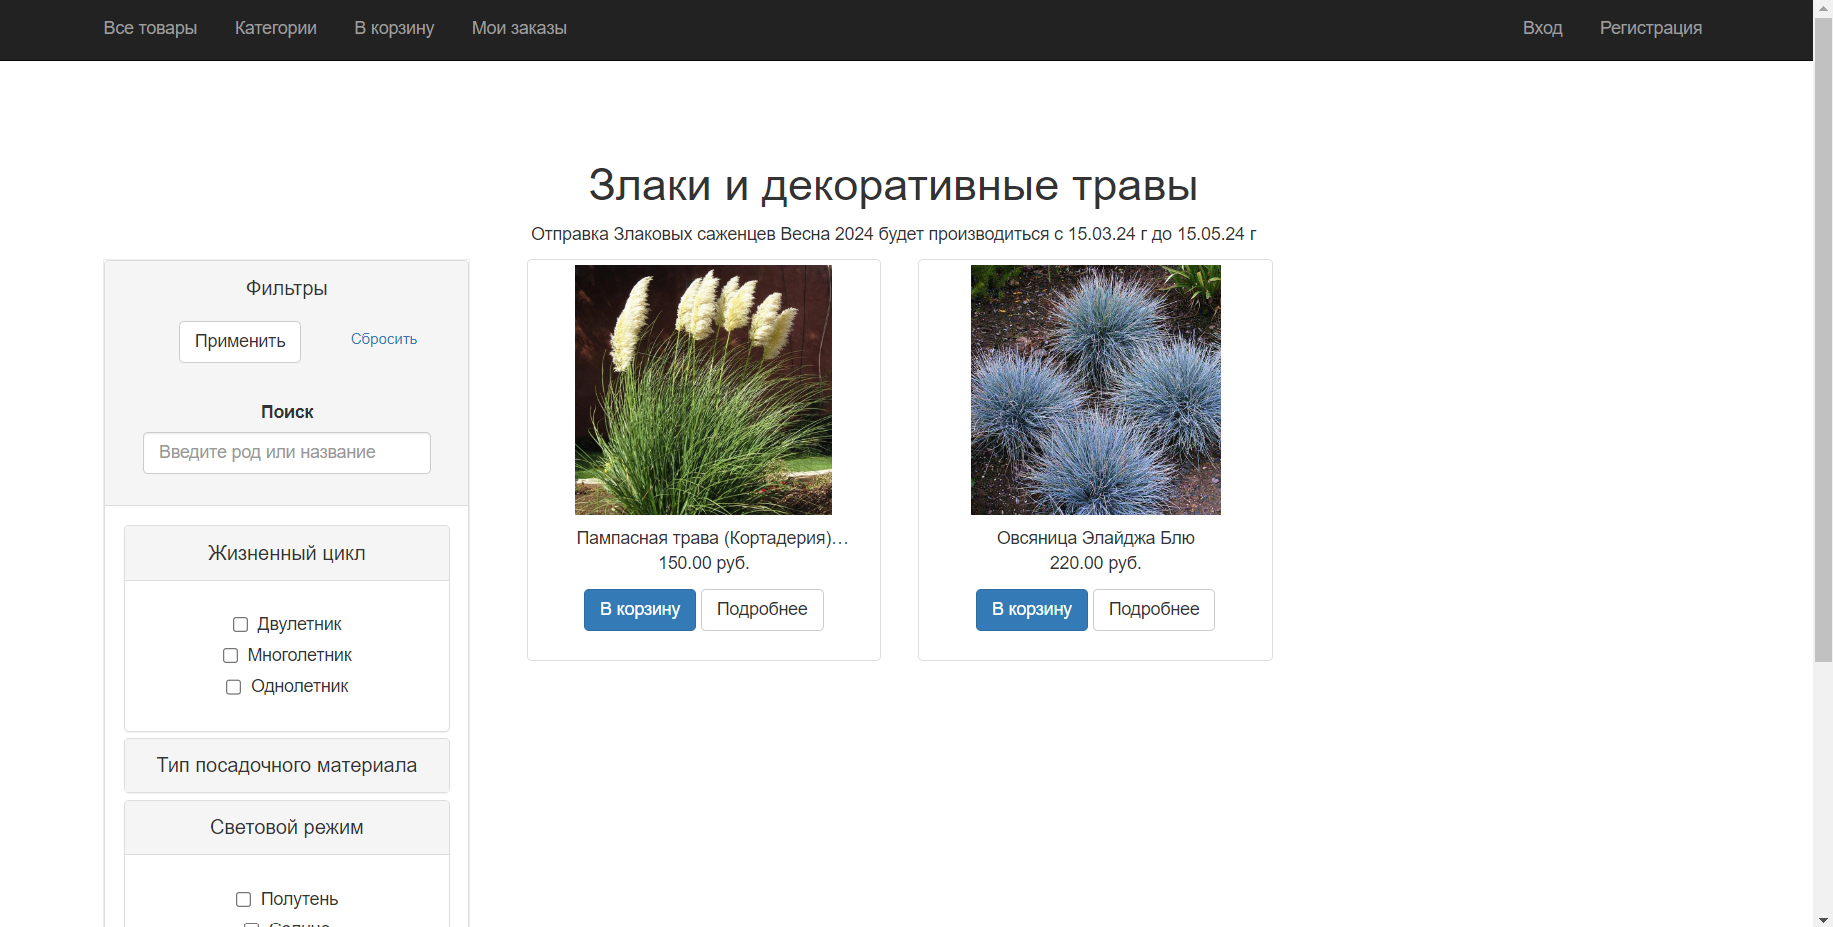
\includegraphics[width=1\linewidth]{category}
	\caption{Страница категории}
	\label{category:image}
\end{figure}
%\vspace{-\figureaboveskip} % двойной отступ не нужен (можно использовать, если раздел заканчивается картинкой)

После применения фильтрации на странице категории выведутся товары, принадлежащие этой категории и соответствующие выбранным значениям характеристик. Это показано на рисунке \ref{categoryFilter:image}.

\begin{figure}[H]
	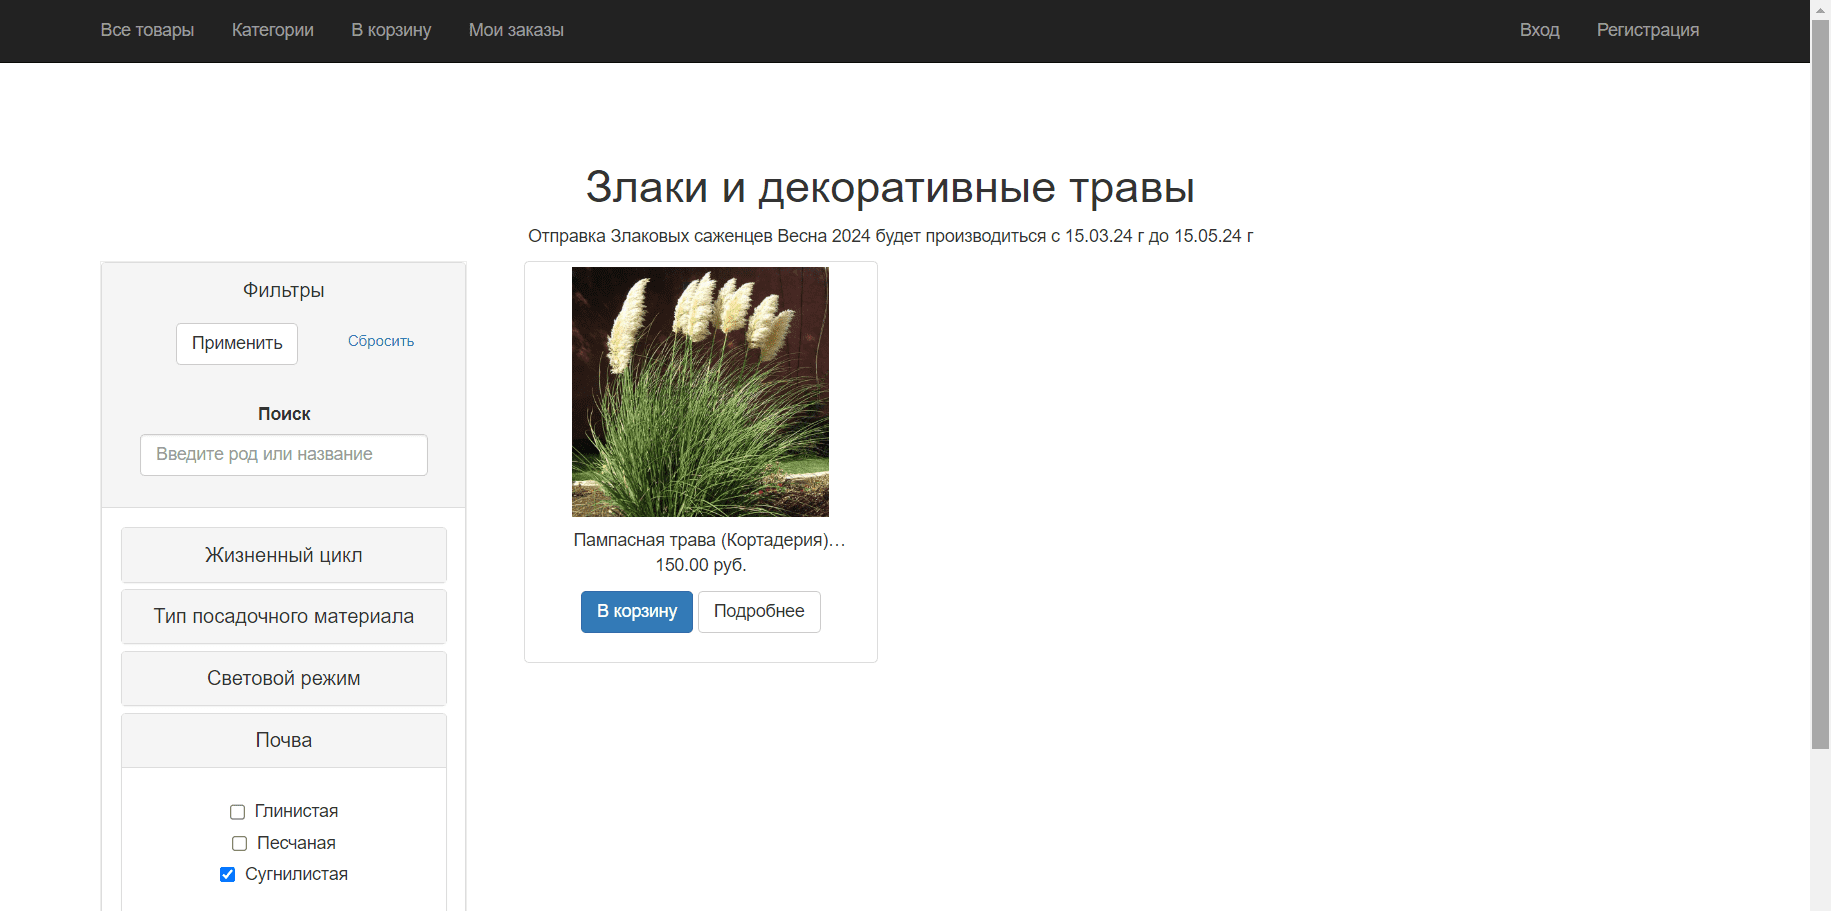
\includegraphics[width=1\linewidth]{categoryFilter}
	\caption{Фильтрация на странице категории}
	\label{categoryFilter:image}
\end{figure}
%\vspace{-\figureaboveskip} % двойной отступ не нужен (можно использовать, если раздел заканчивается картинкой)


На рисунке \ref{basketNull:image} показана корзина до добавления в неё товаров.

\begin{figure}[H]
	
\includegraphics[width=1\linewidth]{basketNull}
	\caption{Пустая корзина}
	\label{basketNull:image}
\end{figure}
%\vspace{-\figureaboveskip} % двойной отступ не нужен (можно использовать, если раздел заканчивается картинкой)

На рисунке \ref{basketAdd:image} показано добавление товара в корзину.

\begin{figure}[H]
	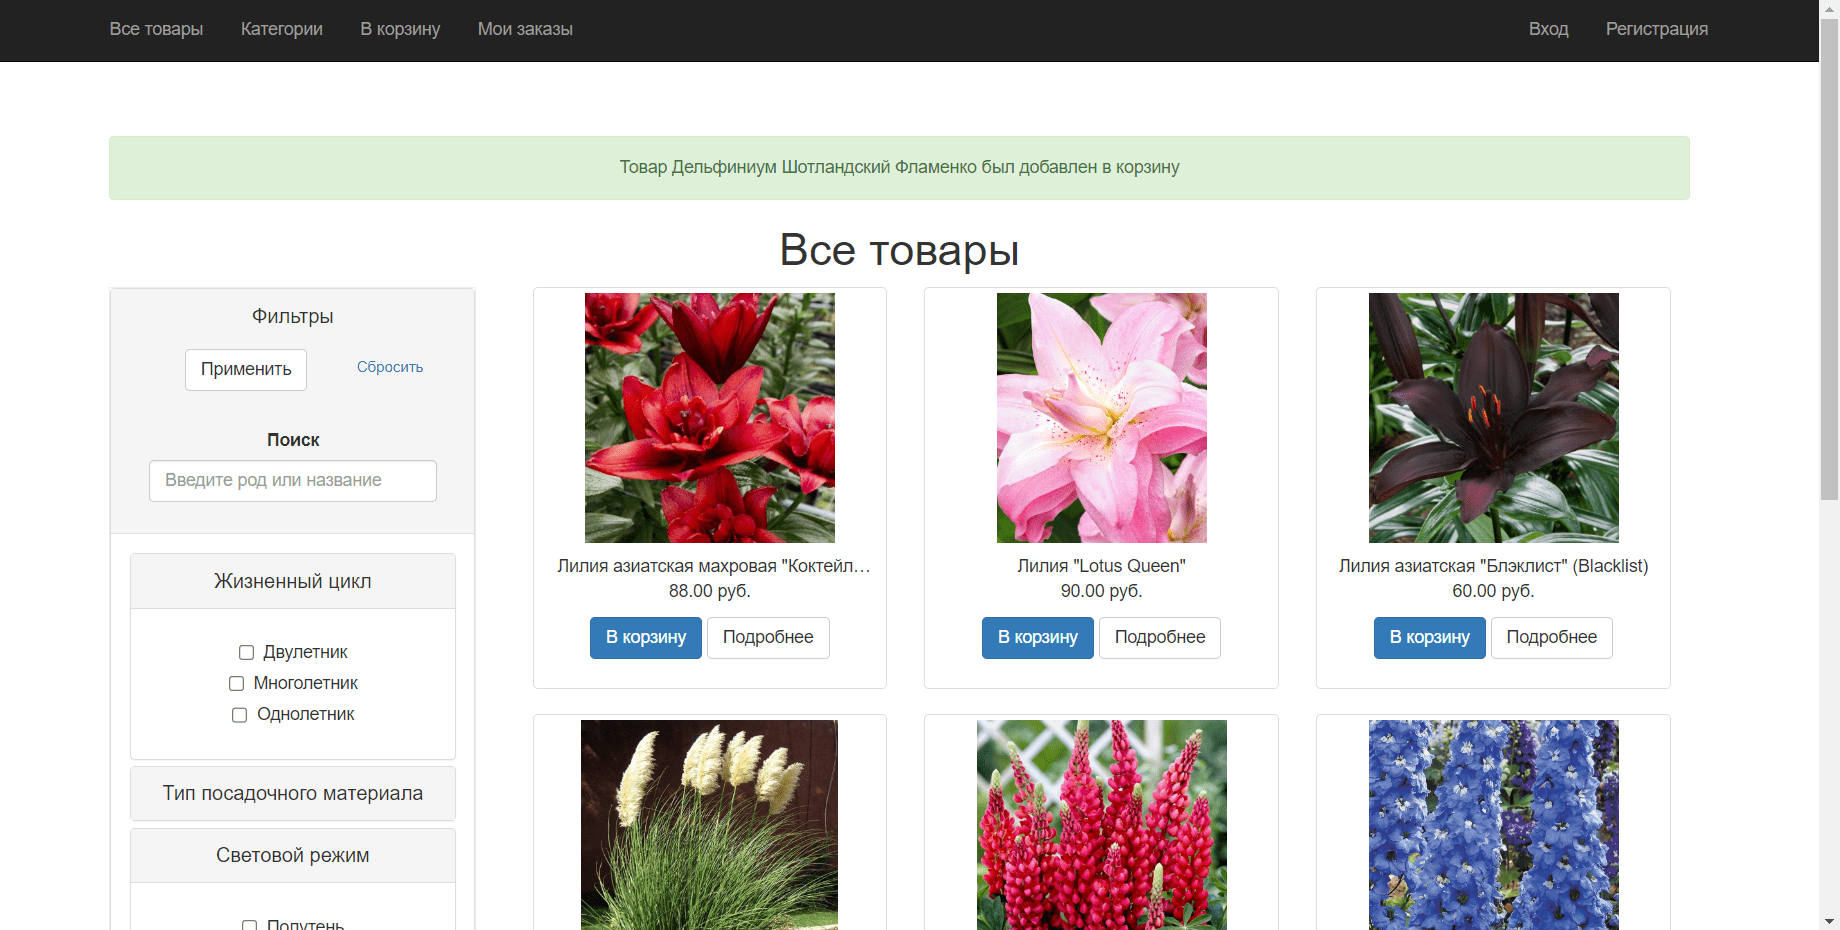
\includegraphics[width=1\linewidth]{basketAdd}
	\caption{Добавление товара в корзину}
	\label{basketAdd:image}
\end{figure}
%\vspace{-\figureaboveskip} % двойной отступ не нужен (можно использовать, если раздел заканчивается картинкой)

На рисунке \ref{basket:image} показана корзина с товарами.

\begin{figure}[H]
	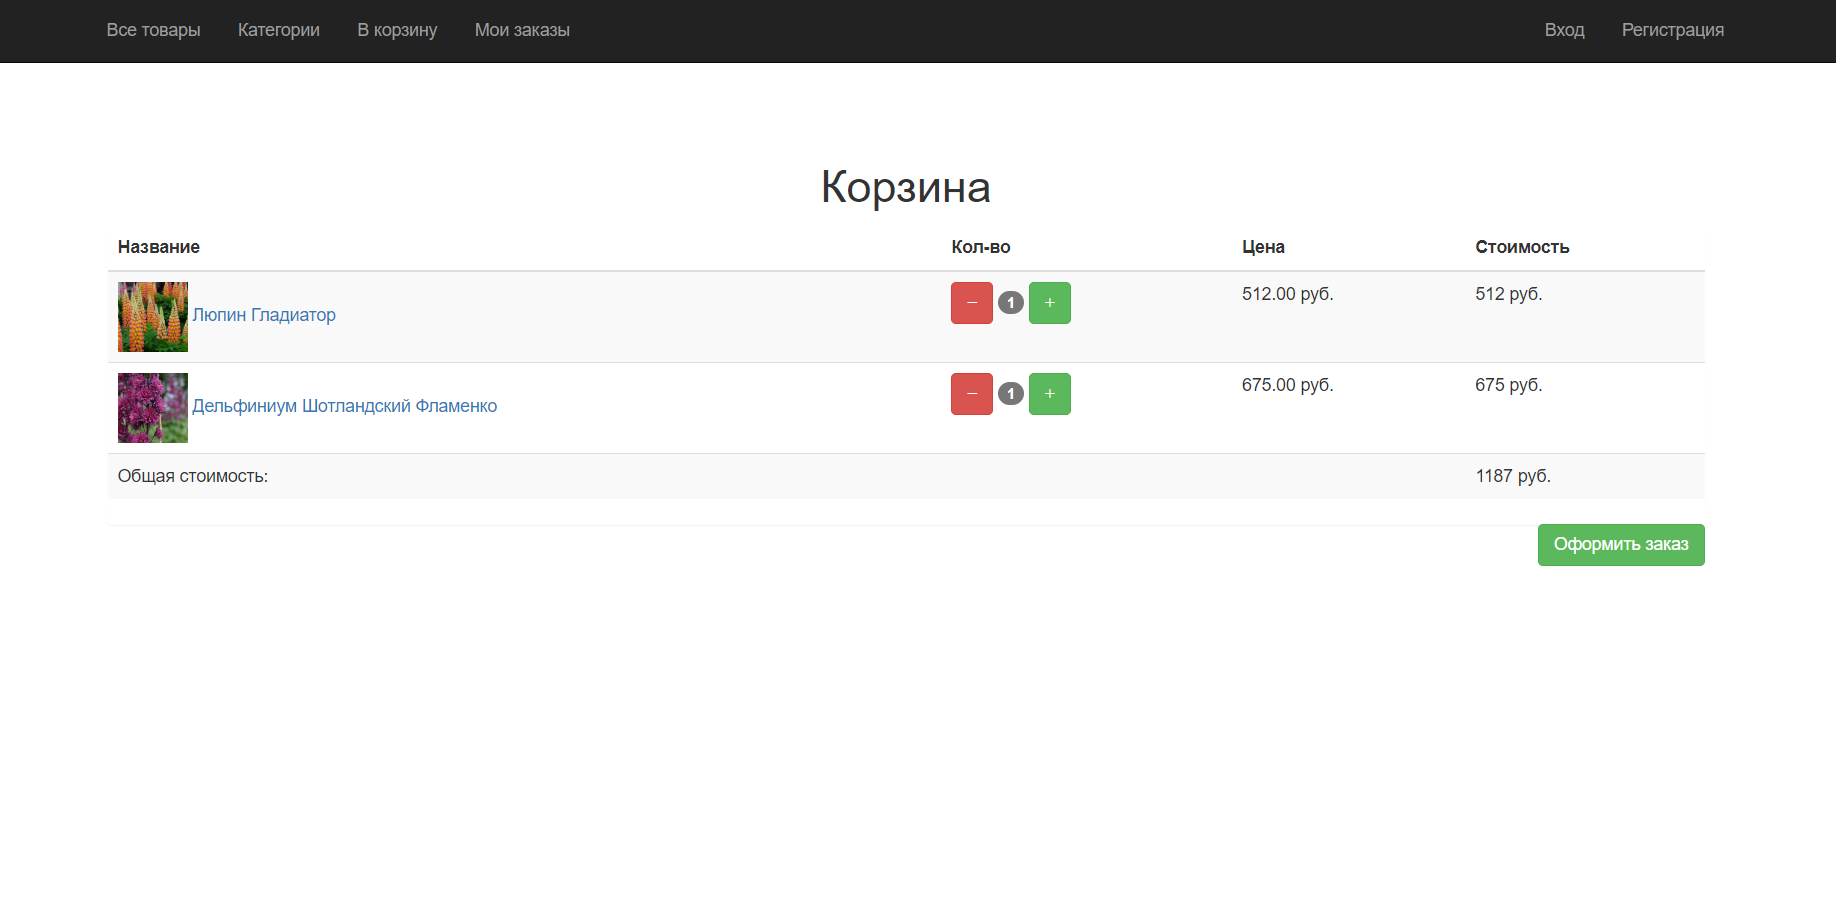
\includegraphics[width=1\linewidth]{basket}
	\caption{Корзина с товарами}
	\label{basket:image}
\end{figure}
%\vspace{-\figureaboveskip} % двойной отступ не нужен (можно использовать, если раздел заканчивается картинкой)

На рисунке \ref{basketRemove:image} показано удаление товара из корзины.

\begin{figure}[H]
	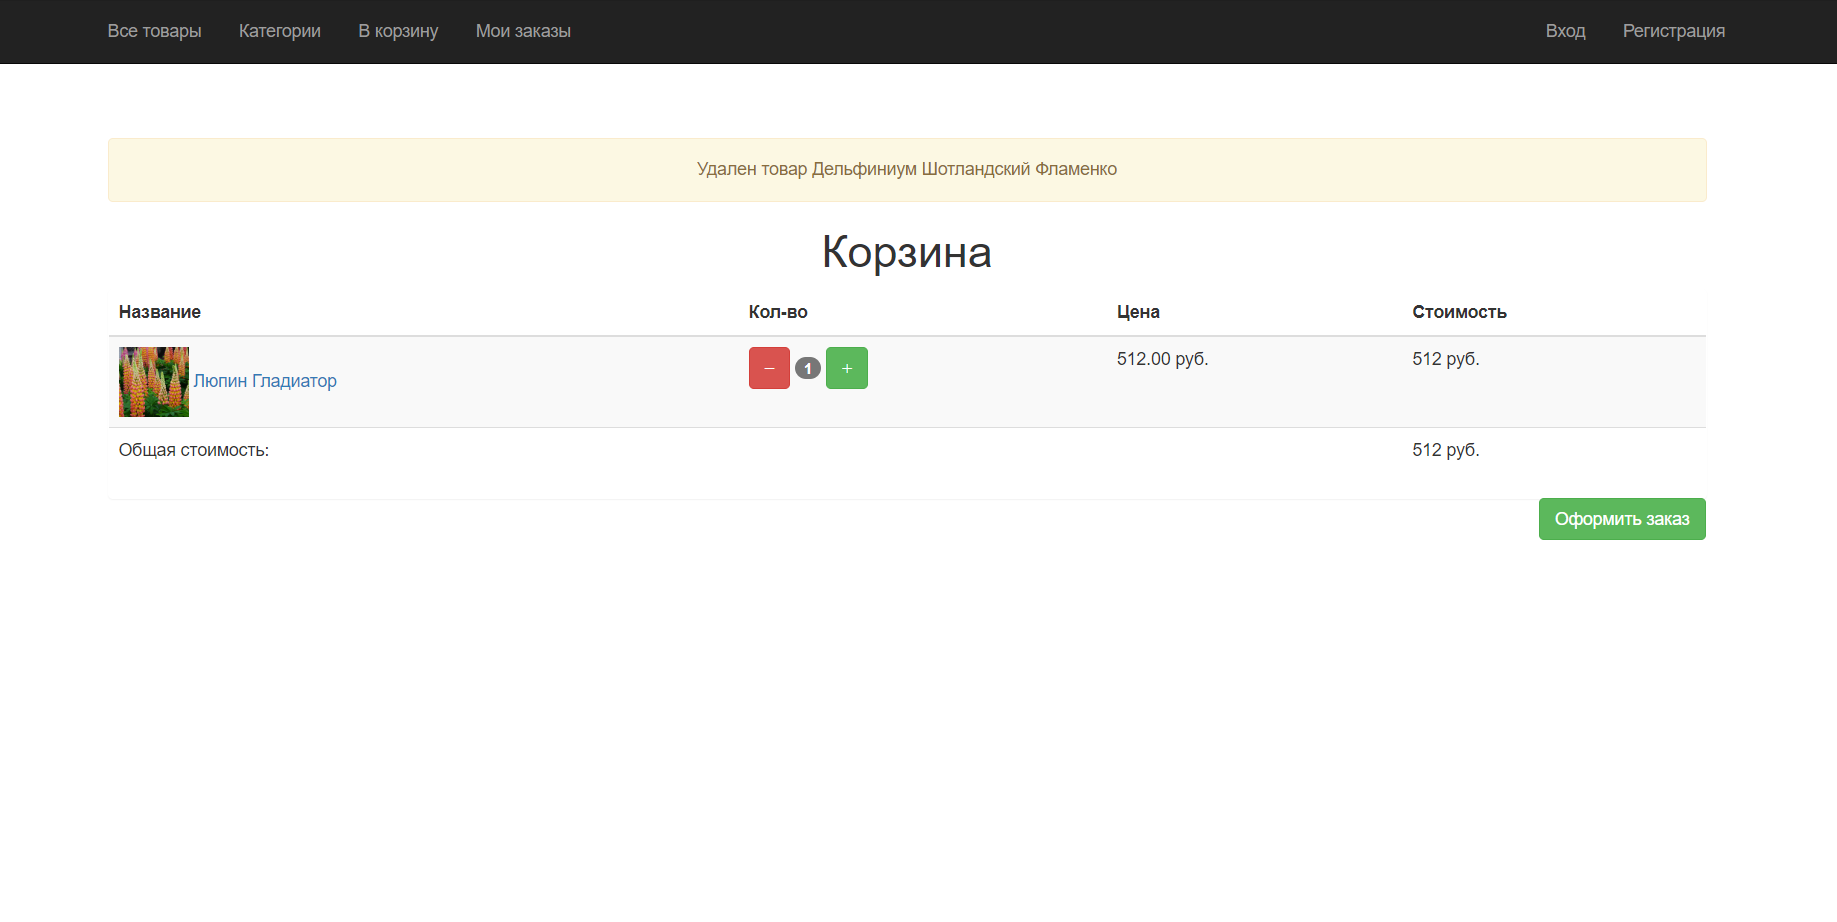
\includegraphics[width=1\linewidth]{basketRemove}
	\caption{Удаление товара из корзины}
	\label{basketRemove:image}
\end{figure}
%\vspace{-\figureaboveskip} % двойной отступ не нужен (можно использовать, если раздел заканчивается картинкой)

На рисунке \ref{confirm:image} показана страница оформления заказа.

\begin{figure}[H]
	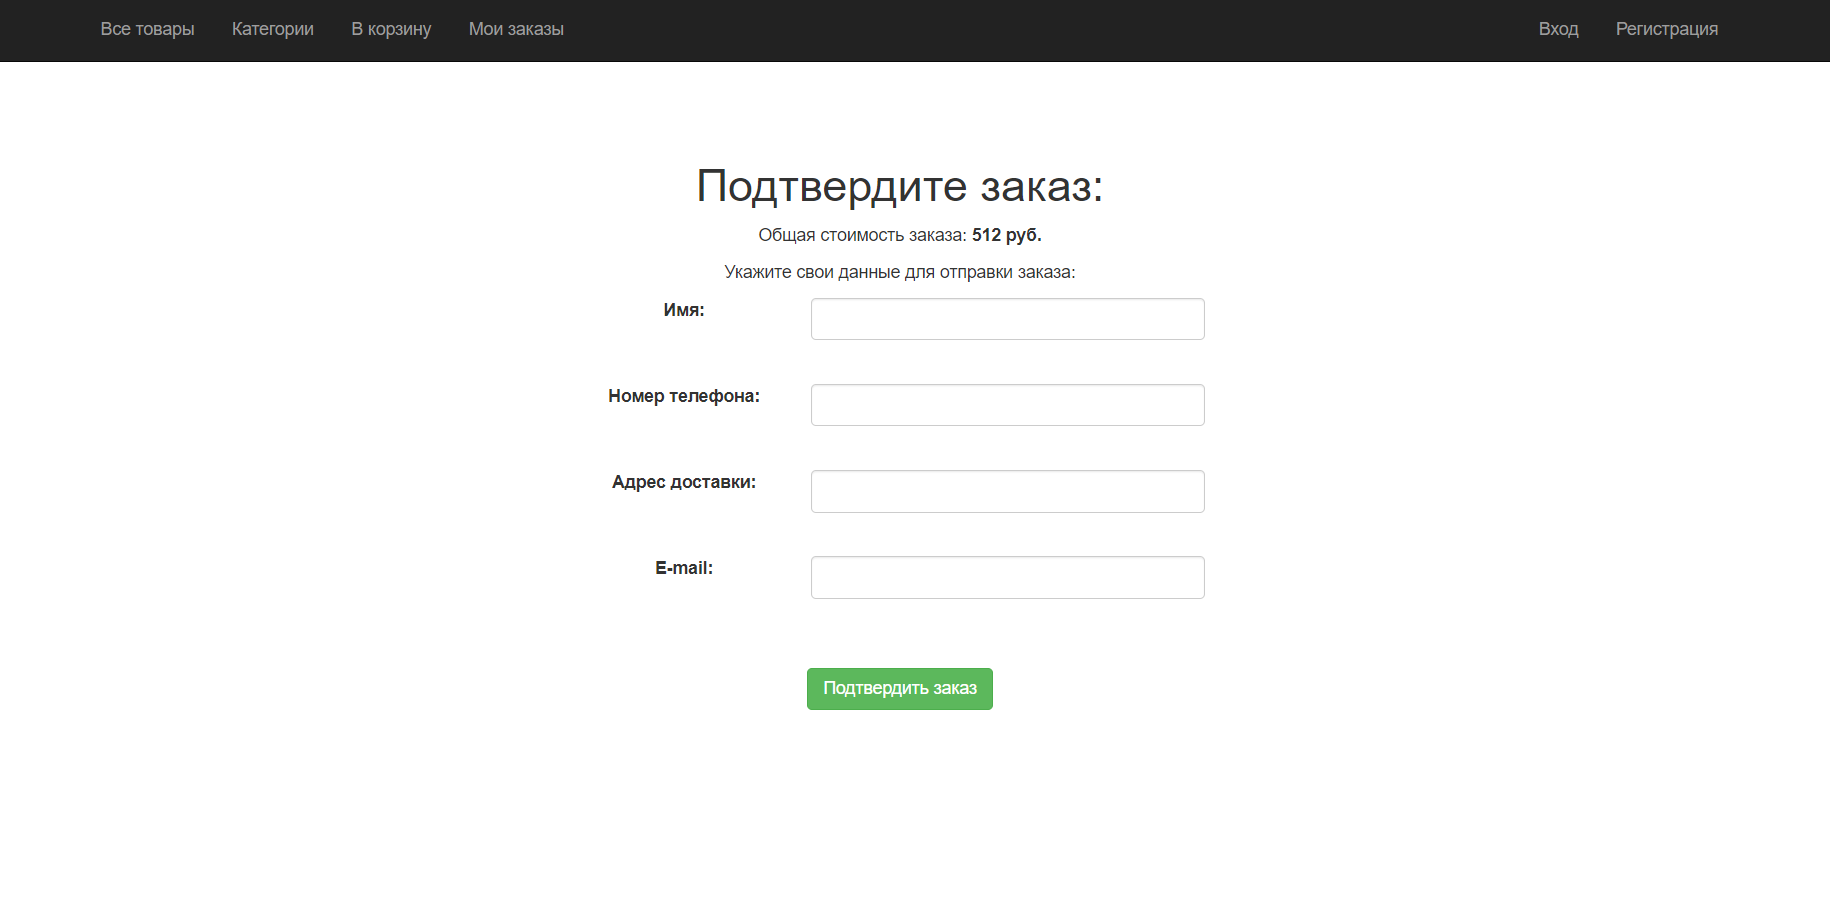
\includegraphics[width=1\linewidth]{confirm}
	\caption{Страница оформления заказа}
	\label{confirm:image}
\end{figure}
%\vspace{-\figureaboveskip} % двойной отступ не нужен (можно использовать, если раздел заканчивается картинкой)

На рисунке \ref{login:image} показана страница входа.

\begin{figure}[H]
	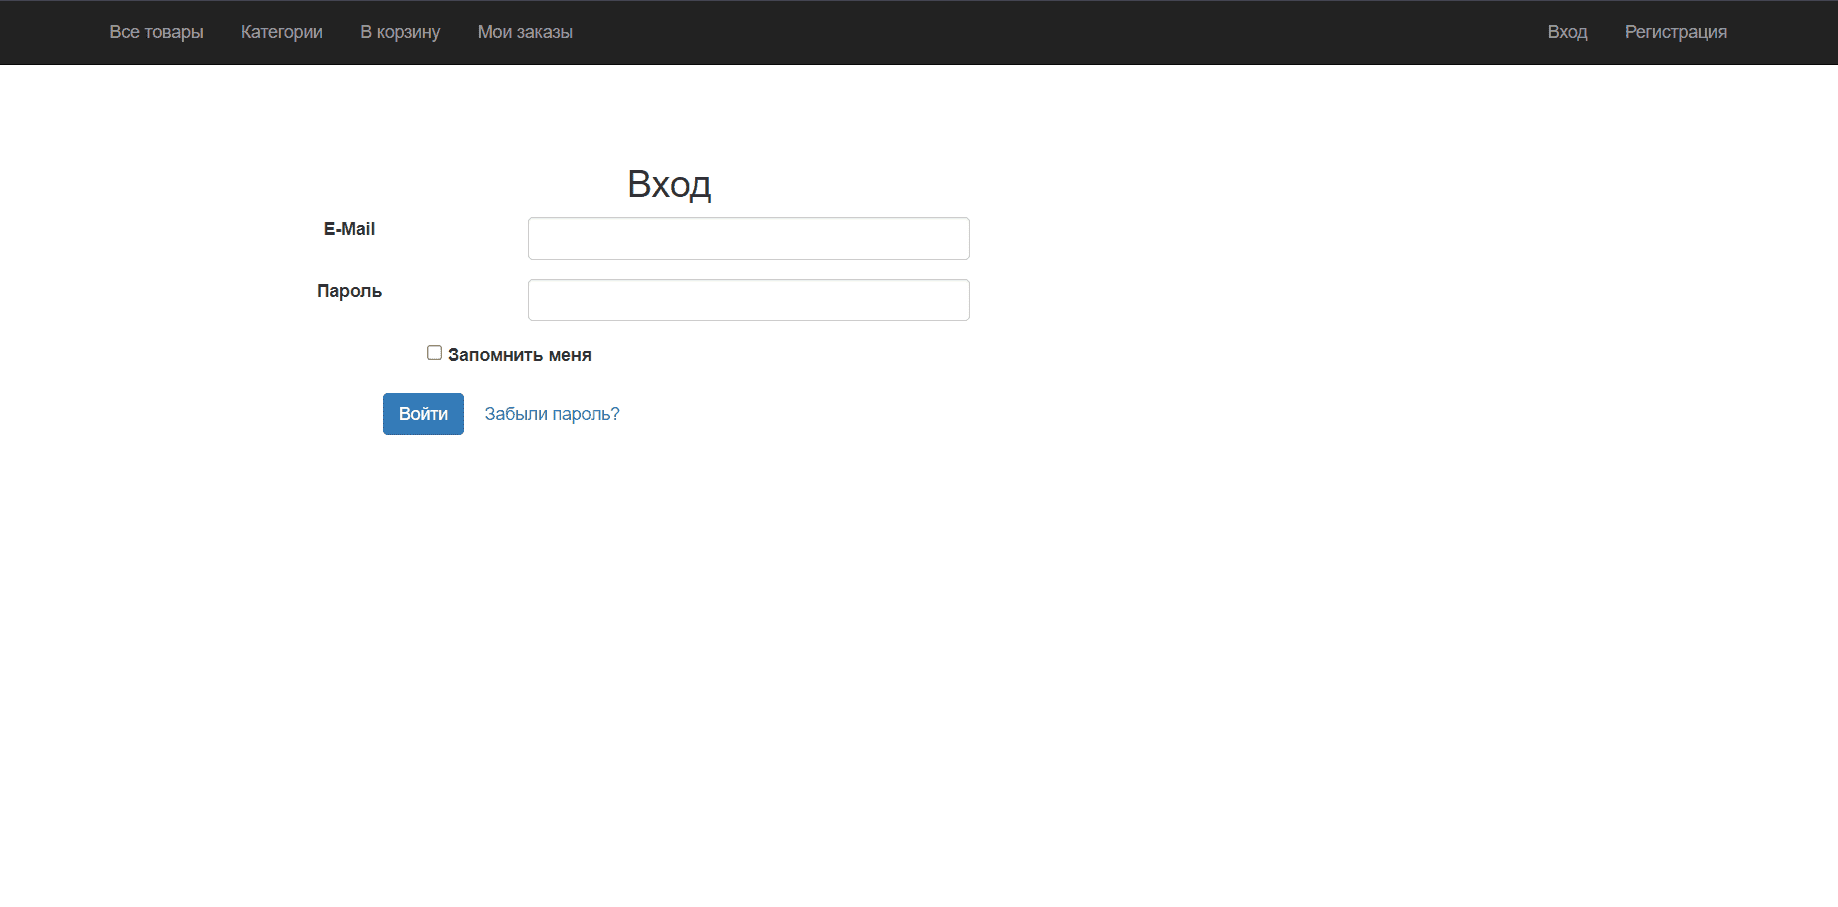
\includegraphics[width=1\linewidth]{login}
	\caption{Страница входа}
	\label{login:image}
\end{figure}
%\vspace{-\figureaboveskip} % двойной отступ не нужен (можно использовать, если раздел заканчивается картинкой)

На рисунке \ref{register:image} показана страница регистрации.

\begin{figure}[H]
	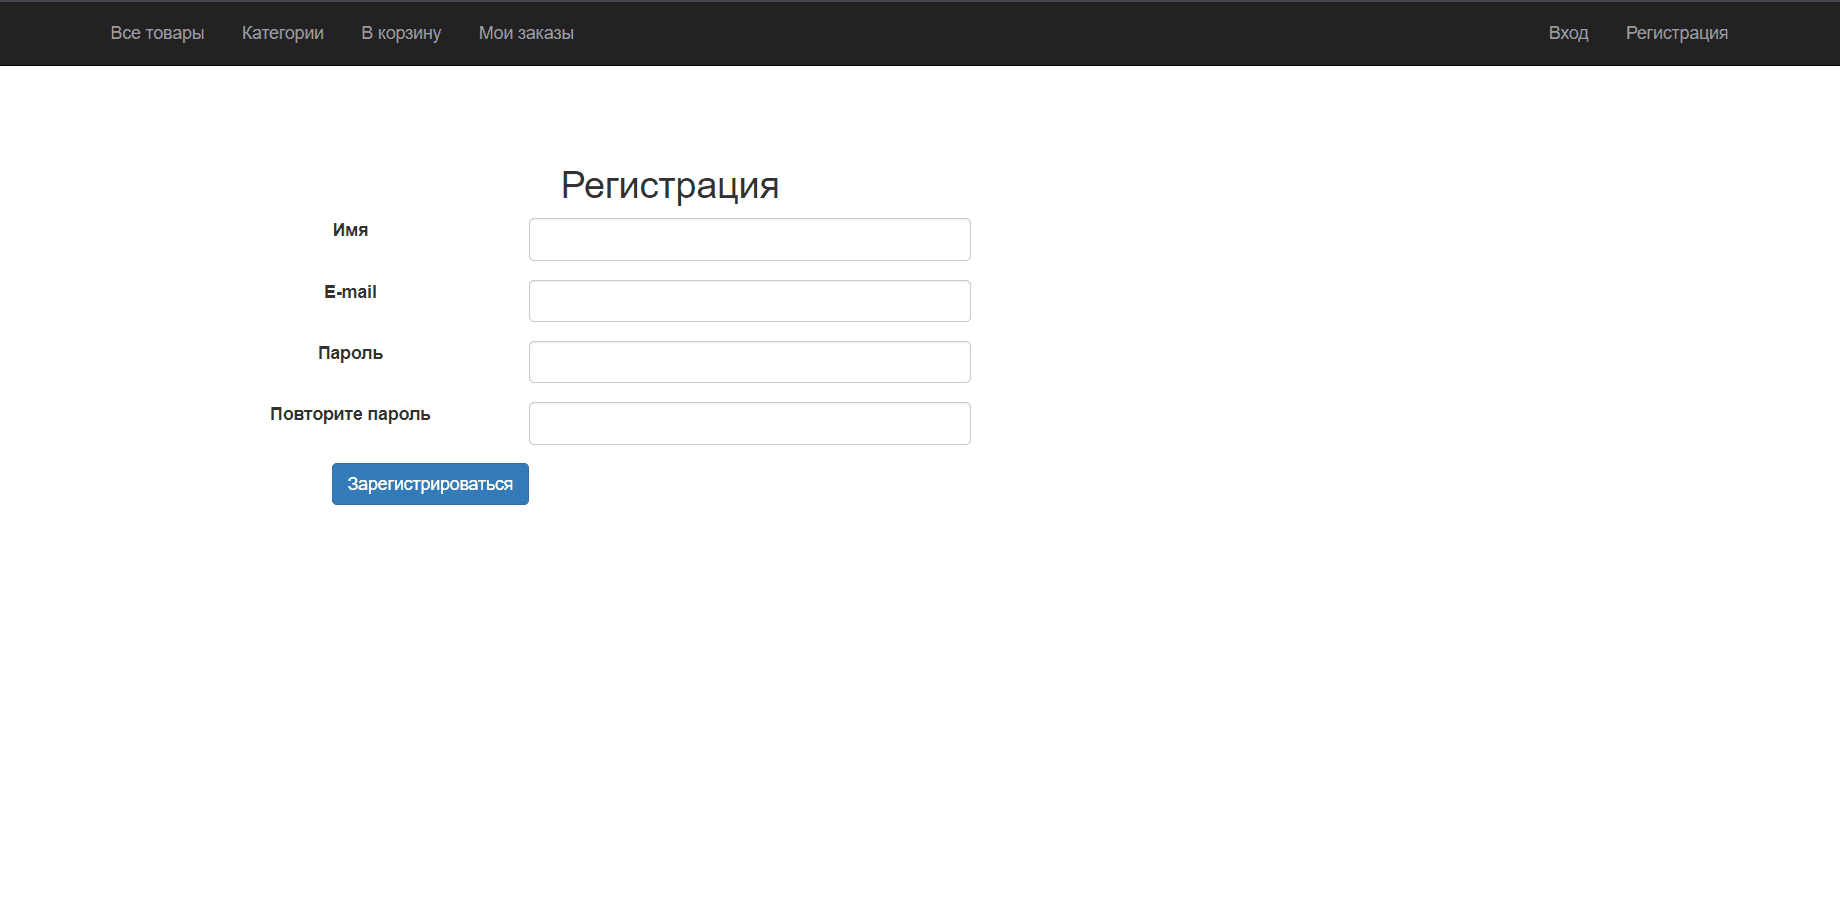
\includegraphics[width=1\linewidth]{register}
	\caption{Страница регистрации}
	\label{register:image}
\end{figure}
%\vspace{-\figureaboveskip} % двойной отступ не нужен (можно использовать, если раздел заканчивается картинкой)

На рисунке \ref{orderSuccess:image} показан результат оформления заказа.

\begin{figure}[H]
	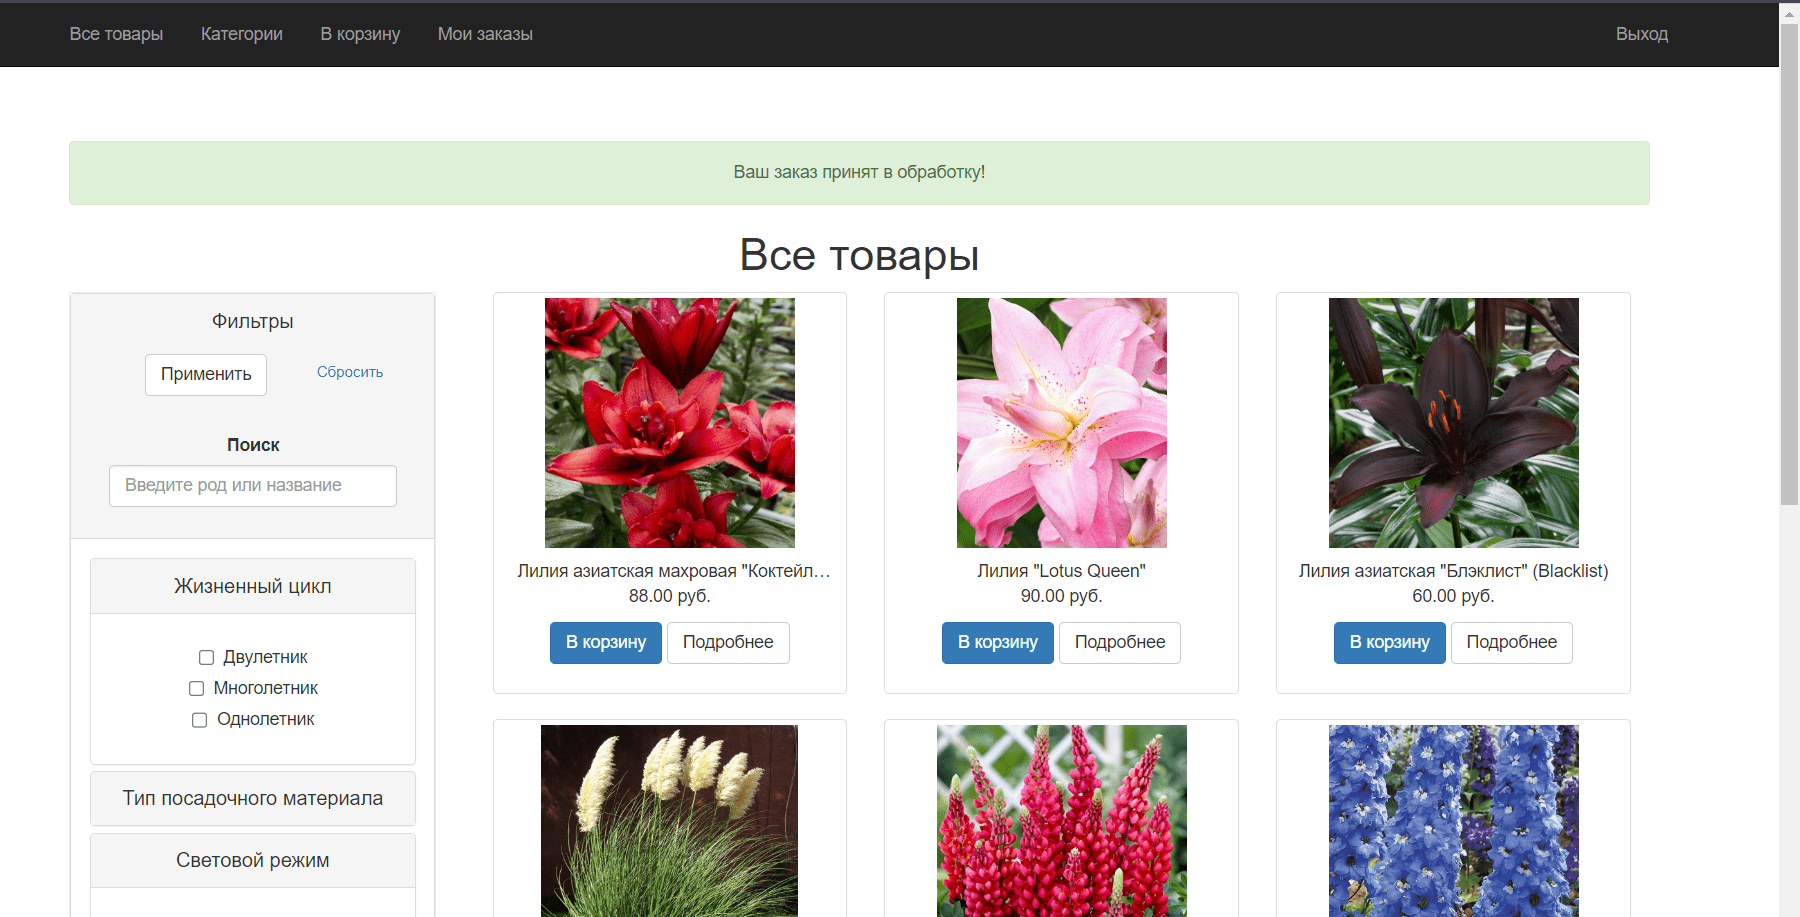
\includegraphics[width=1\linewidth]{orderSuccess}
	\caption{Результат оформления заказа}
	\label{orderSuccess:image}
\end{figure}
%\vspace{-\figureaboveskip} % двойной отступ не нужен (можно использовать, если раздел заканчивается картинкой)

На рисунке \ref{orders:image} показана страница заказов пользователя.

\begin{figure}[H]
	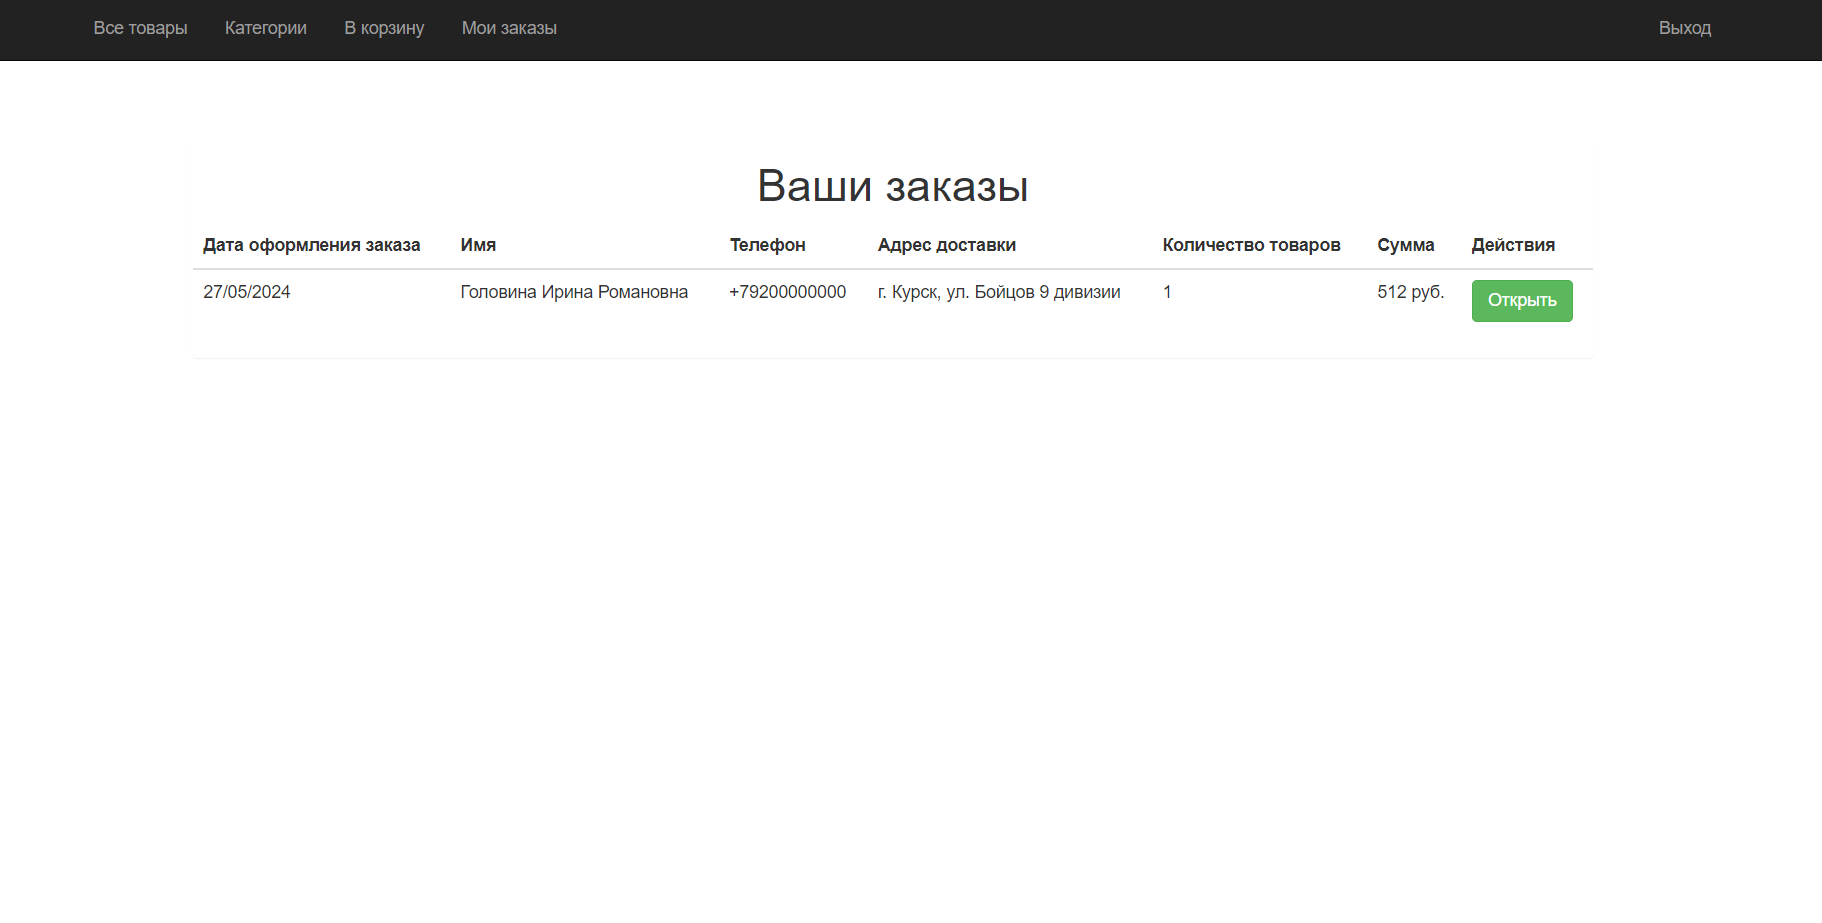
\includegraphics[width=1\linewidth]{orders}
	\caption{Страница заказов пользователя}
	\label{orders:image}
\end{figure}
%\vspace{-\figureaboveskip} % двойной отступ не нужен (можно использовать, если раздел заканчивается картинкой)

На рисунке \ref{order:image} показана страница с деталями заказа пользователя.

\begin{figure}[H]
	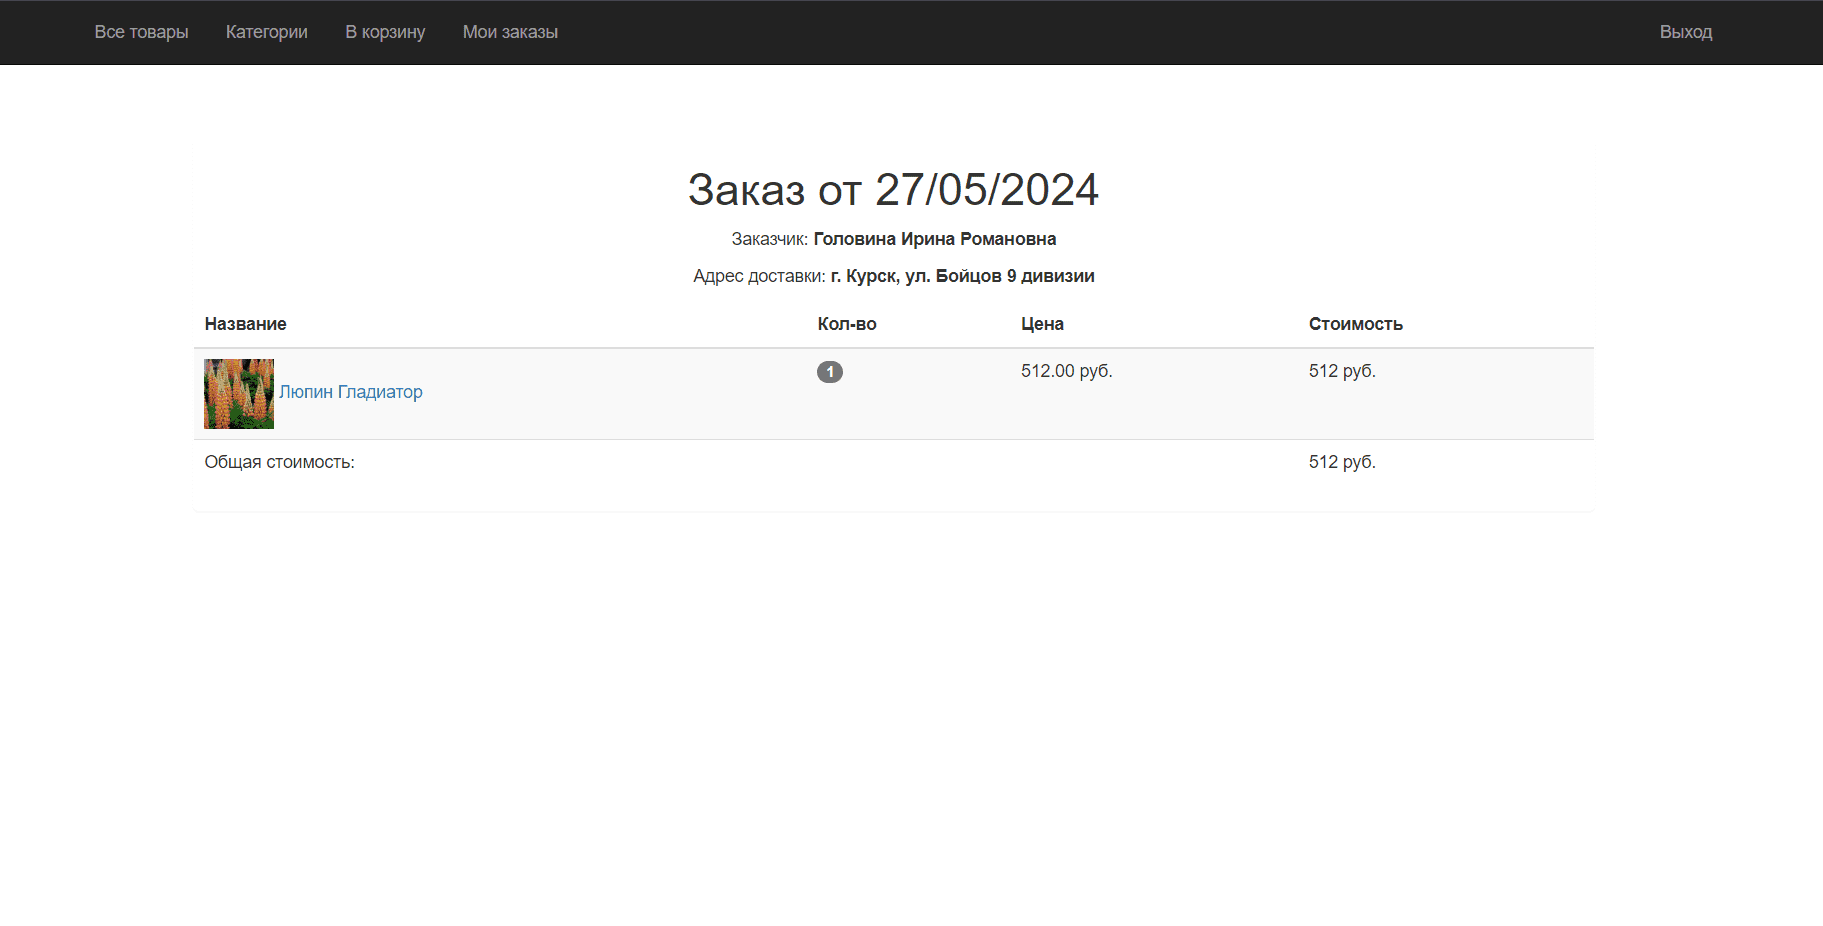
\includegraphics[width=1\linewidth]{order}
	\caption{Страница заказа пользователя}
	\label{order:image}
\end{figure}
%\vspace{-\figureaboveskip} % двойной отступ не нужен (можно использовать, если раздел заканчивается картинкой)




На рисунке \ref{ordersAdmin:image} показана страница заказов в панели администратора.

\begin{figure}[H]
	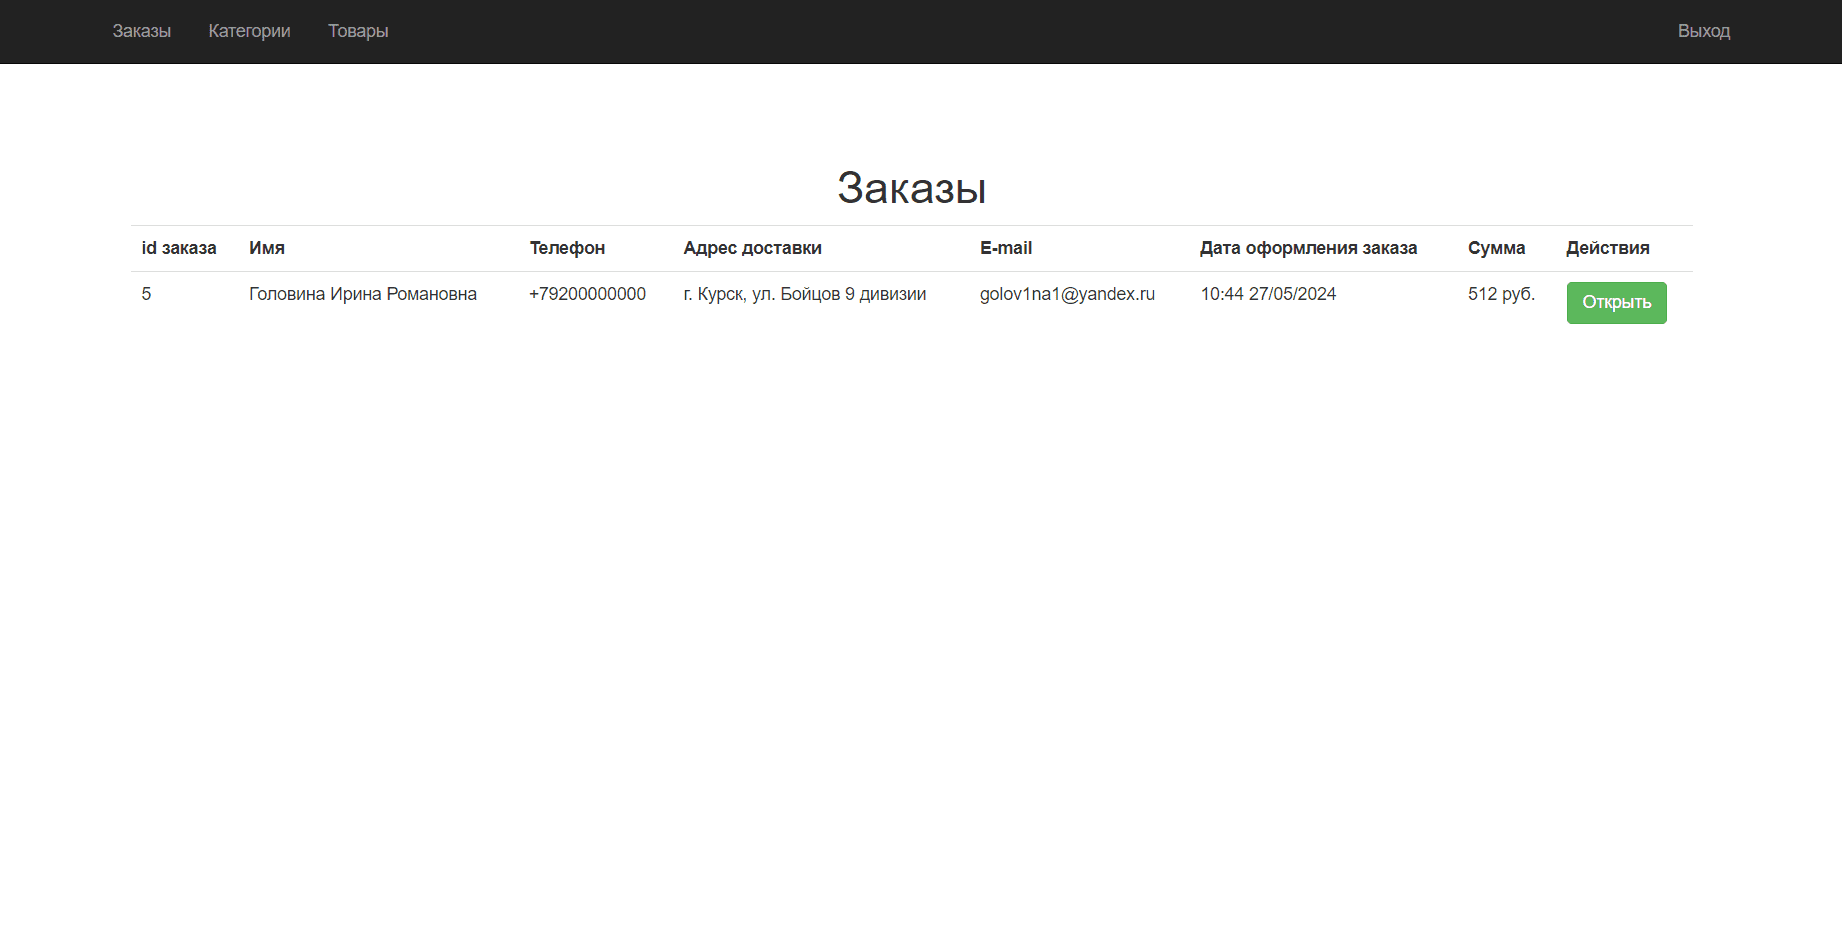
\includegraphics[width=1\linewidth]{ordersAdmin}
	\caption{Страница заказов в панели администратора}
	\label{ordersAdmin:image}
\end{figure}
%\vspace{-\figureaboveskip} % двойной отступ не нужен (можно использовать, если раздел заканчивается картинкой)

На рисунке \ref{orderAdmin:image} показана страница с деталями заказа в панели администратора.

\begin{figure}[H]
	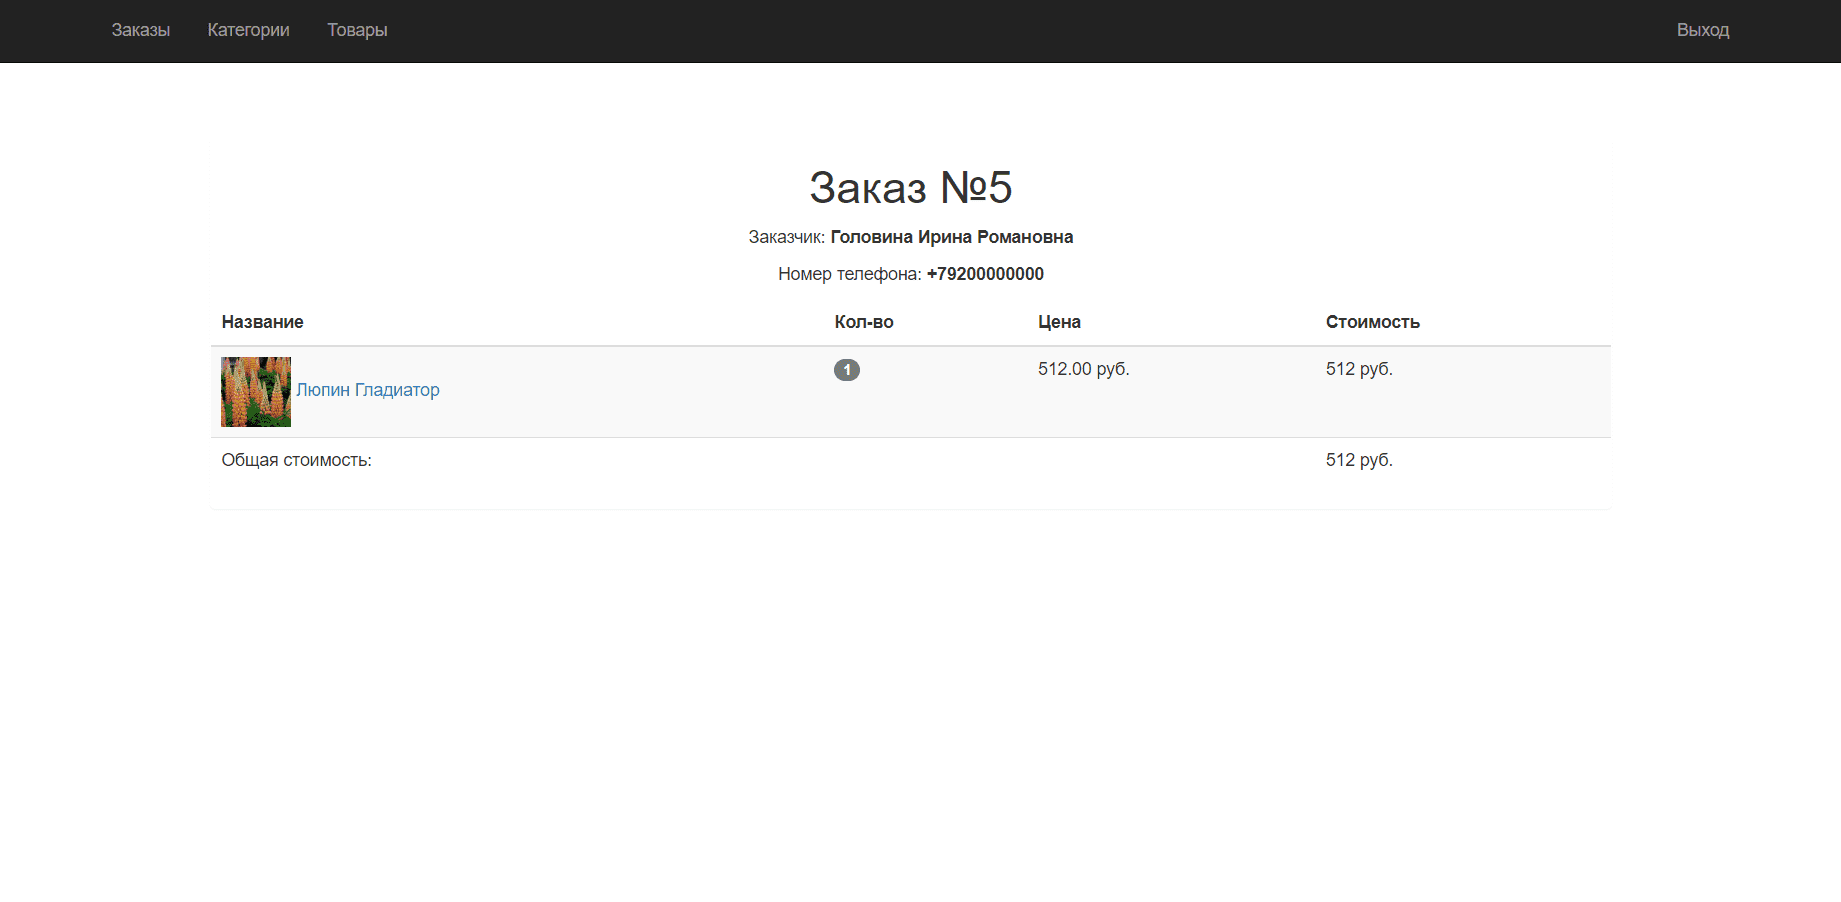
\includegraphics[width=1\linewidth]{orderAdmin}
	\caption{Страница заказа в панели администратора}
	\label{orderAdmin:image}
\end{figure}
%\vspace{-\figureaboveskip} % двойной отступ не нужен (можно использовать, если раздел заканчивается картинкой)

На рисунке \ref{categoriesAdmin:image} показана страница категорий в панели администратора.

\begin{figure}[H]
	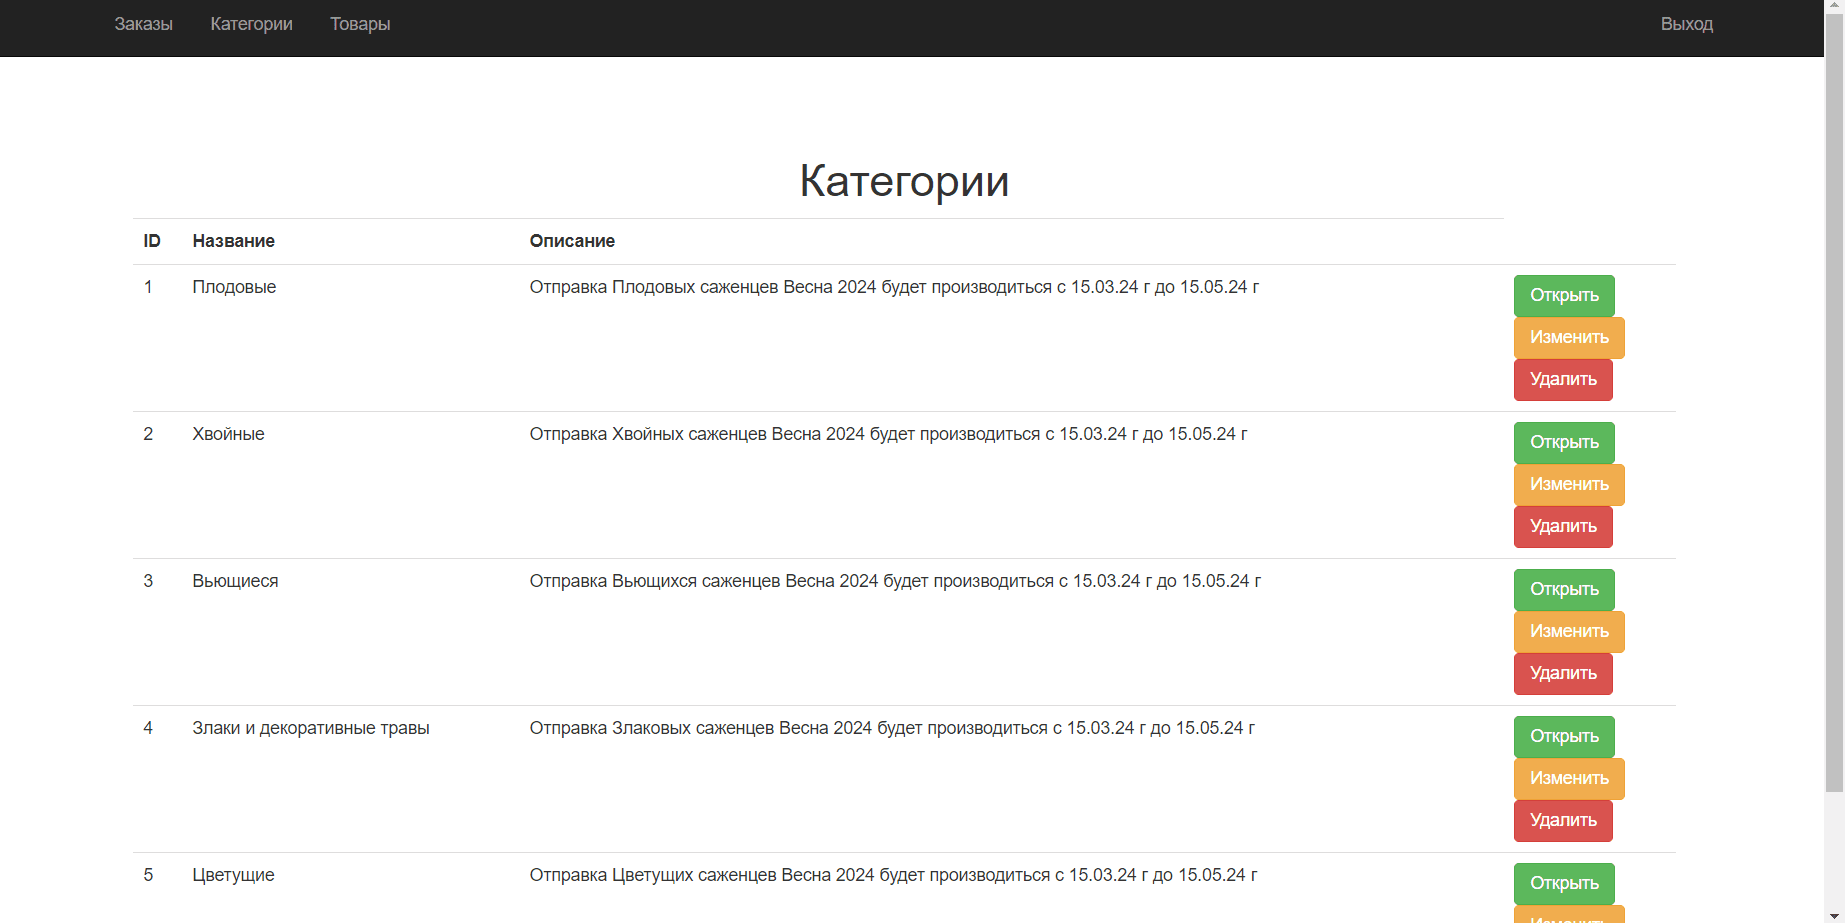
\includegraphics[width=1\linewidth]{categoriesAdmin}
	\caption{Страница категорий в панели администратора}
	\label{categoriesAdmin:image}
\end{figure}
%\vspace{-\figureaboveskip} % двойной отступ не нужен (можно использовать, если раздел заканчивается картинкой)

На рисунке \ref{categoryAdmin:image} показана страница категории <<Плодовые>> в панели администратора.

\begin{figure}[H]
	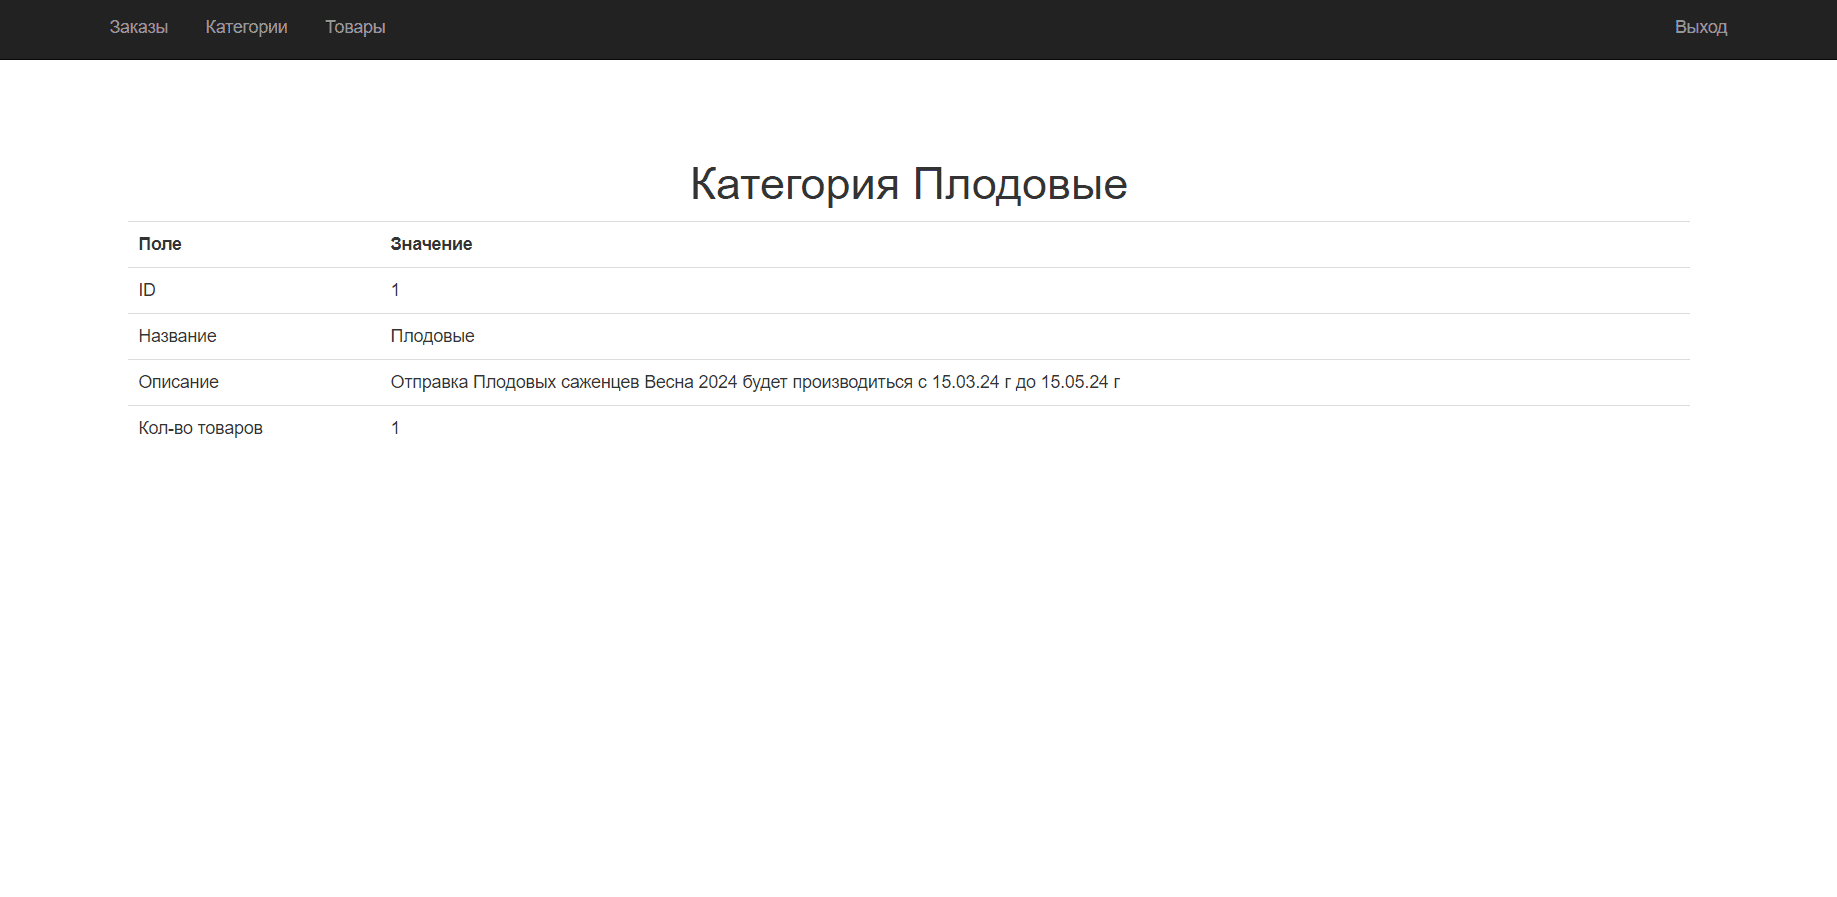
\includegraphics[width=1\linewidth]{categoryAdmin}
	\caption{Страница категории в панели администратора}
	\label{categoryAdmin:image}
\end{figure}
%\vspace{-\figureaboveskip} % двойной отступ не нужен (можно использовать, если раздел заканчивается картинкой)

На рисунке \ref{categoryEdit:image} показана страница редактирования категории <<Плодовые>> в панели администратора.

\begin{figure}[H]
	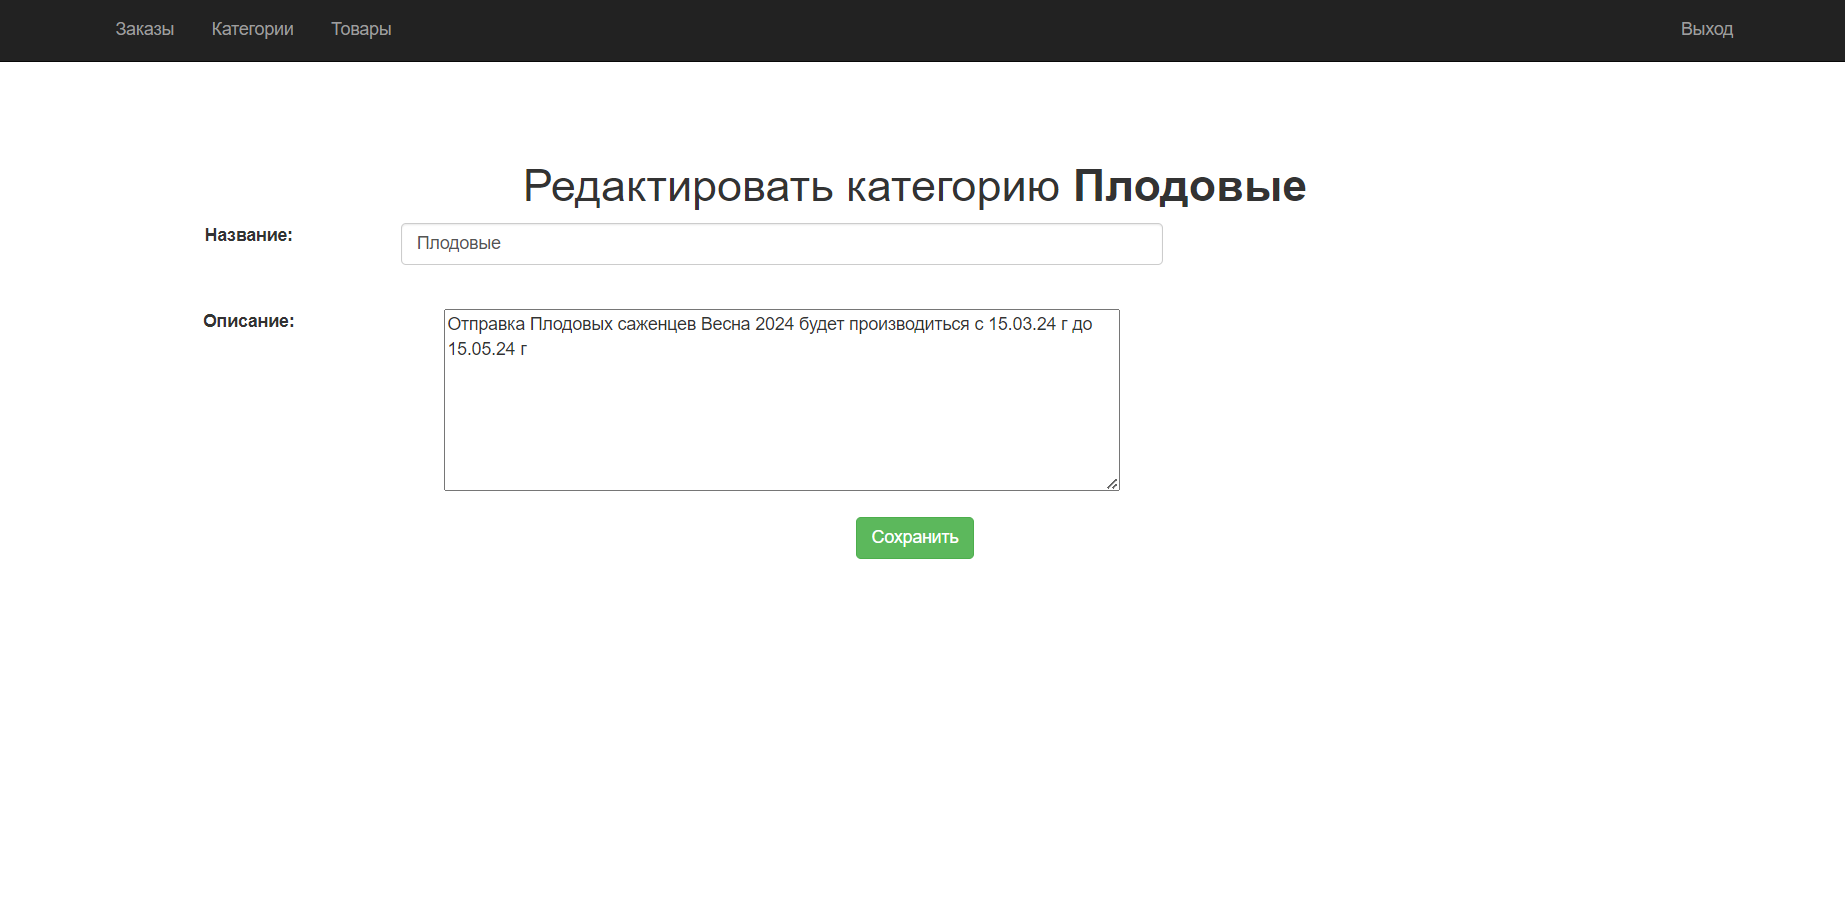
\includegraphics[width=1\linewidth]{categoryEdit}
	\caption{Страница редактирования категории в панели администратора}
	\label{categoryEdit:image}
\end{figure}
%\vspace{-\figureaboveskip} % двойной отступ не нужен (можно использовать, если раздел заканчивается картинкой)

На рисунке \ref{categoryCreate:image} показана страница создания категории в панели администратора.

\begin{figure}[H]
	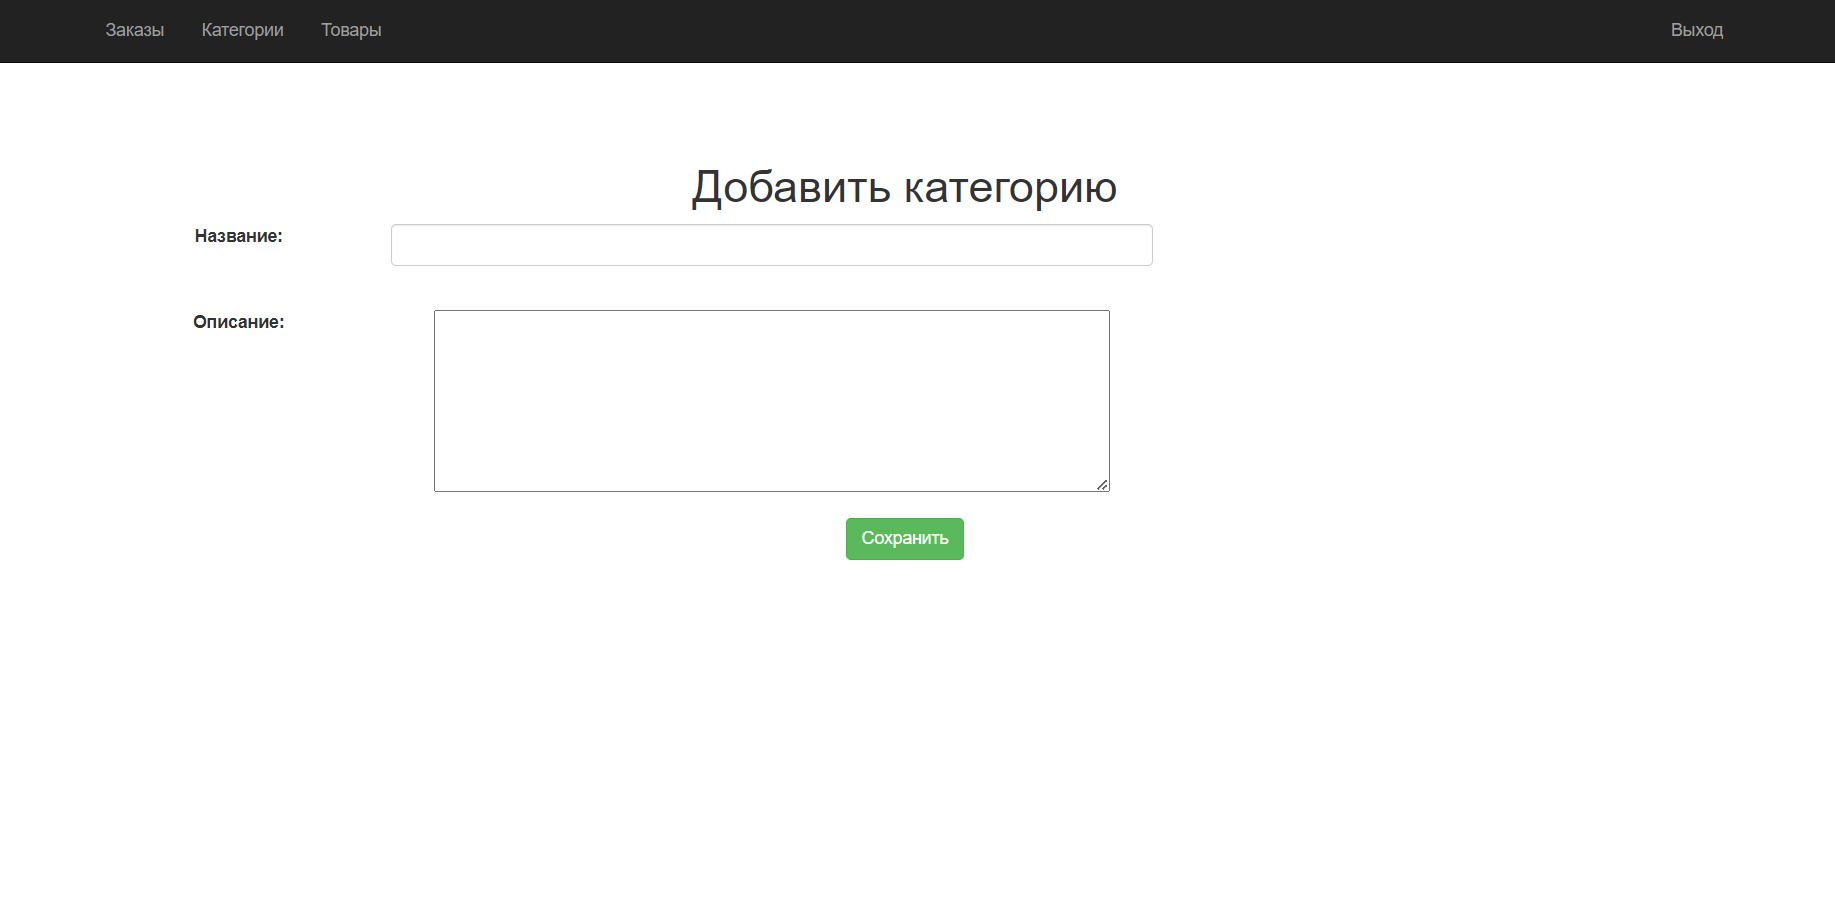
\includegraphics[width=1\linewidth]{categoryCreate}
	\caption{Страница создания категории в панели администратора}
	\label{categoryCreate:image}
\end{figure}
%\vspace{-\figureaboveskip} % двойной отступ не нужен (можно использовать, если раздел заканчивается картинкой)


На рисунке \ref{productsAdmin:image} показана страница товаров в панели администратора.

\begin{figure}[H]
	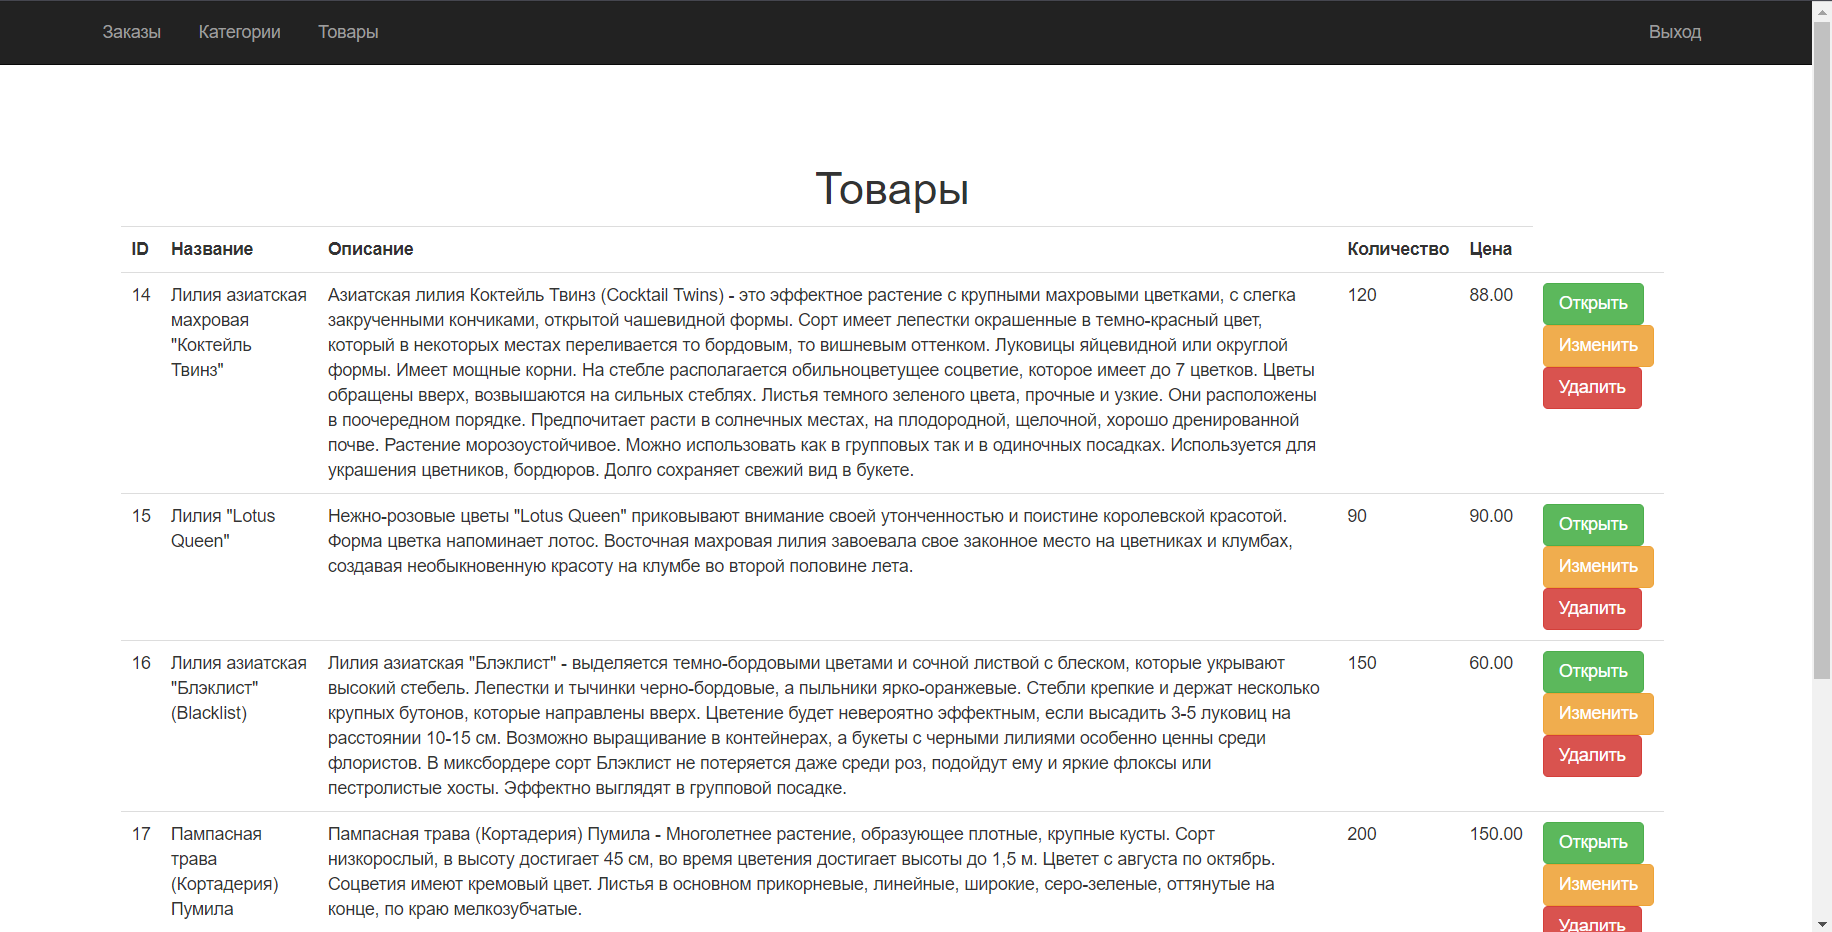
\includegraphics[width=1\linewidth]{productsAdmin}
	\caption{Страница товаров в панели администратора}
	\label{productsAdmin:image}
\end{figure}
%\vspace{-\figureaboveskip} % двойной отступ не нужен (можно использовать, если раздел заканчивается картинкой)

На рисунке \ref{productAdmin:image} показана страница одного из товаров в панели администратора.

\begin{figure}[H]
	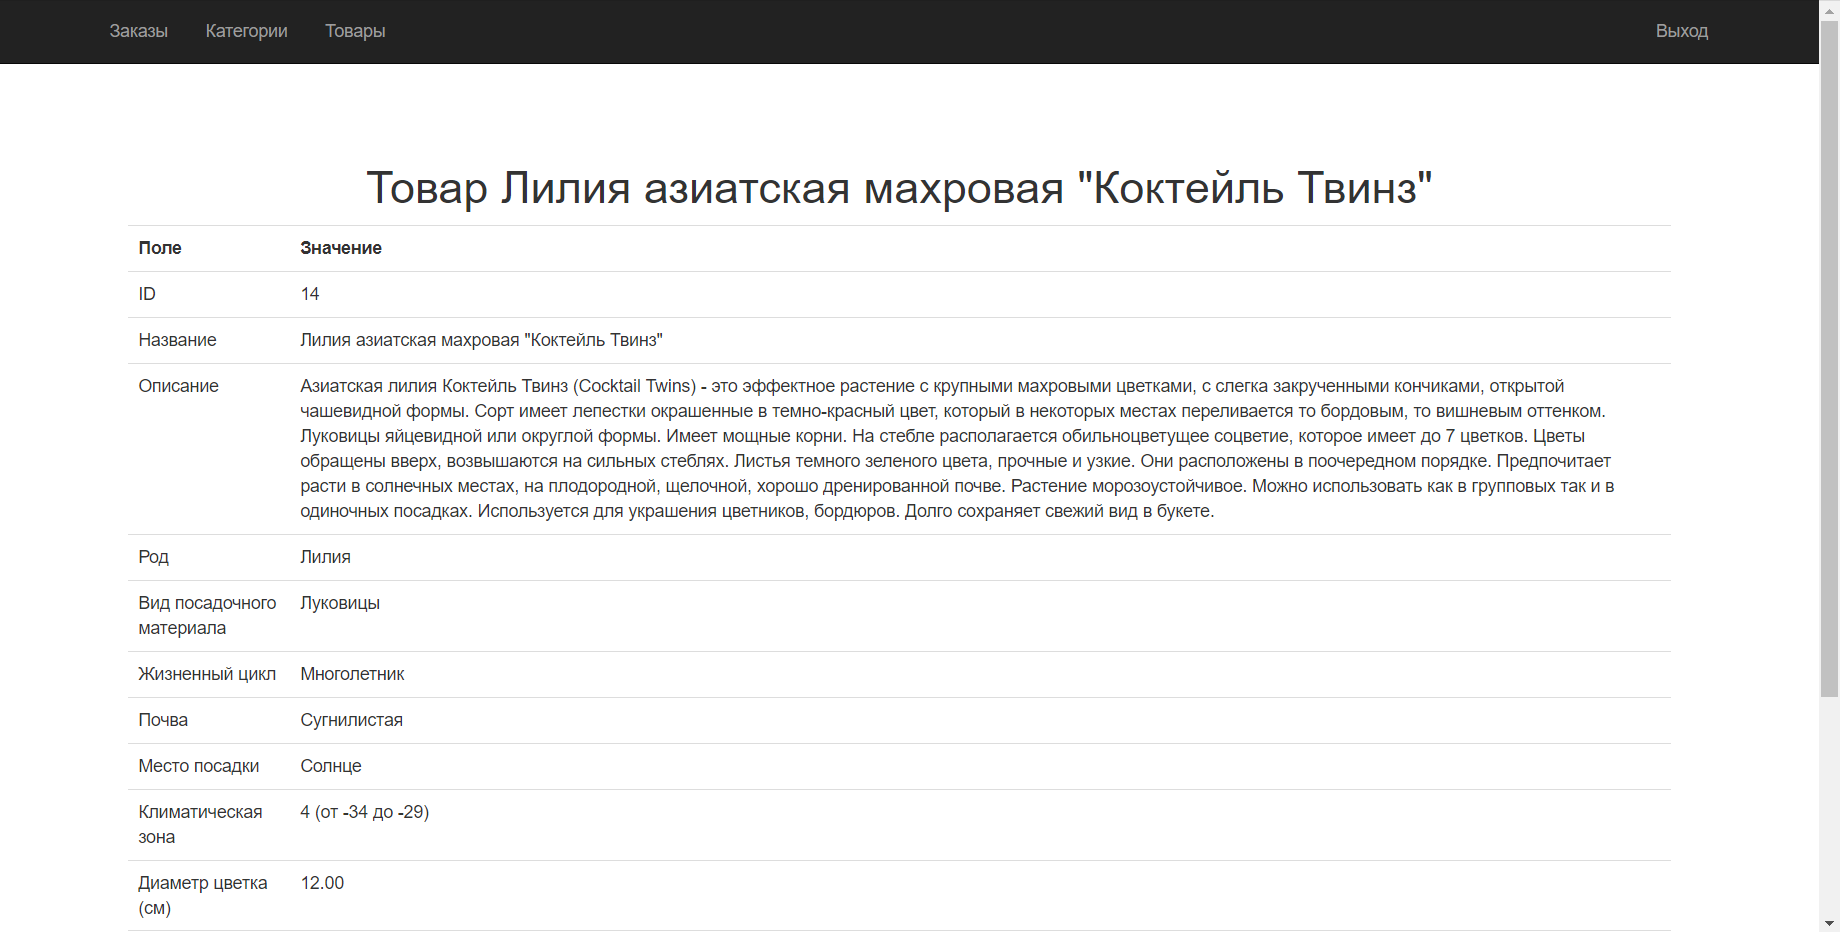
\includegraphics[width=1\linewidth]{productAdmin}
	\caption{Страница товара в панели администратора}
	\label{productAdmin:image}
\end{figure}
%\vspace{-\figureaboveskip} % двойной отступ не нужен (можно использовать, если раздел заканчивается картинкой)

На рисунке \ref{productEdit:image} показана страница редактирования товара в панели администратора.

\begin{figure}[H]
	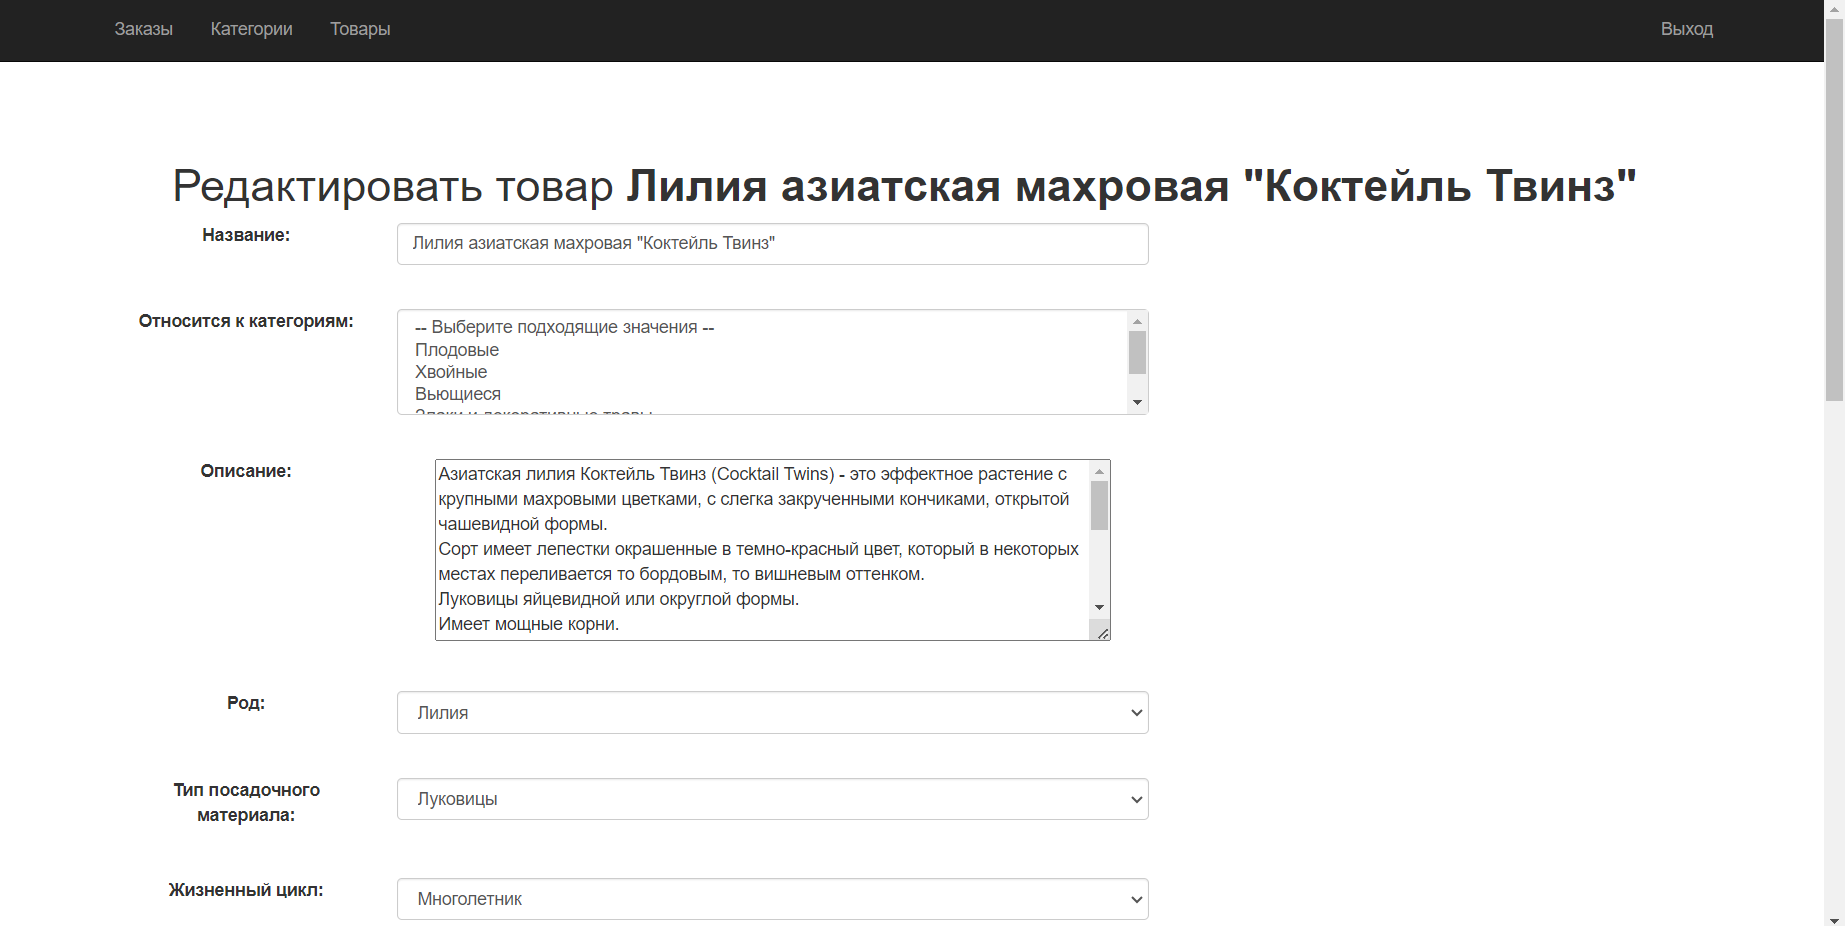
\includegraphics[width=1\linewidth]{productEdit}
	\caption{Страница редактирования товара в панели администратора}
	\label{productEdit:image}
\end{figure}
%\vspace{-\figureaboveskip} % двойной отступ не нужен (можно использовать, если раздел заканчивается картинкой)

На рисунке \ref{productCreate:image} показана страница создания товара в панели администратора.

\begin{figure}[H]
	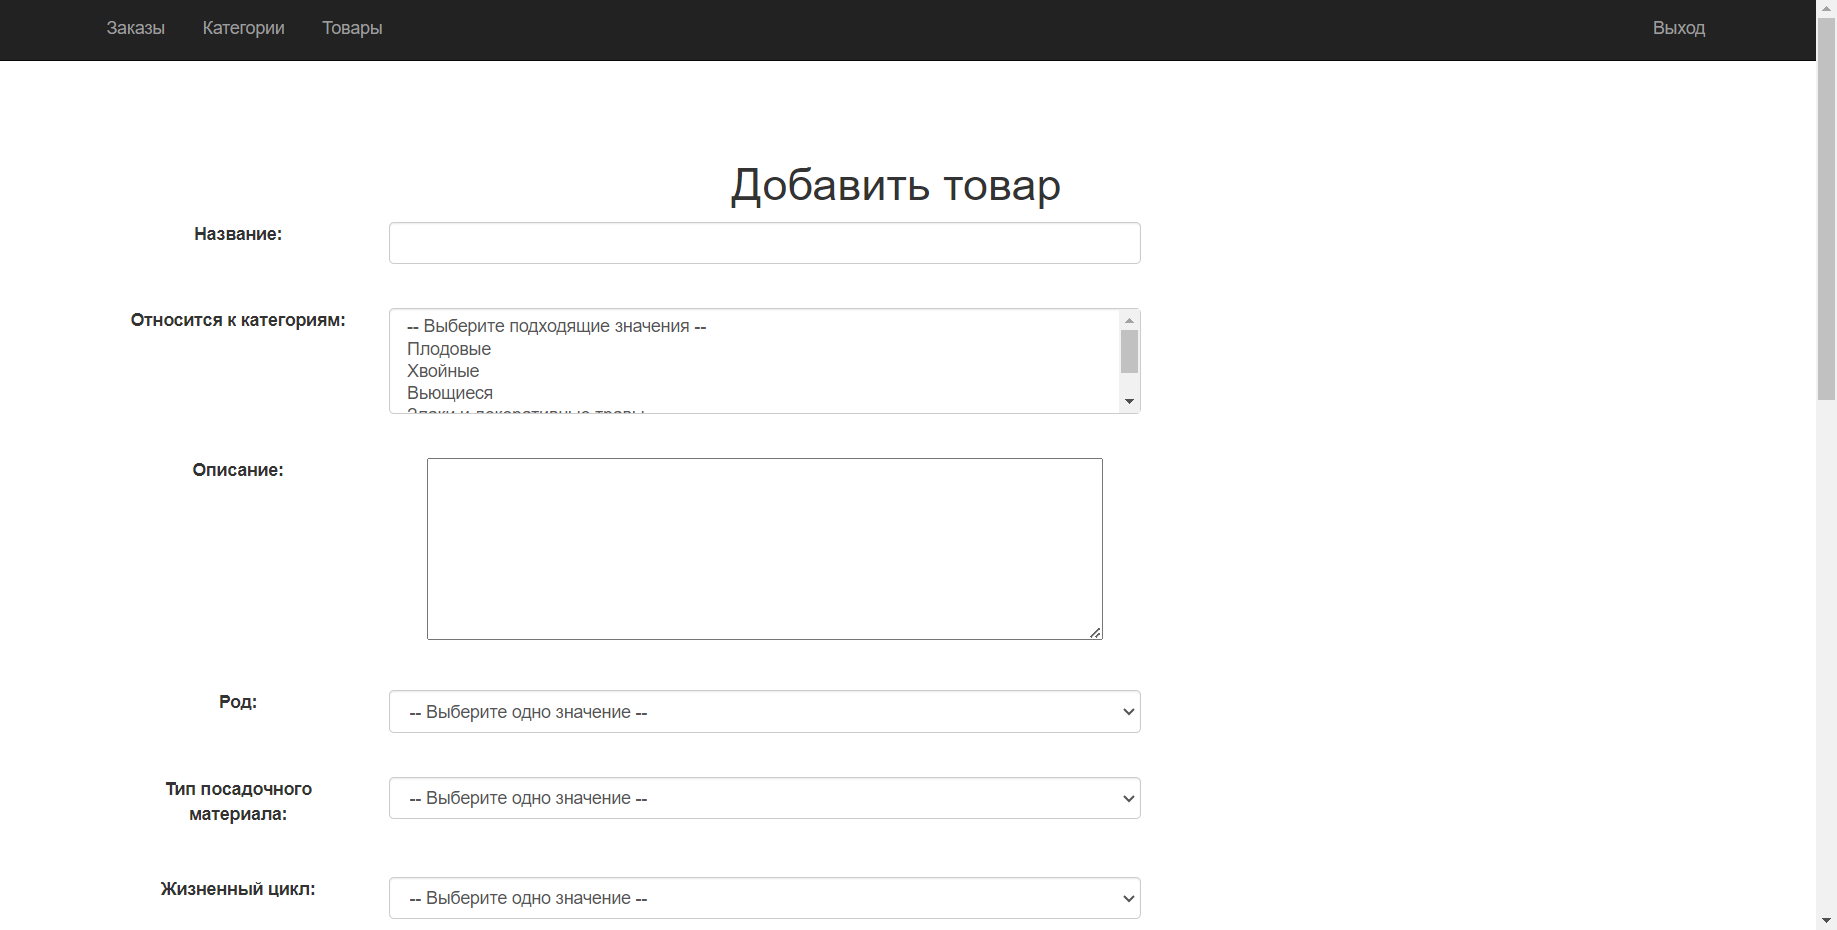
\includegraphics[width=1\linewidth]{productCreate}
	\caption{Страница создания товара в панели администратора}
	\label{productCreate:image}
\end{figure}
%\vspace{-\figureaboveskip} % двойной отступ не нужен (можно использовать, если раздел заканчивается картинкой)



   \section*{ЗАКЛЮЧЕНИЕ}
\addcontentsline{toc}{section}{ЗАКЛЮЧЕНИЕ}

В процессе выполнения данной работы была создана программно-информационная система для продажи декоративных растений. Были реализованы функции для администратора и покупателей.

Покупатели имеют возможность просматривать товары, используя фильтры по характеристикам и поиск по названию, и оформлять заказы. Администратор может просматривать список заказов, а также  контролировать товары и их категории.

Основные результаты работы:

\begin{enumerate}
	\item Проведен анализ предметной области. 
	\item Разработана концептуальная модель web-сайта. Определены требования к системе.
	\item Осуществлено проектирование web-сайта. Разработана архитектура серверной части. Разработан пользовательский интерфейс web-сайта.
	\item Реализован и протестирован web-сайт.
\end{enumerate}

Все требования, объявленные в техническом задании, были полностью реализованы, все задачи, поставленные в начале разработки проекта, были также решены.


}\fi
\addcontentsline{toc}{section}{СПИСОК ИСПОЛЬЗОВАННЫХ ИСТОЧНИКОВ}

\begin{thebibliography}{9}

    \bibitem{brett} Бретт, М. PHP и MySQL. Исчерпывающее руководство / М. Бретт. – Санкт-Петербург : Питер, 2016 г. – 544 с. – ISBN 978-5-496-01049-8. – Текст~: непосредственный.
    \bibitem{veru} Веру, Л. Секреты CSS. Идеальные решения ежедневных задач / Л. Веру. – Санкт-Петербург : Питер, 2016 г. – 336 с. – ISBN 978-5-496-02082-4. – Текст~: непосредственный.
    \bibitem{gizbert}	Гизберт, Д. PHP и MySQL / Д. Гизберт. – Москва~: НТ Пресс, 2013 г. – 320 с. – ISBN 978-5-477-01174-2. – Текст~: непосредственный.
	\bibitem{dakett}	Дэкетт, Д. HTML и CSS. Разработка и создание веб-сайтов / Д. Дэкетт. – Москва~: Эксмо, 2014 г. – 480 с. – ISBN 978-5-699-64193-2. – Текст~: непосредственный.
	
	
	\bibitem{groff} Грофф, Дж. Р. SQL: полное руководство / Грофф Дж. Р., Вайнберг П. Н., Оппель Э. Дж. — 3-е изд. — Санкт-Петербург~: Диалектика, 2020 г. — 960 c. - ISBN 978-5-907114-26-5. – Текст~: непосредственный.
	
	\bibitem{shvartz} Шварц, Б. MySQL. Оптимизация производительности  / Шварц Б., Зайцев П., Ткаченко В., Заводны Дж., Ленц А., Бэллинг Д. — 2-е изд. — Санкт-Петербург~: Символ-Плюс, 2010 г. — 832 c. - ISBN 978-5-93286-153-0. – Текст~: непосредственный.
	
	\bibitem{kingsberry} Кингсбери, Н. Основы озеленения сада  / Кингсбери Н. — 1-е изд. — Москва~: Кладезь-Букс, 2003 г. — 208 c. - ISBN: 5-93395-034-3. – Текст~: непосредственный.
	
	\bibitem{krivko} Кривко, Н. П. Питомниководство садовых культур  / Под редакцией Кривко Н. П. — Санкт-Петербург~: Лань, 2015 г. — 368 c. - ISBN: 978-5-8114-1761-2. – Текст~: непосредственный.
	
	\bibitem{konovalova} Коновалова, Т. Ю. Декоративные кустарники, или 1000 растений для вашего сада. Иллюстрированный справочник / Т. Ю. Коновалова, Н. А. Шевырева — Москва~: Фитон+, 2004 г. — 192 c. - ISBN: 5-93457-070-6. – Текст~: непосредственный.
	
	\bibitem{berd} Берд, Р. Цветущие деревья и кустарники: дизайн вашего сада и советы по выращиванию  / Ричард Берд — Москва~: АРТ-РОДНИК, 2003 г. — 159 с. - ISBN: 5-88896-089-6.  – Текст~: непосредственный.
	
	\bibitem{[hesayon]} Хессайон, Д. Г. Всё о декоративных растениях и кустарниках  / Хессайон Д. Г.   — 2-е изд.. — Москва~: Кладезь-Букс, 2007 г. — 127 c. - ISBN: 978-5-93395-238-1. – Текст~: непосредственный.
	
	\bibitem{ganighkina} Ганичкина, О. А. Декоративные растения вашего сада: деревья, кустарники, цветы / Ганичкина О.А. —  Москва~: Эксмо, 2008 г. —  222 с. - ISBN: 978-5-699-28077-3. – Текст~: непосредственный.
	
	\bibitem{marcovsky} Марковский, Ю. Б. Хвойные растения для декоративного сада / Ю. Б. Марковский, И. В. Успенский. — Москва~: Фитон XXI, 2016 г. — 232 с. - ISBN: 978-5-906171-91-7. – Текст~: непосредственный.
	
	\bibitem{kirichenko} Кириченко, А. В. Laravel для WEB-разработчиков. Практическое руководство по созданию профессиональных сайтов / А. В. Кириченко, Е. В. Дубовик. — Санкт-Петербург~:Наука и Техника, 2021 г. - 432 с. - ISBN: 
	978-5-94387-726-1. – Текст~: непосредственный.
	
	\bibitem{dronov} Дронов, В. А. Laravel. Быстрая разработка современных динамических Web-сайтов на PHP, MySQL, HTML и CSS / В. А. Дронов. — Санкт-Петербург~:БХВ-Петербург, 2018 г. - 755 с. - ISBN: 978-5-9775-3845-9. – Текст~: непосредственный.
\end{thebibliography}

\ifВКР{\appendix{Представление графического материала}

Графический материал, выполненный на отдельных листах,
изображен на рисунках А.1--А.\arabic{числоПлакатов}.
\setcounter{числоПлакатов}{0}

\renewcommand{\thefigure}{А.\arabic{figure}} % шаблон номера для плакатов

\begin{landscape}

\begin{плакат}
	\includegraphics[width=0.82\linewidth]{plakat1}
	\заголовок{Сведения о ВКРБ}
	\label{plakat1:image}      
\end{плакат}

\begin{плакат}
	\includegraphics[width=0.82\linewidth]{plakat2}
	\заголовок{Цель и задачи разработки}
	\label{plakat2:image}      
\end{плакат}

\begin{плакат}
	\includegraphics[width=0.82\linewidth]{plakat3}
	\заголовок{Диаграмма прецедентов. Часть 1}
	\label{plakat3:image}      
\end{плакат}

\begin{плакат}
	\includegraphics[width=0.82\linewidth]{plakat4}
	\заголовок{Диаграмма прецедентов. Часть 2}
	\label{plakat4:image}      
\end{плакат}

\begin{плакат}
	\includegraphics[width=0.82\linewidth]{plakat5}
	\заголовок{Диаграмма компонентов}
	\label{plakat5:image}      
\end{плакат}

\begin{плакат}
	\includegraphics[width=0.82\linewidth]{plakat6}
	\заголовок{Концептуальная модель предметной области}
	\label{plakat6:image}      
\end{плакат}

\begin{плакат}
	\includegraphics[width=0.82\linewidth]{plakat7}
	\заголовок{Страница просмотра товаров}
	\label{plakat7:image}      
\end{плакат}

\begin{плакат}
	\includegraphics[width=0.82\linewidth]{plakat8}
	\заголовок{Страница просмотра категорий товаров}
	\label{plakat8:image}      
\end{плакат}

\begin{плакат}
	\includegraphics[width=0.82\linewidth]{plakat9}
	\заголовок{Страница корзины}
	\label{plakat9:image}      
\end{плакат}

\begin{плакат}
	\includegraphics[width=0.82\linewidth]{plakat10}
	\заголовок{Заключение}
	\label{plakat10:image}      
\end{плакат}

\end{landscape}
}\fi
\ifПрактика{}\else{\appendix{Фрагменты исходного кода программы}

BasketController.php
\lstinputlisting[language=php, frame=none]{BasketController.tex}

HomeController.php
\lstinputlisting[language=php, frame=none]{HomeController.tex}

MainController.php
\lstinputlisting[language=php, frame=none]{MainController.tex}

CategoryController.php
\lstinputlisting[language=php, frame=none]{CategoryController.tex}

OrderController.php
\lstinputlisting[language=php, frame=none]{OrderController.tex}

PlantController.php
\lstinputlisting[language=php, frame=none]{PlantController.tex}

Представление layouts/master.blade.php
\lstinputlisting[language=php, frame=none]{master.tex}

Представление frontend/index.blade.php
\lstinputlisting[language=php, frame=none]{index.tex}

\ifВКР{
\newpage
\addcontentsline{toc}{section}{На отдельных листах (CD-RW в прикрепленном конверте)}
\begin{center}
\textbf{Место для диска}
\end{center}
}\fi
}\fi
\end{document}
